\documentclass[11pt]{article}
\usepackage[utf8]{inputenc}
\usepackage[margin=1in]{geometry}
\usepackage{graphicx} % Required for inserting images
\usepackage{amsfonts}
\usepackage{amsmath}
\usepackage{dirtytalk}
\usepackage{algorithm}
\usepackage{mathtools}
\usepackage{xcolor}
\usepackage{amssymb}
\usepackage[title]{appendix}
\usepackage[noend]{algpseudocode}
\usepackage{amsthm}
\usepackage{bigints}
\usepackage{thm-restate}
\usepackage{hyperref}
\hypersetup{
    colorlinks = true,
    linkcolor = blue,
    citecolor = blue
    }
    
\usepackage[
        noabbrev,
        capitalise,
        nameinlink,
    ]
    {cleveref}
\usepackage{appendix} 
\usepackage{makecell}
\usepackage{bigints}
\usepackage{mathtools}
\usepackage{subfigure}
\usepackage{booktabs}
\usepackage{bbding}
\usepackage{wrapfig}
\usepackage{bbm}
% \usepackage{authblk}
\usepackage{cleveref}
\usepackage{romannum}
\usepackage{siunitx}
\sisetup{
  separate-uncertainty = true,
  table-align-uncertainty = true,
  table-number-alignment = center,
  round-mode = places,
  round-precision = 2
}

\newtheorem{thm}{Theorem}[section]

% everyone else shares the same counter
\newtheorem{lemma}[thm]{Lemma}
\newtheorem{prop}[thm]{Proposition}
\newtheorem{corollary}[thm]{Corollary}
\newtheorem{asmpt}[thm]{Assumption}
\newtheorem{defn}[thm]{Definition}
\newtheorem{rmk}[thm]{Remark}
\newtheorem{claim}[thm]{Claim}

\usepackage[round]{natbib}
\bibliographystyle{unsrtnat}


\newcommand{\expnumber}[2]{{#1}\mathrm{e}{#2}}
\newcommand{\man}{\mathcal{M}}
\newcommand{\norm}[1]{\left\lVert#1\right\rVert}

\newcommand{\tls}[1]{{\color{cyan}[TLS: #1]}}
\newcommand{\nts}{{\color{red}[NTS]}}


\title{Locally Linear Generalized Single Index Regression}

\author{
\begin{tabular}{c c c}
\makecell[c]{Tristan Luca Saidi\textsuperscript{\(\dagger\)}\\
\href{mailto:tsaidi@andrew.cmu.edu}{\nolinkurl{tsaidi@andrew.cmu.edu}}}
&
\makecell[c]{Arun Kuchibhotla\textsuperscript{\(\dagger\)}\\
\href{mailto:karun3kumar@gmail.com}
{\nolinkurl{arunku@cmu.edu}}}
\end{tabular}\\[0.75em]
\textsuperscript{\(\dagger\)}Department of Statistics and Data Science, Carnegie Mellon University
}

\begin{document}
\pagenumbering{arabic}

\maketitle


\begin{abstract}
    In this work we propose and analyze a procedure for estimating a generalized single-index regression model. This generalized single-index regression framework models the conditional mean of the responses $y$ as a function of the covariates $x$ where the mapping is assumed to have the form $f \circ g$, where $g$ is $\beta$-H\"older with $\beta \geq 2$ and $f$ is a $C^2$ function. We propose a general procedure that operates under minimal assumptions about the distribution of covariates $x$, requiring only boundedness, sufficient smoothness and absolute continuity with respect to Lebesgue. Our procedure estimates the gradient vector $\hat v(x) \approx \nabla g(x)$, and then uses this to produce an estimate of the response function $f$ via projected kernel regression. We derive central limit theorems for gradient vector estimates $\hat{v}_x$ and regression estimates $\hat{f}(x)$, and we derive rates of convergence for our approach, illustrating that it indeed achieves the minimax rate pointwise when $\beta = 2$.  Finally, we instantiate this model in the situation where $g = \Pi$ is a closest point projection onto a compact and regular embedded $C^3$ curve $\gamma$, a setting recently studied in the literature. We also supplement our theoretical results with simulations to demonstrate the utility of our procedure.   
\end{abstract}

% \tableofcontents

\section{Introduction}

Single-index regression is a classical tool in semi-parametric statistics for regression analysis. The model typically stipulates that the response variable $y \in \mathbb{R}$ depends on the covariates $x \in \mathbb{R}^d$ through the compositional relationship $y = f(g(x)) + \varepsilon$ where $f: \mathbb{R} \to \mathbb R$ is the \emph{link} function, $\varepsilon$ is distributed according to some noise distribution, and $g(x) = \theta^\top x$ where $\theta \in \mathbb{R}^d$ is the \emph{index} vector. Many techniques have been developed for estimation and inference in this model under a variety of assumptions \citep{li1991sliced,dennis2000save,li2005contour,li2007directional, li1989regression}, as the model simultaneously offers flexibility and interpretability. Most of these methods rely heavily on the linear structure of $g$ for computational tractability, thereby avoiding the need to jointly optimize over $f$ and $g$. 

In this work we consider a modified version of the classical single-index regression model which ablates the linear structure of $g$ that we call the \emph{generalized single-index regression model}. In particular, the model instead assumes that $g: \mathbb{R}^d \to \mathbb{R}$ is an arbitrary $\beta$-H\"older function. Na\"ively, estimation in such a model would require a bi-level optimization procedure of the form
\begin{equation}\label{bilevel optimization}
    \hat f_n, \hat g_n \in \arg\min_{\hat f \in \mathcal{F}, \hat g \in \mathcal{G}}\frac{1}{n}\sum_{i = 1}^n\left|Y_i - \hat f(\hat g(X_i))\right|^2.
\end{equation}
In this work we instead propose and analyze a conceptually simple and computationally tractable estimation procedure for the generalized single-index model that we call \emph{Locally Linear Single-Index Regression} (LLSIR). A hallmark of this procedure is that it avoids the bi-level optimization problem in \Cref{bilevel optimization} through localization; in a neighborhood of an out-of-sample point $x_0$ the $g$ function is approximately linear, and one can therefore employ classical single-index techniques to estimate $\nabla g(x_0)$ up to scale. From there, one can project onto the curve defining the estimated velocity and perform nonparametric regresison. This concept underpins the LLSIR procedure, making it conceptually simple and easy to both implement and analyze.

In \Cref{sec: theoretical results}, we provide theoretical analyses of the LLSIR procedure. Because the procedure estimates $f$ through estimating $\nabla g$, our analysis falls into two corresponding categories. In our first body of analysis, we derive an influence function expansios for the estimation error $\widehat{\nabla g} - \nabla g$ (\Cref{thm: decomposition for beta}); this readily yields a central limit theorem (\cref{corr: central limit for v}) and a rate of convergence (\cref{thm: velocity risk}). In our second body of analysis, we carry out the same derivations for the regression estimator $\hat f$. In particular, we derive an influence function expansion of $\hat f - f$ (\Cref{thm: regression ptwise decomp}), a central limit theorem (\Cref{corr: central limit for f}) and a rate of convergence (\Cref{regression risk}) for $\hat f$. Finally, we pull from the literature on estimation of composition of H\"older-smooth functions, where we find that our rates are indeed minimax optimal when $g$ is $2$-H\"older. 

In \Cref{sec: single variable model}, we instantiate the LLSIR method in the context of a related, recently studied model from \citet{wu2024conditional} called the \emph{single-variable model}. The single-variable model assumes the same compositional structure as the generalized single index model, but it instead stipulates that $g$ is the nearest-point projection onto a time-parameterized curve $(\gamma(t))_{t} \subset \mathbb R^d$. The estimator proposed by \citet{wu2024conditional} requires that the covariates be concentrated near the curve $\gamma$; this therefore requires that the marginal law of the covariates depends on the marginal law of the responses, which is a somewhat unnatural assumption for a regression model. In \Cref{sec: single variable model}  we instead show that the LLSIR procedure can be applied directly to the single-variable model, and it requires no such assumption on the covariates. Finally, in \Cref{sec: simulations} we provide simulation experiments to demonstrate the utility of the LLSIR method.


% \medskip

% \noindent \emph{Our contributions.} This work contains contributions that broadly fall into two distinct, but related, categories. 

% \begin{enumerate}
%     \item 
% \end{enumerate}

\subsection{Related Work}


% In this work we consider the problem where we are given samples $\{(x_1, y_1), \dots, (x_n, y_n)\} \sim \nu$ from some distribution over $\mathbb{R}^d\times \mathbb{R}$ with density $p_{x,y}$ and we want to model the conditional mean of $y$ given $x$. The only assumption on the covariates the we impose is that the $x$-marginal of $p_{x,y}$ has bounded support. Furthermore, we assume that the conditional mean of the responses $y$ are related to the covariates $x$ through the following composition,
% \begin{equation}
%     y_i = f(g(x_i)) + \varepsilon_i \qquad \text{with } \qquad \mathbb{E}[\varepsilon_i \, | \, x_i] = 0, \operatorname{Var}(\varepsilon_i \,| \, x_i) = \sigma^2(x_i),\, \mathbb{E}[|\varepsilon_i|^3] < \infty \label{eq: the model}
% \end{equation}
% where $g$ is a particular map from $\mathbb{R}^d \rightarrow \mathbb{R}$. One can regard such a model as a generalization of the \textit{single-index} model from classical semi-parametric statistics \cite{gyorfi2002distribution}. In such a model the conditional mean of $y$ given $x$ is modeled by $f(b^{\top}x)$ for an arbitrary $b\in \mathbb{R}^d$. Under appropriate rescaling, $b^{\top}x$ can be interpreted as a projection onto a $1$-dimensional linear subspace of $\mathbb{R}^d$. In this work, we consider the general setting where $g$ is instead a $\beta$-H\"older smooth function, and we later explore a particular instantiation of $g$ that recovers the setting of \citep{wu2024conditional}. Recall that a $\beta$-smooth function $h$ is differentiable up to order $k \triangleq\lfloor{\beta}\rfloor$, and all derivatives of order $k$ are $\alpha \triangleq \beta - \lfloor \beta \rfloor$ H\"older
% \[\sup_{x \neq y}\frac{|\operatorname{D}^{k}h(x) - \operatorname{D}^k h(y)|}{\|x - y\|^\alpha} < \infty.\]
% Estimating index models for regression is a well-studied problem in semi-parametric statistics. Many inverse regression techniques have been proposed \cite{li1991sliced, li2005contour, li2007directional, dennis2000save}, where the index vector $b$ is estimated using information about the conditional density $p(x \, |\, y)$. \citet{li1991sliced} assume the so-called \textit{Linear Conditional Expectation} (LCE) property of the density of the covariates, which allows one to directly relate the curve $\mathbb{E}[x\,|\,y]$ to the index direction $b$. In particular, this LCE property ensures that for any $b \in \mathbb{R}^p$ and $B \in \mathbb{R}^{d\times p}$ there exists a $c \in \mathbb{R}^d$ such that the conditional expectation $\mathbb{E}[b^{\top}x \, | B^{\top}x] = (B^{\top}x)^{\top} c$. This assumption is weaker that it may seem -- any elliptically symmetric distribution satisfies it. It also guarantees that the solution $\theta^*$ to a linear regression with any convex cost is proportional to the index vector $\beta$ \cite{li1989regression}. Leveraging this result, \citet{Newey_Ruud_2005} propose a procedure to circumvent this assumption by using importance sampling, reweighting the observed data so that in the limit the reweighted observations are distributed according to a density satisfying the LCE property. 

% \subsection{Related Work}
Our work relates to several areas of the statistical and computer science literature. We review each area here.
\medskip

\emph{Single-index regression.}
The classical single-index model assumes that the regression function takes the form $m(x)=f(\theta^\top x)$ for an unknown ``index'' direction $\theta$ and an unknown univariate link $f$. A substantial literature studies estimation of $\theta$ under different assumptions on the covariate distribution. Inverse regression approaches, including sliced inverse regression, SAVE, contour regression, and directional regression, recover the index direction from moments of $X \,|\, Y$ \citep{li1991sliced,dennis2000save,li2005contour,li2007directional}. These methods are closely connected to the linear conditional expectation condition exploited by \citet{li1989regression}. Conversely, an abundance of methods consider the forward-regression approach. For example, average-derivative methods recover an index direction from derivatives of the regression function \citep{hardle1989average,powell1989semiparametric}, while profile and semiparametric least-squares methods jointly estimate the index and unknown link \citep{ichimura1993semiparametric,hardle1993optimal}. Iterative refinements of average-derivative estimation can also recover single- and multi-index structure at parametric rates under suitable conditions \citep{hristache2001direct,hristache2001structure}. Our construction is most directly related to the density-weighted least-squares estimator of \citet{Newey_Ruud_2005}, which reweights observations by the ratio of an elliptically symmetric target density to the covariate density so that the limiting regression problem behaves as though the design satisfied the LCE property. In contrast to these classical methods, however, we do not assume that our target direction $\nabla g$ is a fixed global index vector. Instead, the possibly nonlinear map $g$ yields a location-dependent direction $\nabla g(x_0)$ that generally varies throughout the covariate space.
\medskip 

\emph{Compositional function estimation.}
The literature regarding general models of the compositional form $m=f\circ g$ is quite rich. Most directly, \citet{juditsky2009nonparametric} study the estimation of a multivariate function represented as the composition of a univariate outer function and a multivariate inner function, and they characterize minimax estimation rates over smooth composition classes. More recently, \citet{Schmidt_Hieber_2020} establishes minimax rates for substantially more general hierarchical composition classes using sparse deep ReLU networks. 
Finally, our closest-point projection example in \Cref{sec: single variable model} is directly related to the nonlinear single-variable model of \citet{wu2026conditional}, who consider $m(x)=f(\Pi_\gamma x)$ with $\Pi_\gamma$ the closest-point coordinate associated with an unknown regular curve $\gamma$. Their estimator combines ideas from inverse regression and manifold learning, though their analysis restricts the covariate distribution to a neighborhood of the curve $\gamma$; under additional conditions on the link and variation normal to the curve, they obtain a one-dimensional minimax rate up to logarithmic and geometry-dependent effects. We remark that this setting is related to, but distinct from, regression under a manifold-support assumption. In this setting, local polynomial regression has been shown to adapt to intrinsic dimension when the covariates lie on or sufficiently near a lower-dimensional manifold \citep{bickel2007local}. Furthermore, locally-linear methods have also been developed for simultaneous regression and gradient estimation on an unknown manifold \citep{cheng2013local}. 
\medskip

\emph{Sufficient dimension reduction.}
Our work is also intimately related to the vast literature on sufficient dimension reduction for regression. \citet{cook2002dimension} formalize sufficient dimension reduction for the conditional mean through the study of the so-called ``central mean subspace", while \citet{xia2002adaptive} propose the minimum average variance estimation method which combines local linear approximations of the regression function with estimation of an informative linear subspace, placing substantially weaker restrictions on the covariate distribution than classical inverse-regression methods. Closely related procedures from \citet{xia2002adaptive} and \citet{xia2007constructive} likewise recover directions from local derivatives of the regression function. Kernel methods subsequently relaxed the linear-subspace formulation \citep{fukumizu2009kernel}, while \citet{lee2013nonlinear} developed a general theory of nonlinear sufficient dimension reduction in terms of sufficient and central classes of functions.

\medskip


\emph{Local regression and gradient estimation.}
The first stage of our procedure is also closely connected to the classical literature on local polynomial regression and nonparametric derivative estimation. Local polynomial estimators and their bias and variance expansions were developed by \citet{ruppert1994multivariate}, while \citet{lu1996partial} develops the asymptotic theory for multivariate partial derivative estimation. This literature is especially pertinent because $\nabla(f\circ g)(x_0)=f'(g(x_0))\nabla g(x_0)$, so local derivative estimation provides one route to recovering the index direction. Our approach instead extends the density-weighted linear least-squares (DWLLS) methodology of \citet{Newey_Ruud_2005} to nonlinear $g$. In this way, we retain the computational tractability and single-index interpretation of DWLLS while allowing the index to vary spatially.

% \emph{Generated covariates and two-stage nonparametric estimation.}
% Our regression estimator uses the first-stage direction estimate to construct a scalar projected covariate and therefore also belongs to the broad class of nonparametric procedures with generated regressors. \citet{mammen2012generated}, for example, derive general stochastic expansions and asymptotic distributions for nonparametric regression estimators whose covariates are themselves estimated in a preliminary nonparametric step. In our setting the generated covariate has a specific geometric form, obtained by projecting local displacements onto an estimated gradient direction, which allows the first-stage estimation error to be incorporated directly into the pointwise expansion for the final regression estimator.
\medskip



% Taken together, these literatures place the present method at the intersection of single-index regression, local polynomial derivative estimation, and structural adaptation for composite functions. The principal distinction is that we use density-weighted local regression to estimate a spatially varying index direction induced by a smooth nonlinear coordinate and then propagate that estimated direction through a second nonparametric regression stage. This differs both from classical single-index and sufficient-dimension-reduction methods, which typically seek a fixed global direction or subspace, and from generic multivariate nonparametric regression, which does not explicitly construct and exploit the local index direction.

\subsection{Setting and assumptions}


In this section we reiterate and elaborate on our modeling assumptions throughout this work. In particular, we consider the problem where we are given i.i.d. samples $\{(x_1, y_1), \dots, (x_n, y_n)\} \sim P_{x,y}$ from some probability measure $P_{x,y} \in \mathcal{P}(\mathbb{R}^d\times \mathbb{R})$ with density $p_{x,y}$, where our goal is to model the conditional mean of $y$ given $x$. We assume that the covariate distribution, represented as the $x$-marginal of $P_{x,y}$, has bounded support. Furthermore, we assume that the conditional mean of the responses $y$ are related to the covariates $x$ through the following composition,
\begin{equation}
    y_i = f(g(x_i)) + \varepsilon_i, \quad \text{with} \quad \varepsilon_i \sim \mathcal{E} \label{eq: the model}
\end{equation}
where $g$ is a $\beta$-H\"older smooth map from $\mathbb{R}^d \rightarrow \mathbb{R}$ and $\mathcal{E}$ is a error distribution over $\mathbb{ R}$. Recall that a $\beta$-smooth function $h$ is differentiable up to order $k \triangleq\lfloor{\beta}\rfloor$, and all derivatives of order $k$ are $\alpha \triangleq \beta - \lfloor \beta \rfloor$ H\"older, i.e.
\[\sup_{x \neq y}\frac{|\operatorname{D}^{k}h(x) - \operatorname{D}^k h(y)|}{\|x - y\|^\alpha} < \infty.\]
Moreover, we make the following assumptions on the law of the errors $\varepsilon_i$
\[\mathbb{E}[\varepsilon_i \, | \, x_i] = 0, \operatorname{Var}(\varepsilon_i \,| \, x_i) = \sigma^2(x_i),\, \mathbb{E}[|\varepsilon_i|^3] < \infty\]
which we consider to be quite standard for the regression setting.
\medskip 
% In the single-index setting, we know that the conditional expectation of $y$ given $x$ has the  compositional structure defined in \cref{eq: the model}, where $g:\mathbb{R}^d \rightarrow \mathbb{R}$ and $f: \mathbb{R}\rightarrow\mathbb{R}$. The classical single-index model takes $g(x) = b^{\top}x$ for some $b \in \mathbb{R}^d$, but in this work we take $g$ to be an arbitrary $\beta$-H\"older function from $\mathbb{R}^d$ to $\mathbb{R}$ in a neighborhood of the desired inference location $x_0$. 


\emph{The Linear Conditional Expectation (LCE) property.}
The Linear Conditional Expectation (LCE) property of the density of the covariates has played a prominent role in the study of single index models \citep{li1989regression, li1991sliced}, and it will be a key element of our approach. We reiterate that we do not assume the LCE property on the covariates; in the same manner as that of \citet{Newey_Ruud_2005}, we will merely leverage its properties via density reweighting. To recall its definition, the LCE assumption on a random variable $x \sim P$ guarantees that the conditional expectation of any linear transformation of a random variable with an LCE density conditioned on a \textit{secondary} linear transformation is linear in the second transformation. 

\begin{restatable}[Linear Conditional Expectation (LCE) property, \cite{Newey_Ruud_2005,ruud1986consistent}]{defn}{} \label{def: lce}
    A random variable $x \sim P$ is said to satisfy the Linear Conditional Expectation property if for any $b \in \mathbb{R}^{d}$ and $B \in \mathbb{R}^{d\times k}$, there exists a $c\in \mathbb{R}^k, a \in \mathbb{R}$ such that $\mathbb{E}[b^{\top}x \,| \,B^{\top}x ] = a +c^{\top}B^{\top}x.$
\end{restatable}

While the LCE assumption may seem stringent, it turns out that many distributions satisfy it. A subset of such distributions include zero-mean \textit{elliptically symmetric distributions}, a family that subsumes the Gaussian family. Contained in this subset are \textit{spherically symmetric distributions} -- probability measures that admit a density that is invariant under rotations.

\begin{restatable}[Elliptic and spherical symmetry]{defn}{}\label{def: spherical symmetry}
Let $\mu \in \mathbb{R}^d$ and let $\Lambda \in \mathbb{R}^{d\times d}$ with $\Lambda \succ 0$. If $P$ has a Lebesgue density
\begin{equation}
     \rho(x) \propto |\Lambda|^{-1/2}\rho^*\left((x-\mu)^{\top}\Lambda^{-1}(x - \mu)\right)
\end{equation}
and $\rho^*:[0, \infty) \rightarrow[0, \infty)$ does not depend on $\mu$, $\Lambda$, then the Lebesgue density of $P$ is said to be elliptically symmetric. If, furthermore, $\Lambda = \sigma^2I_d$, then the distribution of $x$ is said to be spherically symmetric. Equivalently, a random variable $x$ has a spherically symmetric distribution about its mean $\mu$ if for every orthogonal matrix $Q$, we have \[Q(x - \mu) \overset{d}{=} x - \mu\] where $\overset{d}{=}$ denotes equivalence in distribution. 
\end{restatable}


% \begin{restatable}[Spherically symmetric $\implies $ elliptically symmetric]{rmk}{}
%     Any spherically symmetric distribution is also zero mean and elliptically symmetric, and therefore satisfies the LCE property. 
% \end{restatable}

In this work we will leverage the properties of LCE densities, but we won't require the density of the covariates to satisfy it -- our only assumption on the covariate density only assume that the support of $x$ is contained in $\mathcal{B}(0, r)$ for some $r > 0$. We will instead employ importance sampling to re-weight observations as done in \citet{Newey_Ruud_2005}, which will allow us to use the following property of LCE densities when applied to the single index model.

\begin{restatable}[LCE Proportionality, \citet{li1989regression}]{thm}{} \label{thm: lce single index}
    Suppose that $P$ has a Lebesgue density that satisfies the LCE property and suppose that $y = f(b^{\top}x) + \varepsilon$ for some $b \in \mathbb{R}^d$, and $\mathbb{E}[\varepsilon \,| \, x] = 0$. Then under the assumptions of \citet[Theorem 2.1]{li1989regression}, the population-level optimization problem 
    \[\theta^*, \alpha^* = \arg\min_{\theta, \alpha}\mathbb{E}\big(y - \theta^{\top}x - \alpha\big)^2 \]
    admits an optimizer $\theta^* \propto b$. 
\end{restatable}
\noindent \textit{Proof}. We have 
\begin{align*}
    \mathbb{E}\big(y - \theta^{\top}x-\alpha\big)^2 &= \mathbb{E}\big(f(b^{\top}x) - \theta^{\top}x-\alpha  + \varepsilon\big)^2\\
    &= \mathbb{E}\Big[\big(f(b^{\top}x) - \theta^{\top}x-\alpha\big)^2\Big] + \mathbb{E}[\varepsilon^2]. \tag{$\mathbb{E}[\varepsilon \,|\,x]$ = 0}
\end{align*}
Analyzing the first term, 
\begin{align*}
    \mathbb{E}\Big[\big(f(b^{\top}x) - \theta^{\top}x-\alpha\big)^2\Big]&= \mathbb{E}\Big[ \mathbb{E}\Big[\big(f(b^{\top}x) - \theta^{\top}x-\alpha\big)^2 \, \Big | \, b^{\top}x\Big] \Big] \\
    &\geq \mathbb{E}\Big[ \Big(f(b^{\top}x) - \mathbb{E}\big[\theta^{\top}x |b^{\top}x\big]-\alpha\Big)^2 \Big] \\
    &= \mathbb{E}\Big[ \Big(f(b^{\top}x) - Cb^{\top}x-\alpha'\Big)^2 \Big]
\end{align*}
where the penultimate line uses Jensen's inequality and the last line uses the LCE property. Observe that the inequality becomes an inequality when $\theta = Cb$ and $\alpha = \alpha'$ from which the theorem follows. 

\qed{}

\Cref{thm: lce single index} tells us that the ordinary least squares estimator recovers the index vector $b$ of a single index model when the covariate density satisfies the LCE property. \citet{Newey_Ruud_2005} leverage this fact to construct an estimator of the index vector they call \emph{Density Weighted Linear Least Squares} (DWLLS) by using density reweighting to weight observations so they are asymptotically distributed according to a LCE density. In this work we combine this principle with localization to estimate the nonlinear single index model. 

\section{The estimator}

Our estimation procedure, which we call \emph{Locally Linear Single Index Regression} (LLSIR), will be constructed as follows. For an out of sample point $x_0 \in \operatorname{int}(\operatorname{supp}(P_x))$ LLSIR first estimates $\nabla g(x_0)$ by modifying and localizing the DWLLS estimator. With an estimate of $\nabla g(x_0)$, LLSIR then estimates the conditional mean $f$ by projecting nearby observations onto $\nabla g(x_0)$ and applying kernel regression. We describe our gradient estimation procedure in detail in \Cref{sec: gradient estimation}, while we describe our regression estimation procedure in \Cref{sec: regression est}. In subsequent sections, we analyze LLSIR by deriving limit theorems for $\hat f$ and $\nabla g$ as well as rates of convergence. 

\subsection{Estimating the gradient $\nabla g$} \label{sec: gradient estimation}

To localize DWLLS and estimate the gradient $\nabla g$ at some $x_0 \in \operatorname{int}(\operatorname{supp}(P_x))$, LLSIR employs the following procedure. Let $\epsilon > 0$ and consider a first-order Taylor expansion of $g$ on the $\epsilon$-ball $\mathcal{B}(x_0,\epsilon)$. \footnote{In this work we take $\mathcal{B}(\cdot, \cdot )$ to be the \textit{closed} ball.} Assuming some local regularity on $f$, one can informally write
\begin{equation} \label{eq: surrogate decomposition curve}
    f(g(x)) \approx f(g(x_0) + \nabla g(x_0)(x - x_0)) \qquad \text{for all }x \in \mathcal{B}(x_0, \epsilon).
\end{equation}
This creates a local and, critically, \textit{linear} \say{surrogate} single-index problem with an index vector proportional to $\nabla g(x_0)$. This, in turn, allows us to apply an estimator similar in flavor to that of \citet{Newey_Ruud_2005},
\begin{align} 
\widehat{\beta}_{x_0,\epsilon}, \widehat{\alpha}_{x_0, \epsilon} &= \arg\min_{\beta \in \mathbb{R}^d,\, \alpha \in \mathbb{R}} \sum_{i = 1}^{n}\mathbbm{1}_{\{x_i \in \mathcal{B}(x_0, \epsilon)\}}\frac{p^*(x_i - x_0)}{\hat{p}(x_i)}\left(y_i - (x_i - x_0)^{\top}\beta - \alpha\right)^2 
\end{align}
where $\hat{p}$ is some consistent estimate of the density of $P_x$ and $p^*$ is some spherically symmetric reference density, as defined in \Cref{def: spherical symmetry}. The density ratio re-weights each observation's contribution so that $x$ has a limiting spherically symmetric (and thus LCE) density. This means the solution to the population ordinary least squares optimization recovers the index vector of the linear surrogate problem, $\nabla g(x_0)$. We prove this formally in \Cref{lemma: surrogate problem}. By a slight abuse of notation, we'll redefine each $x_i$ to have $x_0$ subtracted off and we'll let $X_i = \begin{bmatrix}
    1 & x_i/\epsilon
\end{bmatrix}^{\top}$ to handle the intercept -- note that rescaling simplifies following calculations and provides numerical stability. The optimization problem above then becomes 
\begin{align} 
\widehat{\beta}_{x_0,\epsilon} &= \arg\min_{\beta \in \mathbb{R}^{d+1}} \sum_{i = 1}^{n}\hat{w}_i\left(y_i - X_i^{\top}\beta\right)^2 \qquad \text{with }\qquad \hat{w}_i = \mathbbm{1}_{\{x_i \in \mathcal{B}(0, \epsilon)\}}\frac{p^*(x_i)}{\hat{p}_{x}(x_i)}
\end{align}
where $\hat{p}_{x}$ is now a consistent estimate of the density of $x - \,x_0$. Through a straightforward calculation one would find that
\begin{align}
    \widehat{\beta}_{x_0,\epsilon} &= \left(\sum_{i = 1}^n\hat{w}_iX_iX_i^{\top}\right)^{-1}\left(\sum_{i = 1}^n\hat{w}_iX_iy_i\right). \label{eq: sample est closed form}
\end{align}
A similar set of calculations leads to the population quantity. We will again abuse notation and assume that $x$ has had $x_0$ subtracted off. The population optimization problem then looks like
\begin{align}
\beta^*_{x_0, \epsilon} &= \arg\min_{\beta \in \mathbb{R}^{d+1}} \mathbb{E}_{p_{x}} \Big[w\Big(f(g(x + x_0)) - X^{\top}\beta \Big)^2\Big] \qquad \text{with }\qquad w = \mathbbm{1}_{\{x \in \mathcal{B}(0, \epsilon)\}}\frac{p^*(x)}{p_{x}(x)}\label{eq: population estimator}
\end{align}
where $p_{x}$ is the density of the random variable $x - x_0$. Solving for $\beta^*_{x_0, \epsilon}$ yields
\begin{align}
    \beta^*_{x_0, \epsilon} = \mathbb{E}_{p^*}\left[\mathbbm{1}_{\{x \in \mathcal{B}(0,\epsilon)\}}XX^{\top}\right]^{-1}\mathbb{E}_{p^*}\left[\mathbbm{1}_{\{x \in \mathcal{B}(0,\epsilon)\}}Xf(g(x+x_0))\right]. \label{eq: population estimator closed form}
\end{align}
We will show that the last $d$ entries of $\widehat{\beta}_{x_0,\epsilon}$ are a consistent estimate of $\nabla g(x_0)$ up to scale, and admit a Gaussian limit centered at the population value. To formalize this, let $V = \begin{bmatrix} 0 & I_d\end{bmatrix}$ and define the population and sample approximation of $\nabla g(x_0)$ as
\begin{equation}
    v^*_{x_0, \epsilon} = V\beta^*_{x_0, \epsilon} \qquad \text{and }\qquad \hat{v}_{x_0, \epsilon} = V\hat{\beta}_{x_0, \epsilon}. \label{eq: velocity estimator}
\end{equation}


\emph{Density Estimation}. Note that the estimator in \cref{eq: sample est closed form} requires an estimate of the density ratio $p^*(x_i)/p_{x}(x_i)$. In the subsequent paragraphs we will discuss kernel density estimation, and we will impose some sufficient assumptions on the form of kernel that ensures a sufficient rate of convergence for the density estimator $\hat{p}_{x}\to p_{x}$. We begin with some standard definitions.
\begin{restatable}[Kernel order]{defn}{}
    A kernel $K$ is of order $s \in \mathbb N$ if 
    \[\int_{\mathbb{R}^d}\|u\|_2^jK(u)du < \infty, \quad \text{and}\quad \int_{\mathbb{R}^d}u_1^{j_1}\dots u_d^{j_d}K(u) du = 0, \text{where } \sum_kj_k = j\]
    for all $1 \leq j \leq s$ and 
    $\int_{\mathbb{R}^d}K(u)du = 1.$
\end{restatable}
A sufficiently high order kernel ensures that the bias $h^s$ of the density estimate has a dependence on the H\"older smoothness $s$ of the population density instead of the ambient dimension $d$ \citep[Proposition 1.2]{tsybakov2009introduction}. Let $K:\mathbb{R}^d \rightarrow \mathbb{R}$ denote a $s^{\text{th}}$ order kernel and define the kernel density estimate of $p_{x}$ as
\begin{equation}
    \hat{p}_{x}(x) = \frac{1}{nh^d}\sum_{i = 1}^nK\left(\frac{x -x_i}{h}\right). \label{eq: kde}
\end{equation}
We will impose the following further assumptions on the kernel in order to guarantee \emph{uniform} convergence in probability of $\hat{p}_{x}$ to the true density $p_{x}$.


\begin{restatable}[Further kernel assumptions, \cite{hansen2008uniform}]{asmpt}{} \label{further kernel assumptions}
    Suppose that the kernel $K$ is symmetric and satisfies $\|K\|_{\infty} < \infty$ and 
    \[\int_{\mathbb{R}^d}|K(u)|\,du_1\dots du_d < \infty.\]
    Moreover, suppose that the kernel $K$ satisfies $\int_{\mathbb{R}^d}\|u\|_2^s|K(u)|du  < \infty$ where $s$ is the order of the kernel, assume that the kernel is differentiable, assume that $\left|\frac{\partial}{\partial u}K(u)\right| \leq \Lambda_1$ for some $\Lambda_1 > 0$ and for some $\nu > 1$, and finally assume that $\left|\frac{\partial}{\partial u}K(u)\right| \leq \Lambda_1\|u\|_2^{-\nu}$ for $\|u\|_2$ sufficiently large.
\end{restatable}
Under these assumptions, we can invoke a uniform convergence in probability result from \citet{hansen2008uniform}. This will be used heavily in our influence function expansion in the proof of \Cref{thm: decomposition for beta}.
\begin{restatable}[Uniform convergence over a bounded set, \citet{hansen2008uniform}]{lemma}{} \label{lemma: uniform convergence of kde}
    Suppose that $\|p_{x}\|_{\infty}< \infty$ and the $s^{\text{th}}$ derivative of $p_{x}$ is uniformly continuous, where $s$ is the order of the kernel $K$. Moreover, suppose that \Cref{further kernel assumptions} holds. Then for any sequence $\epsilon_n  = O(1)$ we have
    \[\sup_{x \in \mathcal{B}(0, \epsilon_n)}\left|\hat{p}_{x}(x) - p_{x}(x)\right| = O_p\left(\sqrt{\frac{\log n}{nh^d}} +h^s \right)\]
    when $h \to 0$ and $nh^d/\log n \to \infty$.
\end{restatable}

\subsection{Estimating the regression function} \label{sec: regression est}

In this section we describe the LLSIR procedure to estimate the conditional mean of of the response given an out of sample point $x_0$. In particular, we will project neighboring covariates onto our estimate of the gradient of $g$ at $x_0$, denoted $\hat v_{x_0, \epsilon} \approx \nabla g(x_0)$. These projections will represent an estimate of $g(x) - g(x_0)$ up to scale, from which we can use $1$-dimensional nonparametric regression to estimate the responses.

\begin{algorithm}[h]
    \begin{algorithmic}[1]
        \caption{Locally Linear Single Index Regression (LLSIR)}
        \label{alg: LLSIR}
        \Require New sample $x_0$, samples $\{(x_i, y_i)\}_{i=1}^n \subseteq \mathbb{R}^d \times \mathbb{R}$, a density estimation kernel $K$ and bandwidth $h$, localization parameter $\epsilon$, LCE density $p^*$, nonparametric regression kernel $K_r$ and bandwidth $h_r$.\\
        Compute localized density ratios \[\hat{w}_i = \mathbbm{1}_{\{x_i - x_0 \in \mathcal{B}(0, \epsilon)\}}\frac{p^*(x_i - x_0)}{\hat p_{x}(x_i) } \qquad \text{where} \qquad \hat p_{x}(x) = \frac{1}{nh^d}\sum_{i = 1}^nK\left(\frac{x -x_i}{h}\right)\]for all $i \in \{1, \dots, n\}$. \\
        Center and augment data, $X_i = \begin{bmatrix}
            1 & \frac{x_i - x_0}{\epsilon}
        \end{bmatrix}^{\top}$ for all $i \in \{1, \dots , n\}.$ \\
        Compute velocity estimate as 
        \[ \hat{v}_{x_0, \epsilon} = V\left(\sum_{i = 1}^n\hat{w}_iX_iX_i^{\top}\right)^{-1}\left(\sum_{i = 1}^n\hat{w}_iX_iy_i\right) \qquad \text{with} \qquad V = \begin{bmatrix}
            0 & I_d
        \end{bmatrix}.\] \\
        Normalize velocity estimate, $\hat v_{x_0, \epsilon}' = \hat v_{x_0, \epsilon} /\|\hat v_{x_0, \epsilon}\|_2$.\\
        Obtain neighborhood projection as $\hat{z}_i = \langle x_i - x_0, \hat{v}'_{x, \epsilon} \rangle$. \\
        Estimate response as 
        \begin{equation} \label{eq: kernel regressor}
            \hat{f}(x_0) = \frac{\sum_{i=1}^n \mathbbm{1}_{\{x_i\in \mathcal{B}(x_0, \epsilon)\}}y_iK_r(\frac{\hat{z}_i}{h_r})}{\sum_{i=1}^n \mathbbm{1}_{\{x_i\in \mathcal{B}(x_0, \epsilon)\}}K_r(\frac{\hat{z}_i}{h_r})}.
        \end{equation}
        \Return $\hat{f}(x_0)$
    \end{algorithmic}
\end{algorithm}

Our entire procedure for estimating the generalized single index model, which we call Locally Linear Single Index Regression (LLSIR), is described in \Cref{alg: LLSIR}. We note that we impose an additional assumption on the nonparametric regression kernel $K_r:\mathbb{R} \rightarrow \mathbb{R}$, described in \cref{assumption: kernel nondegeneracy}. This assumption is standard for localization kernels, and it allows us to bound quantities in a straightforward manner.

\begin{restatable}[Local non-degeneracy of $K_r$]{asmpt}{} \label{assumption: kernel nondegeneracy}
    We assume that the nonparametric regression kernel $K_r$ satisfies \cref{further kernel assumptions} and has $K'_r(0) = 0$, with bounded first, second and third derivatives. We also require that the kernel $K_r$ is Lipschitz and that there exist constants $\delta > 0$ and $k_r > 0$ such that 
    \[|u| \leq \delta \implies K_r(u) \geq k_r.\]
\end{restatable}


Clear from \Cref{alg: LLSIR} is the fact that the method is algorithmically simple. The velocity estimation stage to produce $\hat v_{x_0, \epsilon}$ has a simple matrix-algebraic closed form, while the conditional mean estimation is simply univariate kernel regression. This is in stark contrast to the na\"ive bilevel optimization problem in \Cref{bilevel optimization} for estimating the generalized single index model.

\subsection{Identifiability}

Before presenting our theoretical analyses of the LLSIR procedure, we will briefly remark on the nuances of identifiability. In particular, we cannot expect that, in general, $f$ and $g$ can be uniquely identified. Indeed, taking $\tilde f(z) = f(z + c)$ and $\tilde g(x) = g(x) - c$ gives $(\tilde f \circ \tilde g)(x) = (f \circ g)(x) = m(x)$ yielding an immediate counterexample. In fact, this can be generalized to any invertible $h: \mathbb{R}\to \mathbb{R}$, taking $\tilde f = f \circ h^{-1},$ and $\tilde g = h \circ g$ gives $m(x) = (f\circ g)(x) = (\tilde f \circ \tilde g)(x)$. Despite this, one can show that $\nabla g$ can be identified up to scale pointwise almost surely under reasonable assumptions about $f, g$. 

\begin{prop}[Identification of $\nabla g(x_0)$ up to scale]\label{identification}
    Suppose $x_0 \sim P_x$ and define the critical sets of $f, g$ as
    \[\mathcal{C}_f = \{t : f'(t) = 0\}, \quad \mathcal{C}_g = \{x : \nabla g(x) =0\}.\]
    Then if $f$ and $g$ satisfy $\mathcal{L}_1(\mathcal{C}_f) = \mathcal{L}_d(\mathcal{C}_g) = 0$ where $\mathcal{L}_d$ is the $d$-dimensional Lebesgue measure on $\mathbb{R}^d$, then $\operatorname{span}\{\nabla g(x_0)\}$ is identifiable $P_x$-almost-surely.
\end{prop}
\begin{proof}
    The proof of the statement above is quite simple. We seek to show that if $f \circ g \equiv \tilde f \circ \tilde g$, then under the stated assumptions $\operatorname{span}\{\nabla g(x_0)\} = \operatorname{span}\{\nabla \tilde g(x_0)\}$ $P_x$-a.s. To see this, note that since $P_x \ll \mathcal{L}_d$, we have $P_x(\mathcal{C}_g) = 0.$ Moreover, the $\beta \geq 2$ H\"older regularity of $g$ that we have assumed guarantees that $g_{\#}P_x \ll \mathcal{L}_1$, and therefore $P_x(g^{-1}(\mathcal{C}_g)) = 0$ because $\mathcal{L}_1(\mathcal{C}_f) = 0.$ Thus, we have shown that for $x \sim P_x$, $f'(g(x_0)) \neq 0 $ and $\nabla g(x_0) \neq 0$ almost surely.

    Now suppose that $\tilde f \circ \tilde g = f \circ g$. Differentiating both sides at an $x \in \mathbb{R}^d$ such that neither $f(g(x))$ nor $g(x)$ are critical gives
    \begin{align*}
        \tilde f'(\tilde g(x)) \cdot \nabla \tilde g(x) = f'(g(x)) \cdot \nabla g(x).
    \end{align*}
    Since neither sides are $0$ almost surely, then $\operatorname{span}\{\nabla \tilde g(x_0)\} = \operatorname{span}\{\nabla g(x_0)\} \neq \{0\}$, and the conclusion follows. 
\end{proof}

We remark that the conditions on the critical sets of $f$ and $g$ in \Cref{identification} are fairly mild. For instance, any functions with a countable number of stationary points would be satisfactory. The implications of this result guided the theoretical results to follow, as we cannot possibly hope to recover $g$ directly. Instead, we prove convergence results of the form $\hat v_{x_0, \epsilon} \to c_*\nabla g(x_0)$ where $c_* \in \mathbb{R}$ is an unknown scalar.

\section{Convergence} \label{sec: theoretical results}

In this section we present theoretical results regarding the LLSIR procedure. To provide an overview, we prove a central limit theorem for both the gradient $\hat{v}_{x_0, \epsilon}$ (\Cref{corr: central limit for v}) and the response estimate (\Cref{corr: central limit for f}); the limiting normal for the former is indeed centered at its population counterpart, while the limiting normal for the latter has an asymptotic bias that can be eliminated with an undersmoothing condition. As an intermediate result, we derive influence function expansions for the gradient $\hat{v}_{x_0, \epsilon}$ and the response $\hat f$ in \Cref{thm: decomposition for beta} and \Cref{thm: regression ptwise decomp} respectively. Before detailing these results, we will outline our main assumptions on the model, the reference density $p^*$, and the covariate law $p_x \, dx = P_x$.

\begin{restatable}{asmpt}{} \label{assumption: lce and covariate density}
    We require that $p^*(x)$ be a zero-mean spherically symmetric density with isotropic covariance. Moreover, we require the following:
    \begin{enumerate}
        \item (LCE density): the density $p^*(x)$ satisfies $\mathbb{E}_{p^*}[XX^{\top}] \succ 0$, is continuous at $0$, and satisfies $p^*(0)>0$.
        \item (Covariate support): We assume that the support of the covariates is bounded, i.e.  for some $r > 0$ \[\overline{\{x : p_{x}(x) \neq 0\}} \subseteq \mathcal{B}(0, r).\]
        \item (Covariate density): there exists a non-negative integer $s \geq 1$ such that the $s^{\text{th}}$ derivative of the density $p_{x}(x)$ is uniformly continuous.
        \item (Noise regularity): at the out of sample point $x_0$, $\sigma^2(x)$ is continuous at $x_0$, $\sigma^2(x_0)>0$, and there exists $\delta>0$ such that
        \[
            \sup_{x\in\mathcal{B}(x_0,\delta)}
            \mathbb{E}[|\varepsilon|^3\mid x] < \infty.
        \]
    \end{enumerate}
\end{restatable}


\subsection{Gradient estimate} \label{sec: velocity results presentation}

To analyze the convergence of $\hat v_{x_0, \epsilon}$ to its (scaled) population counterpart $c_*\nabla g(x_0)$, we will decompose
\[\hat v_{x_0, \epsilon} - c_* \nabla g(x_0) = \underbrace{\hat v_{x_0, \epsilon} - v^*_{x_0, \epsilon}}_{\text{statistical error}} + \underbrace{v^*_{x_0, \epsilon} - c_* \nabla g(x_0)}_{\text{localization bias}} \]
In particular, we will first show that the population quantity $v^*_{x_0, \epsilon}$ converges to the desired quantity $\nabla g(x_0)$ up to scale at an $\epsilon^2$ rate. This is formalized in \Cref{thm: population prop}.

\begin{restatable}[Bias shrinkage with localization]{thm}{}\label{thm: population prop}
    For some scalar $c_* \in \mathbb{R}$, $P_x$-almost every $x_0 \in \mathcal{B}(0, r)$ and $\epsilon$ sufficiently small we have 
    \[\|v^*_{x_0, \epsilon} - c_*\nabla g(x_0)\|_2 \lesssim \epsilon^2\]
    with $v^*_{x_0, \epsilon}$ defined in \cref{eq: velocity estimator}. Moreover, we have the explicit expression
    \[c_* = \epsilon f'(g(x_0))+ o(\epsilon^2).\]
\end{restatable}

The proof of \Cref{thm: population prop} is provided in \Cref{sec: proof of population vel prop}. This result establishes that the rate with which the bias induced by localization (or rather, lack thereof) shrinks as a function of the localization parameter $\epsilon$. Our next result instead considers the deviation between the population quantity $v^*_{x_0, \epsilon}$ and the sample estimator $\hat v_{x_0, \epsilon}$ -- in particular, we provide an influence function expansion of the difference, which will later allow us to establish a central limit theorem and rates of convergence. This influence function expansion is described in \Cref{thm: decomposition for beta}

\begin{restatable}[Velocity error expansion]{lemma}{} \label{thm: decomposition for beta}
    Suppose that \cref{further kernel assumptions} and \cref{assumption: lce and covariate density} are satisfied, and suppose that the density kernel bandwidth satisfies $h \asymp n^{-1/(2s+d)}$, $\epsilon \rightarrow 0, n\epsilon^d \rightarrow \infty$ and $\sqrt{n\epsilon^d}n^{-s/(2s+d)} \to 0$. Finally, suppose that $p_{x}$ is bounded away from zero on $\mathcal{B}(0, \epsilon)$ (where $p_{x}$ is the density of $x - x_0$). Then it holds that
    \[\hat{v}_{x_0, \epsilon} - v^*_{x_0, \epsilon} = \frac{1}{n}VQ^{-1}\sum_{i = 1}^nw_iX_i(u_i - \mathbb{E}[u_i\,|\,X_i]) +o_p\left(\frac{1}{\sqrt{n\epsilon^{d}}}\right)\]
    where $u = y - X^{\top}\beta_{x_0, \epsilon}^*$ and $Q = \mathbb{E}[wXX^{\top}]$.
\end{restatable}
The proof of \Cref{thm: decomposition for beta} is provided in \Cref{sec: proof of velocity decomp}. Having established this influence function expansion, we will now use it to characterize the limiting distribution of $\hat{v}_{x_0, \epsilon} - v^*_{x_0, \epsilon}.$ To do this, we will appeal to the multivariate Lyapunov central limit theorem, described in \Cref{thm: lyapunov clt}.

\begin{restatable}[Central limit for $\hat{v}_{x_0, \epsilon}$]{thm}{} \label{corr: central limit for v}
    Suppose \cref{further kernel assumptions} and \cref{assumption: lce and covariate density} hold, suppose that the assumptions of \Cref{thm: decomposition for beta} are satisfied, and suppose that $\epsilon/h \to0 $. Further let $V = \begin{bmatrix}
        0 & I_d
    \end{bmatrix}$, $\Lambda = \operatorname{Cov}(wX(u - \mathbb{E}[u\,|\,X]))$ and $u = y - X^{\top}\beta_{x_0, \epsilon}^*$. Then we have asymptotic normality of the velocity vector estimate $\hat{v}_{x_0, \epsilon}$,
    \[\sqrt{n\epsilon^{d}}(\hat{v}_{x_0, \epsilon} - v^*_{x_0, \epsilon}) \overset{d}{\rightarrow}N(0, \Sigma(x_0))\]
    where 
    \[\Sigma(x_0) = \frac{(d+2)\sigma^2(x_0)}{p_x(x_0)\mathcal{L}(\mathcal{B}(0,1))} I_d.\]
\end{restatable}
We provide the proof of \Cref{corr: central limit for v} in \Cref{sec: proof of central limit for v}. This result characterizes the limiting distribution of the gradient estimate $\hat v_{x_0, \epsilon}$ centered at its biased population counterpart $v^*_{x_0, \epsilon}$. The proof involves verifying that the random variables in the influence function expansion derived in \Cref{thm: decomposition for beta} satisfy the Lyapunov condition of \Cref{thm: lyapunov clt}. Combining the influence function expansion and the bias rate immediately yields a stochastic convergence rate for the estimator for a fixed out of sample point $x_0$. 

\begin{restatable}[Risk of $\hat{v}_{x_0, \epsilon}$]{corollary}{} \label{thm: velocity risk}
    If we choose $\epsilon \asymp n^{-1/(d+4)}$ then we have
    \[\left\|\hat{v}_{x_0, \epsilon} - c_*\nabla g(x_0)\right\|_{2}^2  =  O_p\left(n^{-\frac{4}{d+4}}\right). \]
\end{restatable}
\noindent \textit{Proof.} By the triangle inequality and the fact that $(a + b)^2 \leq 2(a^2 + b^2)$ \Cref{thm: population prop} we have
\begin{align*}
    \|\hat{v}_{x_0, \epsilon} - c_*\nabla g(x_0)\|_{2}^2 &\leq \left(\|\hat{v}_{x_0, \epsilon} - v^*_{x_0, \epsilon}\|_{2} + \|v^*_{x_0, \epsilon}  - c_*\nabla g(x_0)\|_{2}\right)^2 \\
    &\lesssim  \|\hat{v}_{x_0, \epsilon} - v^*_{x_0, \epsilon} \|_{2}^2+  (M_2 + rM_3)^2\text{L}(f)^2\epsilon^4.
\end{align*}
Applying \Cref{lemma: scaled high prob bound for velocity} we have $ \|\hat{v}_{x_0, \epsilon} - c_*\nabla g(x_0)\|_{2}^2 =  O_p(\frac{1}{n\epsilon^d} + \epsilon^4).$ Choosing $\epsilon \asymp n^{-1/(d+4)}$ proves the result.

\qed{}

\subsection{Nonparametric Regression}  \label{sec: regression results presentation}

Now, to obtain a conditional mean estimate for an out of sample point $x_0$, we will project its neighborhood onto the estimate $\hat{v}_{x_0, \epsilon}$ and then perform kernel regression. To keep scale consistent, we will first normalize the gradient vector estimate to obtain $\hat{v}_{x_0, \epsilon}' = \hat{v}_{x_0, \epsilon}/\|\hat{v}_{x, \epsilon}\|_2$ (with its population counterpart being $v'^{*}_{x, \epsilon}$). 

\begin{restatable}[Expansion of $\hat{f} - f$]{lemma}{} \label{thm: regression ptwise decomp}
    Let $(x_1, y_1), \dots, (x_n, y_n) \sim P_{x,y}$, and let $\hat{f}$ be the estimator obtained from the LLSIR procedure (\Cref{alg: LLSIR}). Also suppose that the sequences of $\epsilon, h, h_r$ satisfy \[\epsilon \rightarrow, \quad n\epsilon^d \rightarrow \infty, \quad n\epsilon^{d+2}\rightarrow\infty, \quad h\asymp n^{-1/(2s+d)}, \quad\text{and $h_r = \Theta(1)$}
    \] and suppose that $f'(g(x_0)) \neq 0$ and $\nabla g(x_0) \neq 0$. Then under the assumptions of \Cref{corr: central limit for v} and with probability $1$ (where $x_0 \sim P_x$)  we have
    \begin{equation*}
    \hat{f}(x_0) - f(s_0) = \bar{b}(x; \epsilon, h_r) + \frac{1}{n}\sum_{i = 1}^n\mathbb{IF}_{i, \epsilon} + o_p\left(\frac{1}{\sqrt{n\epsilon^d}}\right)
    \end{equation*}
    where $\mathbb{IF}_{i, \epsilon} = \langle \mu_{\psi}, \varphi_{\epsilon, i}\rangle + \zeta_i$ is mean zero, $s_0 = g(x_0)$, $\bar{b}(x_0;\epsilon)$ is the asymptotic bias of the form
    \begin{equation*}
        \bar{b}(x_0; \epsilon) = \frac{\mathbb{E}\left[\left\{f(g(x)) - f(s_0)\right\}K_r(z/h_r)\mathbbm{1}_{\{x\in \mathcal{B}(x_0, \epsilon)\}}\right]}{\mathbb{E}\left[K_r(z/h_r)\mathbbm{1}_{\{x\in \mathcal{B}(x_0, \epsilon)\}}\right]},
    \end{equation*}
    and $z = \langle x - x_0, v'^*_{x_0, \epsilon}\rangle$.
\end{restatable}
The proof of the influence function expansion of $\hat{f}(x_0) - f(s_0)$ is provided in \Cref{sec: proof of reg decomp}. This result decomposes the regression error into an asymptotic bias, a mean zero i.i.d. sum, and a remainder. This result allows us to characterize the limiting distribution of $\hat{f} - f$ in the same manner as done for the velocity estimate error. In particular, we will again appeal to the Lyapunov central limit theorem, \Cref{thm: lyapunov clt}. 

\begin{restatable}[Central limit for $\hat{f}$]{thm}{} \label{corr: central limit for f}
    Under the assumptions and definitions of \Cref{thm: regression ptwise decomp} we have asymptotic normality of the regression estimate $\hat f(x_0)$. In particular, we have 
    \[\frac{\sqrt{n\epsilon^d}}{\sqrt{\epsilon^d\operatorname{Var}(\mathbb{IF}_{\epsilon})}}\left(\hat{f}(x_0) - f(s_0) - \bar{b}(x_0; \epsilon, h_r)\right) \overset{d}\rightarrow N(0, 1)\]
    if $n\epsilon^d \rightarrow \infty$. Moreover, if $n\epsilon^{d+4} \rightarrow 0$ then we have
    \[\frac{\sqrt{n\epsilon^d}}{\sqrt{\epsilon^d\operatorname{Var}(\mathbb{IF}_{\epsilon})}}\left(\hat{f}(x_0) - f(s_0)\right) \overset{d}\rightarrow N(0, 1).\]
\end{restatable}
We provide the proof of \Cref{corr: central limit for f} in \Cref{sec: proof of f clt}. We can also use the influence function expansion from \Cref{thm: regression ptwise decomp} to obtain rates of convergence for the pointwise squared error of $\hat f$. 


\begin{restatable}[Pointwise error of $\hat{f}$]{thm}{}  \label{regression risk}
    We have
    \[\left|\hat{f}(x_0) - f(s_0)\right|^2 = O_p\left(n^{-\frac{4}{d+4}}\right) \]
    if $\epsilon \asymp n^{-1/(d+4)}$.
\end{restatable}
\noindent \textit{Proof.} From \Cref{thm: regression ptwise decomp} we have
\begin{align}
    \left|\hat{f}(x_0) - f(s_0)\right| &\leq\left|\bar{b}(x_0; \epsilon, h_r)\right| + \left|\frac{1}{n}\sum_{i = 1}^n\mathbb{IF}_{i, \epsilon} \right| + o_p\left(\frac{1}{\sqrt{n\epsilon^d}}\right).
\end{align}
Using the fact that $(a+b+c)^2 \leq 3(a^2 + b^2 + c^2)$ we obtain
\begin{align}
    \left|\hat{f}(x_0) - f(s_0)\right|^2 &\lesssim \left|\bar{b}(x_0; \epsilon, h_r)\right|^2 + \left|\frac{1}{n}\sum_{i = 1}^n\mathbb{IF}_{i, \epsilon}\right|^2 + o_p\left(\frac{1}{n\epsilon^d}\right).
\end{align}
Note that \Cref{lemma: bias bound} indicates $|\bar{b}(x_0; \epsilon, h_r)| = O(\epsilon^2)$. Since $\mathbb{IF}_{i, \epsilon}$ is mean zero, \Cref{lemma: if bound} implies $|\hat{f}(x) - f(s)|^2 =  O_p(\epsilon^4 + \frac{1}{n\epsilon^d})$. Choosing $\epsilon \asymp n^{-1/(d+4)}$ yields $|\hat{f}(x) - f(s)|^2 = O_p(n^{-4/(d+4)}).$
\qed{}

Before moving on, we would like to remark on the quality of this rate of convergence. \citet{Schmidt_Hieber_2020} studies the minimax rates of convergence of estimating the composition of a sequence of functions. In particular, they derive that for a sequence of functions $\{g_1, \dots, g_m\}$ where each $g_i$ is $\beta_i$-H\"older and maps from $\mathbb{R}^{t_{i-1}}$ to $\mathbb{R}^{t_i}$, the minimax rate for estimating the composition $f = g_1 \circ \cdots \circ g_m$ in mean-squared-error is
\[ \inf_{\hat f_n } \sup_{f\in \mathcal{F}}  \mathbb{E}\left[(\hat f_n(x) - f(x))^2\right] \gtrsim \max_{i \in \{0, \dots, m\}} n^{-\frac{2\beta_i^*}{2\beta_i^* + t_i}}, \quad \text{where} \quad  \beta_i^* \triangleq \beta_i \prod_{\ell = i+1}^m(\beta_\ell \wedge 1)\]
where $\mathcal{F}$ is the model class induced by the composition of $\beta_i$-H\"older functions. When one instantiates this minimax bound with our generalized single-index model, we have $t_0 = d$, $t_1 = t_2 = 1$, $\beta_0 = \beta$ and $\beta_1 = 2$. Thus, we have a first stage effective smoothness of $\beta_0^* = \beta$ and $\beta_1^* = 2$, and one would therefore expect the following lower bound on the minimax error
\[\inf_{\hat f_n } \sup_{f\in \mathcal{F}}  \mathbb{E}\left[(\hat f_n(x) - f(x))^2\right] \gtrsim \max\left\{n^{-\frac{2\beta}{2\beta + d}}, n^{-4/5}\right\}.\]
Indeed, when $\beta = 2$ the rate of convergence described in  \Cref{regression risk} achieves this minimax rate. 
\begin{restatable}{rmk}{}
    In \citet{Schmidt_Hieber_2020} their minimax rates are global mean squared error rates, while our rates of convergence are pointwise. We expect that the same mean-squared error minimax rate holds pointwise, though we leave a rigorous proof to future work.
\end{restatable}

Having established an array of theoretical results regarding our generalized procedure, we will now explore a specific instantiation of that recovers the setting of \citet{wu2024conditional}. Thereafter, we will shift our attention to analyzing the performance of these estimators on simulated data. 

\section{Example: Single index regression via projection onto a curve} \label{sec: single variable model}

In this section we discuss an instantiation of our framework that aligns with the setting explored by \citet{wu2024conditional}. Classical single-index methods operate in the setting where $g(x) = b^{\top}x$ for some $b \in \mathbb{R}^d$; up to rescaling, this can be interpreted as the orthogonal projection of $x$ onto a line in $\mathbb{R}^d$. \citet{wu2024conditional} propose an estimator for a generalization of this setting, which they call the \textit{nonlinear single variable model} (NSVM), where $g = \Pi$ is a nearest point projection onto a \textit{curve} instead of a line. To avoid projection regularity issues, their procedure and analysis assumes that the covariates $x$ are concentrated near the curve $\gamma$, which is a highly restrictive assumption. While they prove that their estimator achieves an ambient dimension free rate, this assumption on the covariates turns the problem into one of manifold learning where minimax rates are known to be ambient dimension free \cite{genovese2012minimax}. Constructing and analyzing an estimator of their nonlinear single variable model under milder assumptions on the distribution of the covariates therefore remains an open problem. In this section, we address this open problem by instantiating our proposed procedure to estimate the nonlinear single variable model model under weak assumptions.

In particular, we consider the setting where $\Pi$ is a closest-point projection onto a compact regular $C^3$ curve $\gamma$. We choose to represent $\gamma$ as a function $\gamma:I \rightarrow \Gamma \subset \mathbb{R}^d$ with $I = [0, 1]$, where $\gamma$ is a constant-speed curve through $\mathbb{R}^d$ with speed $\mathfrak{s} > 0$.
\begin{restatable}[Model assumptions]{asmpt}{} \label{assumption: the curve gamma}
    We assume that $f: I \rightarrow \mathbb{R}$ is uniformly Lipschitz with a Lipschitz constant $\text{L}(f)$. For $\gamma: [0, 1]\rightarrow \Gamma \subset \mathbb{R}^d$ we assume that
    \begin{enumerate}
        \item $\Gamma$ is compact.
        \item the map $\gamma$ is injective.
        \item for all $x' \in \operatorname{supp}(p_x) \triangleq \Omega$ we have that $\Pi(x') \in \text{Int}(I)$.
    \end{enumerate}
\end{restatable}

\Cref{assumption: the curve gamma} outlines our main assumptions on the curve $\gamma$. In particular, we assume that $\gamma$ is injective, which ensures that $\gamma^{-1}:\Gamma\rightarrow I$ is well defined and rules out any self-intersections. We also add the assumption that for all points in the support of the covariate density, the image under the projection of the curve is not on the boundary of the curve. This mild assumptions avoids some unnecessary proof technicalities later on. Finally, we define the closest-point projection map as
\begin{equation}\label{def: projection}
\Pi(x) = \arg\inf_{t\in I}\|x - \gamma(t)\|_2 = \arg\min_{t\in I}\|x - \gamma(t)\|_2.
\end{equation}
% \begin{restatable}[Infimum is attained]{rmk}{} \label{remark: infimum}
%     The infimum in \cref{def: projection} is attained by at least one point in the set $I$ for every $x \in \mathbb{R}^d$.
% \end{restatable}
% \noindent \textit{Proof.} Since the set $\Gamma$ is compact and the Euclidean distance $\|x-a\|_2$ is continuous, the infimum must be attained on some element in $\Gamma$. The result follows from the injectivity of $\gamma$. 

% \qed{}


\begin{restatable}[Boundedness of $\gamma^{(k)}$]{rmk}{} \label{remark: deriv bound}
    The curve $\gamma$ has first, second and third derivatives that are bounded in $\ell_2$ norm. Namely, for any $\gamma \in C^3(I)$ and $k \in \{1,2,3\}$ we have 
    \[\sup_{t\in I}\|\gamma^{(k)}(t)\|_2 \leq M_k\]
    for some $|M_k| < \infty$.
\end{restatable}
\noindent \textit{Proof.} Since $\gamma \in C^3(I)$, $\gamma^{(k)}$ is continuous for $k \leq 3$. Since $I$ is a compact set, by the Extreme Value Theorem $\gamma^{(k)}$ must be bounded on $I$. 

\qed{}



Before instantiating our estimator, we will first prove some results regarding the regularity of the projection map $\Pi$. Since $\gamma$ is a regular compact curve, $\Pi$ can be seen as a nearest point projection onto a $1$-dimensional submanifold of $\mathbb{R}^d$. In the manifold learning literature, it is common to analyze algorithms that deal with data concentrated near a submanifold of $\mathbb{R}^d$, where \say{near} is usually taken to mean that the support of the data is contained within the so-called reach of the manifold \cite{genovese2012minimax, balakrishnan2012minimax, kokotnoisy, saidi2024recovering}.

\begin{restatable}[Medial axis and reach, \cite{federer1959curvature}]{defn}{}
    Given a closed subset $A \subset \mathbb{R}^d$, the medial axis $M(A)$ is the subset of $\mathbb{R}^d$ consisting of points with at least two nearest neighbors on $A$. Formally,
    \begin{equation}
    M(A) = \{x \in \mathbb{R}^d : |\{y \in A : \|x-y\|_2 = d(x,A)\}| > 1\}. \label{eq: medial axis definition}
    \end{equation}
    The reach of a closed subset $A \subset \mathbb{R}^d$ is defined as 
    \begin{equation}
        \tau_A = \inf_{p\in A} d(p,M(A)) = \inf_{z\in M(A)}d(z,A). \label{eq: reach definition}
    \end{equation}
\end{restatable}

Assuming the data is concentrated near the submanifold of interest guarantees uniqueness and regularity of the nearest point projection map. \citet{wu2024conditional} employ this assumption in the design and analysis of their estimator for the nonlinear single variable model for this exact reason. In particular, they stipulate that the support of the data is contained in the set $\bigcup_{I}\mathcal{B}^\circ(\gamma(t), d(\gamma(t), M(\Gamma)))$, where $d(\gamma(t), M(\Gamma))$ is a local analog of the global reach and $\mathcal{B}^\circ$ denotes the \emph{open} metric ball. Although this is standard in manifold learning, it is a very restrictive assumption for regression, as it forces the distribution of covariates $x$ to contain information about the responses $y$. To circumvent this, we will show that our procedure leverages the almost-everywhere regularity of the projection map in a way that sidesteps the assumption of covariate concentration.

\subsection{Projection regularity}
We will now show that under the assumptions on $\gamma$ and $P_x$ described earlier, the projection map $\Pi$ and its first two derivatives have desirable properties on an open set of full Lebesgue measure. As a result, any covariate distribution that is absolutely continuous with respect to Lebesgue assigns this set full measure as well. We emphasize that our assumptions on $P_x$ only require absolute continuity and and bounded support; no concentration near $\gamma$ is assumed.

\begin{restatable}[Differentiability of $\Pi$]{thm}{} \label{thm: differentiability of pi}
    Suppose that $\gamma$ and $P_{x}$ satisfy \Cref{assumption: the curve gamma}. Then there exists an \textit{open} set $R$ such that $x \in R$ almost surely, and for all $x \in R$:
    \begin{enumerate}
        \item $s = \Pi(x)$ is unique and well defined
        \item both $\nabla\Pi(x)$, $\nabla^2\Pi(x)$ exist and can be expressed as $\nabla\Pi(x)  = -\gamma'(s)/g(x)$ and 
        \begin{equation}
            \nabla^2\Pi(x) = \frac{1}{g^2(x)}\left(\gamma''(s)\gamma'(s)^{\top} + \gamma'(s)\gamma''(s)^{\top}\right)- \frac{\langle\gamma^{(3)}(s), x - \gamma(s)\rangle}{g^3(x)}\gamma'(s)\gamma'(s)^{\top}
        \end{equation}
        where $g(x) = -\mathfrak s + \langle\gamma''(s), x-\gamma(s)\rangle \neq 0$. 
    \end{enumerate}
\end{restatable}
\begin{proof}[Proof of \Cref{thm: differentiability of pi}]
By \Cref{lemma: IFT degen closed}, we know that $R$ (\Cref{R}) is open with full $P_x$ measure. We also know that for any $x \in R$, $\Pi$ is $C^2$ at $x$ due to \Cref{prop: proj gradient} and \Cref{prop: proj hessian}, where the expressions for the gradient and Hessian of $\Pi$ are contained therein.
\end{proof}
If $x_0 \sim P_x$ then there is almost surely an $\epsilon >0$ such that $\Pi(x), \nabla\Pi(x)$ and $\nabla^2\Pi(x)$ are unique and well behaved for all $x \in \mathcal{B}(x_0, \epsilon).$ We will use this critical property to instantiate our estimator of $\nabla g$, which we will show is proportional to the tangent vector to the curve $\gamma$, as it holds that $\frac{d}{dt}\gamma(t)\Big|_{t = \Pi(x)} \propto -\nabla\Pi(x) = -\nabla g(x)$.

\subsection{Estimation}

To estimate the gradient $\gamma$ we will estimate its tangent vector $\gamma'(t_0)$ evaluated at $t = \Pi(x_0)$ where $x_0\in \mathbb{R}^d$ is the point at which we want to estimate $f$. To produce this estimate we will employ the LLSIR procedure (\Cref{alg: LLSIR}). In particular, we will choose an $\epsilon > 0$ such that on $\mathcal{B}(x_0, \epsilon)$ the projection map $\Pi$ is twice differentiable -- note that \Cref{thm: differentiability of pi} indicates that for Lebesgue a.e. $x_0$, there exists an $\epsilon > 0$ satisfying such property. Using this, we will Taylor expand the projection map and leverage the continuity of $f$ to form the approximate conditional mean target
\begin{equation} \label{eq: surrogate decomposition colloquial}
    f(\Pi(x)) \approx f(\Pi(x_0) + \underbrace{\nabla\Pi(x_0)}_{\mathclap{\propto\, \gamma'(\Pi(x_0)) \text{ by \Cref{thm: differentiability of pi}}}}(x - x_0)) \qquad \text{for all }x \in \mathcal{B}(x_0, \epsilon).
\end{equation}
As before, the LLSIR procedure will estimate $\gamma'$ and then use projected kernel regression to estimate $f$. In the subsequent content, we will instantiate our theoretical results from \Cref{sec: theoretical results} in the setting of the nonlinear single variable model. Again, we will operate under \Cref{assumption: lce and covariate density} -- note that, unlike prior work on estimating the nonlinear single variable model, we do not assume that the covariates are concentrated near the curve $\gamma$. Instead, we only require that the support is bounded and the density is sufficiently smooth. We consider this a key aspect of our approach, as any assumption about concentration near $\gamma$ reduces the problem to one of manifold learning. 

\begin{restatable}[Bias shrinkage with localization]{corollary}{}\label{corollary: population prop curve}
    For some scalar $c_* \in \mathbb{R}$, $p_x$-almost every $x_0 \in \mathcal{B}(0, r)$ and $\epsilon$ sufficiently small we have 
    \[\|v^*_{x_0, \epsilon} - c_*\gamma'(s_0)\|_2 \lesssim \epsilon^2\]
    with $v^*_{x_0, \epsilon}$ defined in \cref{eq: velocity estimator}, and  $s_0 = \Pi(x_0)$. Moreover, we have the explicit expression
    \[c_* = \frac{\epsilon f'(\Pi(x_0))+ o(\epsilon^2)}{\mathfrak s - \langle \gamma''(s_0), x_0 - \gamma(s_0)\rangle}.\]
\end{restatable}

The proof, which is nearly identical to that of \Cref{thm: population prop}, is provided in \Cref{proof of population prop curve}. We restate and reprove this result in for the single variable model specifically as it is the only result that requires special treatment in this setting; this stems from the fact that our general setting considers any $\beta$-H\"older $g$, while the projection map $\Pi$ is only twice differentiable locally (almost surely). This nuance requires special attention but does not change any results. As a result, all limiting distribution and rate of convergence results described in \Cref{sec: theoretical results} transfer directly to LLSIR when applied to the nonlinear single variable model.

\begin{restatable}{rmk}{}
    While we demonstrated that our procedure is minimax optimal in the general case (\Cref{sec: theoretical results}), the same cannot be said for the nonlinear single variable model. The constraint that $g$ take the form of a closest point projection onto a curve might yield exploitable structure that is not available in the $\beta$-H\"older case. While the estimator constructed by \citet{wu2024conditional} attains a dimension free rate that coincides with the minimax rate for 1-dimensional function estimation, their procedure assumes that the covariates are concentrated near the curve $\gamma$. Dropping this assumption, as we have, likely changes the minimax rates. We consider a rigorous exploration of the minimax properties of estimating the nonlinear single variable model under mild assumptions about the distribution of the covariates an open question and a fruitful direction of future research. 
\end{restatable}



\section{Simulations}\label{sec: simulations}

Having analyzed the statistical properties of the LLSIR procedure, we now evaluate it through simulation in several settings. We begin by evaluating the method in the \emph{single-variable model} setting described in \Cref{sec: single variable model}, where $m(x) = f \circ \Pi$ where $\Pi$ is the closest-point projection onto a compact and regular curve $\gamma$. We compare the method directly against the NSVM estimator from \citet{wu2024conditional} for four different choices of $\gamma$ in dimension $d = 2$ and $d = 3$. Moreover, for $\gamma = \{(x,y)  : x = y \}$ we also include the DWLLS squares estimator from \citet{Newey_Ruud_2005} as a baseline. 

% . We first compare velocity and prediction errors for four choices of $\gamma$ in a planar experiment and its lifted counterpart, then report performance across ambient dimensions.

We compare LLSIR and NSVM at fixed inference locations for the Identity, Circle, Sinusoid, and Polygon curves, with DWLLS included for Identity. The response is $Y_i = \Pi_\gamma(X_i) + \varepsilon_i$, where $\varepsilon_i \sim \mathcal{N}(0,0.01^2)$. Planar covariates are uniform on $[0,1]^2$; for Sinusoid, this measure is conditioned on the closest-point projection lying in the interior of the curve, excluding endpoint projections. For each curve we run $B=100$ independent training trials at $n \in \{500,1000,2500,5000,10000\}$. Training samples are nested within each trial: increasing $n$ adds observations while preserving all previous covariates, responses, and noise. Both methods and both error metrics use the same training samples.

Each method uses one frozen hyperparameter configuration per curve and ambient dimension, shared by velocity and prediction. For LLSIR, the localization radius and finite Gaussian weight standard deviation scale as $n^{-1/(d+4)}$, with the remaining settings fixed. NSVM's slice count is capped at $\lfloor n/8\rfloor$ for small training samples. These settings were selected in a preceding smoothing comparison on 50 of the seeded training trials at $n \in \{5000,7500,10000\}$; the plotted averages include those trials. The dashed theoretical guides have exponents $-2/(d+4)$ for velocity and $-4/(d+4)$ for prediction, and serve as heuristic comparisons in these simulation settings.

\begin{figure}[htbp]
    \centering
    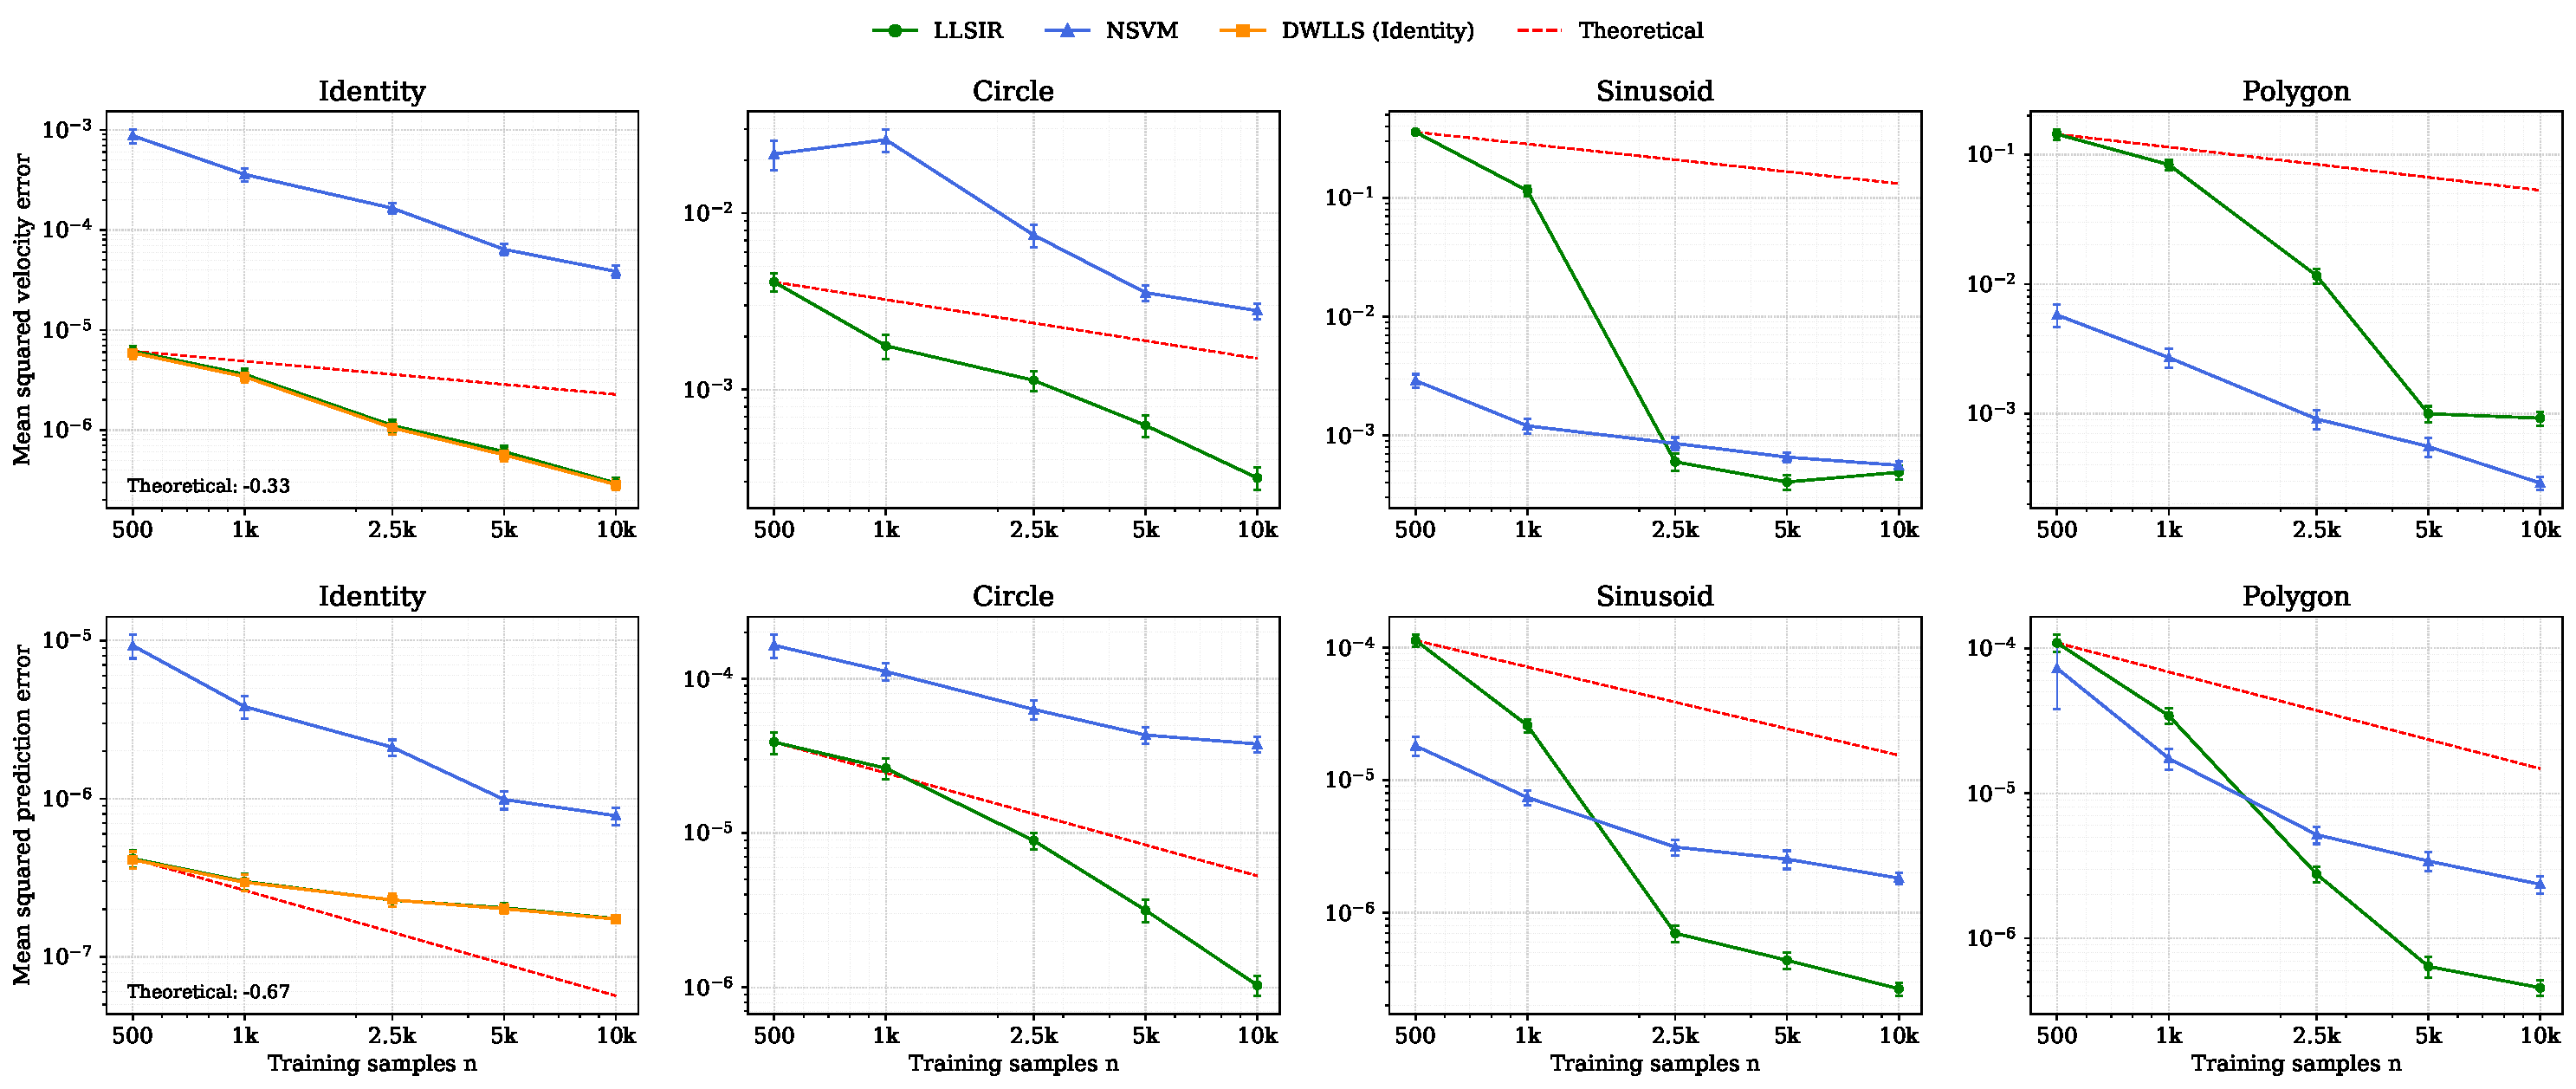
\includegraphics[width=\linewidth]{figures/error_fixed_point.pdf}
    \caption{Planar fixed-point experiment ($d=2$). The top row shows mean squared velocity error, using unit directions and the smaller error over the two possible signs; the bottom row shows mean squared prediction error. Columns correspond to Identity, Circle, Sinusoid, and Polygon. Each node averages $B=100$ nested training trials, and error bars show one Monte Carlo standard error. Red dashed lines indicate the theoretical guides.}
    \label{fig:fixed-point-planar}
\end{figure}

\begin{figure}[htbp]
    \centering
    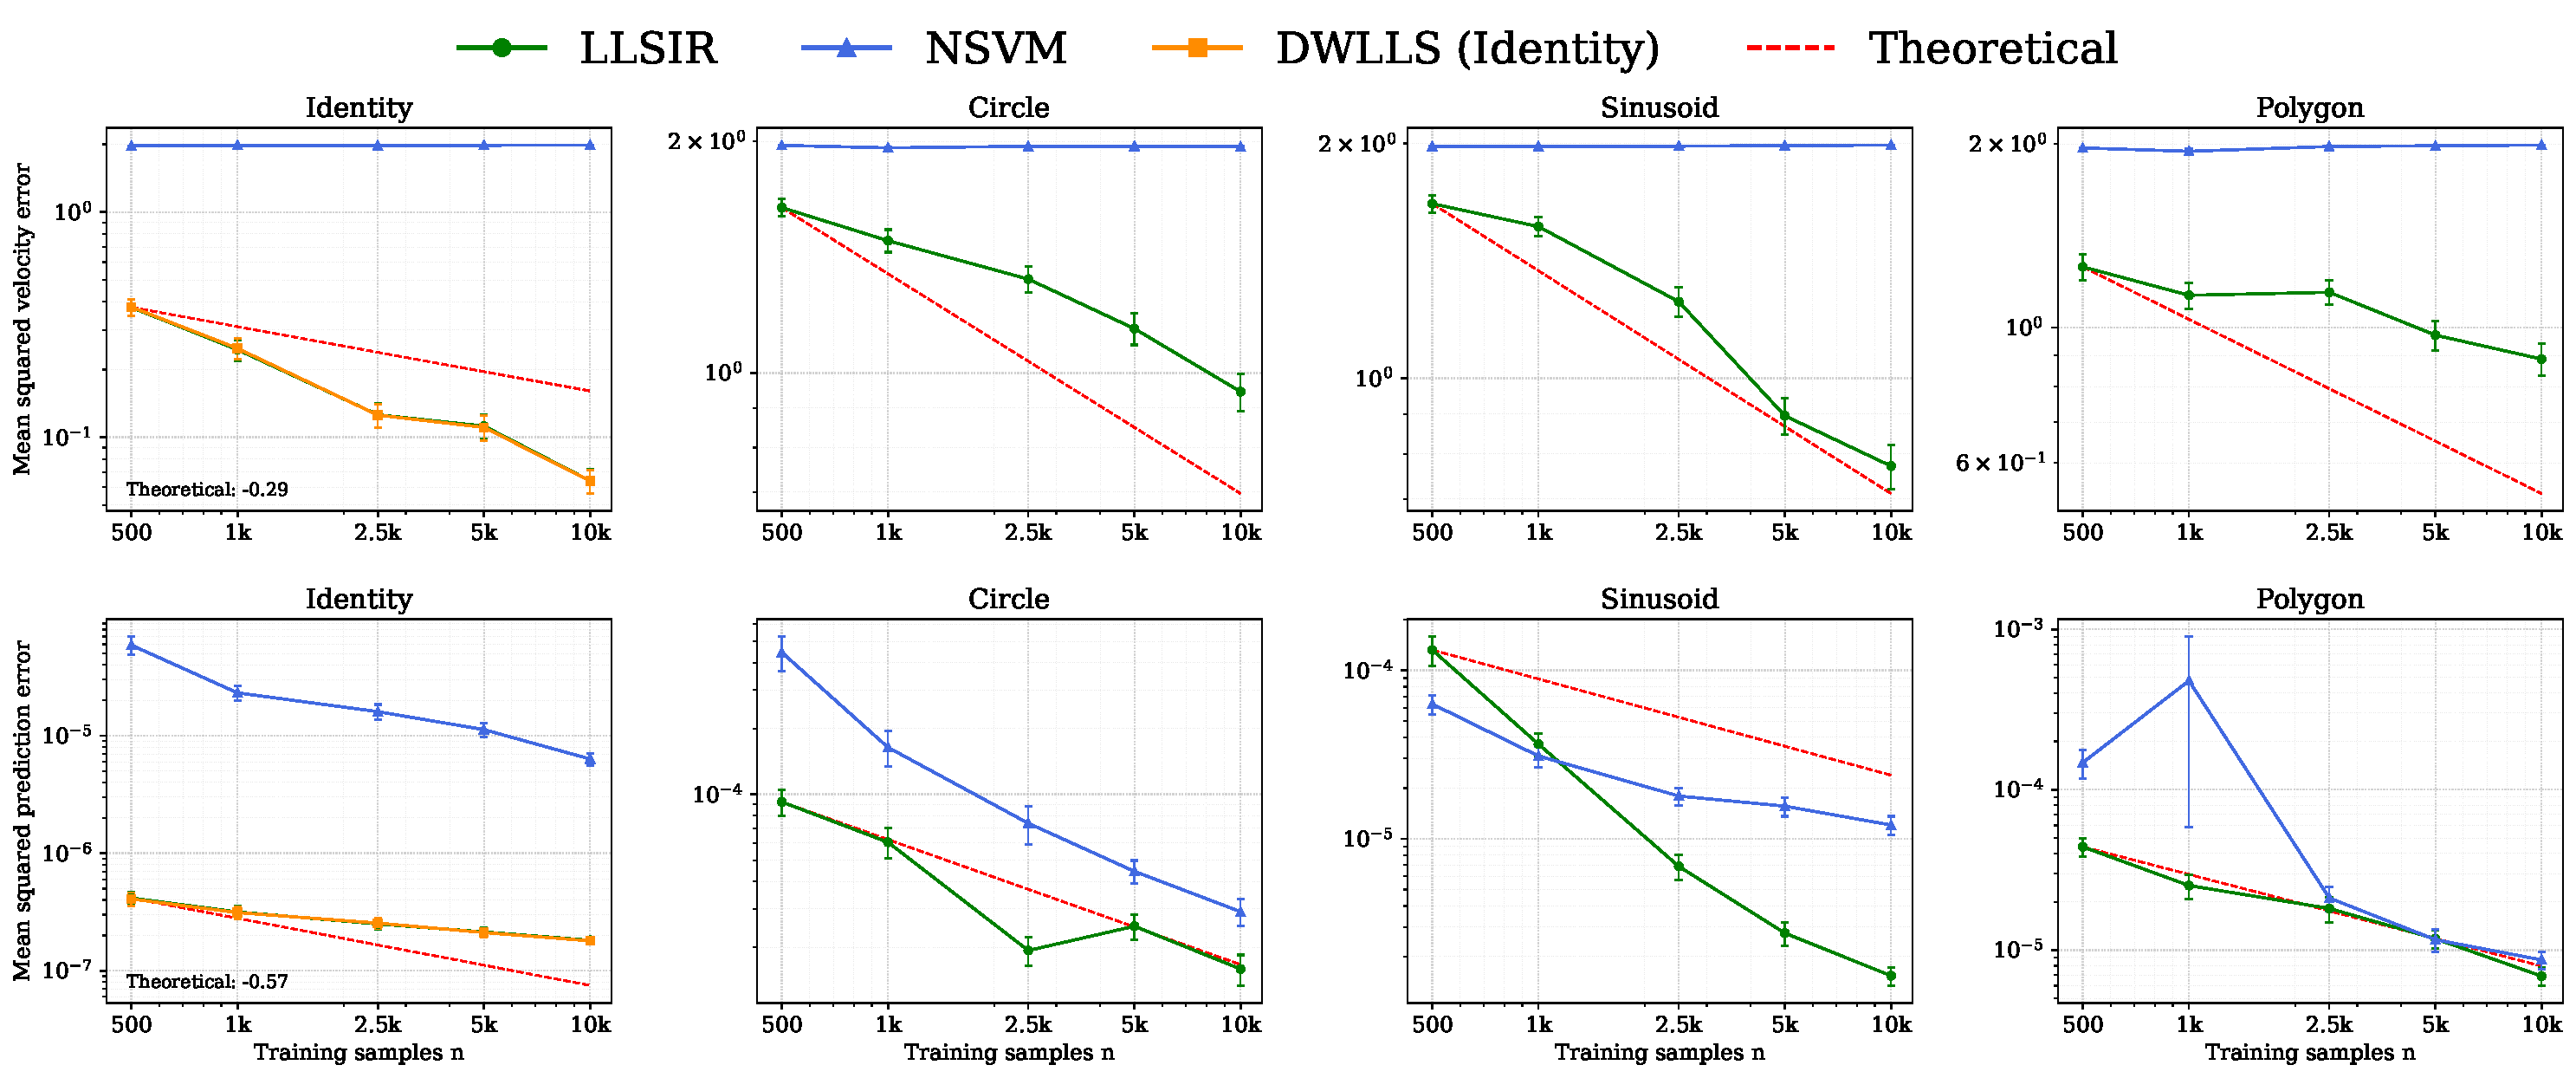
\includegraphics[width=\linewidth]{figures/error_lifted_fixed_point.pdf}
    \caption{Lifted fixed-point experiment ($d=3$), using the same design as \Cref{fig:fixed-point-planar}. The planar covariates are embedded in three dimensions and perturbed only in the third coordinate by independent $\mathcal{N}(0,10^{-6})$ noise (standard deviation $10^{-3}$). The curves and fixed inference locations remain at $z=0$. Velocity errors are measured in three dimensions; means and standard-error bars again use $B=100$ nested training trials.}
    \label{fig:fixed-point-lifted}
\end{figure}


\subsection{Asymptotic performance}

\begin{table*}[h]
\small
\centering
 \begin{tabular}{l | >{\centering\arraybackslash}p{0.15\textwidth}  >{\centering\arraybackslash}p{0.15\textwidth}  >{\centering\arraybackslash}p{0.15\textwidth} >{\centering\arraybackslash}p{0.15\textwidth} }
  \toprule  & Identity &  Circle & Sinusoid & Polygon \\
\midrule
 \hline
 $d = 2$ & $-0.85$ & $-0.48$ & $-1.53$ & $-0.10$ \\
 $d = 4$ & $-0.51$ & $-0.85$ & $-0.55$ & $-0.07$ \\
 $d = 6$ & $-0.45$ & $-0.11$ & $-0.56$ & $-0.23$ \\
 $d = 8$ & $-0.29$ & $-0.14$ & $-0.05$ & $-0.00$ \\
 $d = 10$ & $-0.14$ & $-0.13$ & $-0.13$ & $-0.02$ \\
\bottomrule
 \end{tabular}
 \caption{Log-log slope for velocity error (projection)}
 \label{tab:vel}
\end{table*}

\begin{table*}[h]
\small
\centering
 \begin{tabular}{l | >{\centering\arraybackslash}p{0.15\textwidth}  >{\centering\arraybackslash}p{0.15\textwidth}  >{\centering\arraybackslash}p{0.15\textwidth} >{\centering\arraybackslash}p{0.15\textwidth} }
  \toprule  & Identity &  Circle & Sinusoid & Polygon \\
\midrule
 \hline
 $d = 2$ & $-1.10$ & $-0.96$ & $-1.02$ & $-0.27$ \\
 $d = 4$ & $-0.65$ & $-0.59$ & $-1.03$ & $-0.24$ \\
 $d = 6$ & $-0.53$ & $-0.96$ & $-0.25$ & $-0.42$ \\
 $d = 8$ & $-0.46$ & $-0.48$ & $-0.06$ & $-0.00$ \\
 $d = 10$ & $-0.48$ & $-0.52$ & $-0.06$ & $-0.01$ \\
\bottomrule
 \end{tabular}
 \caption{Log-log slope for regression error (projection)}
 \label{tab:reg}
\end{table*}

\begin{table*}[h]
\small
\centering
 \begin{tabular}{l | >{\centering\arraybackslash}p{0.15\textwidth} >{\centering\arraybackslash}p{0.15\textwidth} >{\centering\arraybackslash}p{0.15\textwidth} }
  \toprule  & $\sin(\pi x_1)$ & $\|x\|^2$ & $x_1 x_2$ \\
\midrule
 \hline
 $d = 2$ & $-0.94$ & $-1.02$ & $-0.66$ \\
 $d = 4$ & $-0.82$ & $-0.84$ & $-0.55$ \\
 $d = 6$ & $-0.84$ & $-0.74$ & $-0.63$ \\
 $d = 8$ & $-0.64$ & $-0.39$ & $-0.45$ \\
 $d = 10$ & $-0.36$ & $-0.31$ & $-0.37$ \\
\bottomrule
 \end{tabular}
 \caption{Log-log slope for velocity error (general)}
 \label{tab:vel-general}
\end{table*}

\begin{table*}[h]
\small
\centering
 \begin{tabular}{l | >{\centering\arraybackslash}p{0.15\textwidth} >{\centering\arraybackslash}p{0.15\textwidth} >{\centering\arraybackslash}p{0.15\textwidth} }
  \toprule  & $\sin(\pi x_1)$ & $\|x\|^2$ & $x_1 x_2$ \\
\midrule
 \hline
 $d = 2$ & $-0.86$ & $-1.02$ & $-0.98$ \\
 $d = 4$ & $-0.60$ & $-0.66$ & $-0.61$ \\
 $d = 6$ & $-0.52$ & $-0.49$ & $-0.58$ \\
 $d = 8$ & $-0.32$ & $-0.37$ & $-0.40$ \\
 $d = 10$ & $-0.40$ & $-0.34$ & $-0.37$ \\
\bottomrule
 \end{tabular}
 \caption{Log-log slope for regression error (general)}
 \label{tab:reg-general}
\end{table*}

For the dimension-sweep experiments summarized in the tables, we generate data from the model $Y_i = f(g(X_i)) + \varepsilon_i$ with $f$ the identity link, $X_1, \dots, X_N \sim \mathcal{U}([0,1]^d)$, and $\varepsilon_i \sim \mathcal{N}(0, 0.01^2)$. We vary the ambient dimension over $d \in \{2, 4, 6, 8, 10\}$ and consider two families of index functions $g$ described below.

\paragraph{Experimental setup.} For every $(d, g)$ pair, we select five query points $x_0$ and set the base localization radius to $\varepsilon_0 = \max\bigl(\varepsilon_0^{\mathrm{model}},\, (50 / N_0 V_d)^{1/d}\bigr)$, where $V_d = \pi^{d/2} / \Gamma(d/2 + 1)$ is the volume of the unit ball in $\mathbb{R}^d$ and $N_0$ is the smallest sample size. For each sample size $N$, the radius is scaled to $\varepsilon(N) = \varepsilon_0 \,(N/N_0)^{-1/(d+4)}$ for velocity estimation and $\varepsilon(N) = \varepsilon_0\,(N/N_0)^{-1/(d+2)}$ for regression. We vary $N$ over six geometrically spaced values from 5K to 30K and run 50 independent Monte Carlo trials per configuration. For each trial we fit a least-squares line of $\log N$ against $\log \text{error}$ and record the slope.

\paragraph{Projection.} We first take $g = \Pi$, the closest-point projection onto a curve $\gamma \colon [0,1] \to \mathbb{R}^2$ embedded in $\mathbb{R}^d$ by setting the remaining $d - 2$ coordinates to zero. Concretely, $\Pi(x) = \arg\min_{t \in [0,1]} |x - \gamma(t)|$ returns the curve parameter of the nearest point. We consider four curves, (i) Identity, $\gamma(t) = (t,\, t)$, (ii) Circle, $\gamma(t) = (0.5 + 0.4\cos 2\pi t,\; 0.5 + 0.4\sin 2\pi t)$, (iii) Sinusoid, $\gamma(t) = (t,\; 0.5 + 0.4\sin 2\pi t)$, and (iv) Polygon, the piecewise-linear path joining $(0.15, 0.20) \to (0.85, 0.25) \to (0.75, 0.80) \to (0.35, 0.90) \to (0.10, 0.55)$, parametrized by arc length. To avoid discontinuity at the medial axis, we evaluate $|x_0 - \gamma(t)|$ on a grid of 5K values of $t$ and identify local minima corresponding to distinct curve segments separated by $\Delta_t \ge 0.1$ in parameter space, and if multiple segments are nearby, shrink the base radius $\varepsilon_0$ to $0.45(d_2 - d_1)$, where $d_1, d_2$ are the distances to the nearest and second-nearest segments. Tables~\ref{tab:vel} and~\ref{tab:reg} report the slope averaged over all 50 trials.

\paragraph{General.} We next take $g$ to be a smooth, explicitly defined function, for which no medial axis complications arise. The three choices are (i) $g(x) = \sin(\pi x_1)$, (ii) $g(x) = \|x\|^2$, and (iii) $g(x) = x_1 x_2$. Tables~\ref{tab:vel-general} and~\ref{tab:reg-general} report the slope averaged over all 50 trials.

\section{Proofs of key results}



\subsection{Proof of \Cref{thm: population prop}} \label{sec: proof of population vel prop}
It suffices to show that $\beta^*_{x_0, \epsilon} \rightarrow  \begin{bmatrix}c_0 &  c_*\nabla g(x_0)\end{bmatrix}$ up to scale where $c_0$ is some scalar. To show this, we'll define the \say{surrogate} target  
\[m(x) = f\Big(g(x_0) + \nabla g(x_0)^{\top}(x-x_0)\Big)\]
as described in \Cref{eq: surrogate decomposition colloquial} and the surrogate residual 
\[\xi(x) = f(g(x)) - m(x).\] Note that \Cref{lemma: proj approx general} implies that $ |\xi(x+x_0)| \leq C_{x_0}\|x\|_2^2$ for all $x\in\mathcal{B}(0,\epsilon)$. Let  
\begin{align}
    \tilde{\beta}^*_{x_0, \epsilon} &= \arg\min_{\beta}\mathbb{E}\Big[\mathbbm{1}_{\{x \in \mathcal{B}(0, \epsilon)\}}\frac{p^*(x)}{p_{0}(x)}\Big(m(x+x_0) - X^{\top}\beta\Big)^2\Big] \label{eq: perturbed pop estimator}
\end{align}
where the expectation is taken with respect to $x \sim p_{x}$. By \Cref{lemma: surrogate problem} we know that for some $c_0, c_* \in \mathbb{R}$ we have $\tilde{\beta}^*_{x_0, \epsilon}  =  \begin{bmatrix}
    c_0 & c_*\nabla g(x_0)
\end{bmatrix}^{\top}$, while \Cref{lemma: constant of prop} gives the exact characterization $c_* = \epsilon f'(g(x_0))+ o(\epsilon^2)$. Observe that $\mathbb{E}[wXX^{\top}]$ is positive definite by \Cref{lemma: pd}. Thus, \Cref{lemma: perturbation} and \Cref{beta tilde simplification} give
\[
    v^*_{x_0,\epsilon}-V\tilde{\beta}_{x_0,\epsilon}^*
    =
    VQ^{-1}\mathbb{E}[wX\xi(x+x_0)]
    =
    \frac{\epsilon}{\nu_\epsilon^2}
    \mathbb{E}_{p^*}\left[
    \mathbbm{1}_{\{x\in\mathcal{B}(0,\epsilon)\}}
    x\xi(x+x_0)
    \right],
\]
where $\nu_\epsilon^2=\mathbb{E}_{p^*}[\mathbbm{1}_{\{x\in\mathcal{B}(0,\epsilon)\}}x_1^2]$. Taking norms and using the bound on $\xi$ gives
\begin{align*}
    \|v^*_{x_0,\epsilon}-V\tilde{\beta}_{x_0,\epsilon}^*\|_2
    &\leq
    \frac{C_{x_0}\epsilon}{\nu_\epsilon^2}
    \mathbb{E}_{p^*}\left[
    \mathbbm{1}_{\{x\in\mathcal{B}(0,\epsilon)\}}
    \|x\|_2^3
    \right] \\
    &\leq
    \frac{C_{x_0}\epsilon^2}{\nu_\epsilon^2}
    \mathbb{E}_{p^*}\left[
    \mathbbm{1}_{\{x\in\mathcal{B}(0,\epsilon)\}}
    \|x\|_2^2
    \right] \\
    &= C_{x_0}d\epsilon^2.
\end{align*}
\qed{}


\subsection{Proof of \Cref{thm: decomposition for beta}} \label{sec: proof of velocity decomp}
% This proof will follow closely the argument from \citet{Newey_Ruud_2005}. Let's define the matrices
% \begin{equation*}
%     Q = \mathbb{E}_{p_{x}}\left[wXX^{\top}\right] \qquad \text{and} \qquad \hat{Q} = \frac{1}{n}\sum_{i = 1}^n\hat{w}_iX_iX_i^{\top}.
% \end{equation*}
% We have
% \begin{align*}
%     \hat{v}_{x_0, \epsilon} - v^*_{x_0, \epsilon} &= V\hat{Q}^{-1}\left(\frac{1}{n}\sum_{i = 1}^n\hat{w}_iX_iy_i\right) - \beta^*_{x_0, \epsilon} \\
%     &= V\hat{Q}^{-1}\left(\frac{1}{n}\sum_{i = 1}^n\hat{w}_iX_iy_i - \hat{Q}\beta^*_{x_0, \epsilon}\right) \\
%     &= V\hat{Q}^{-1}\left(\frac{1}{n}\sum_{i = 1}^n\hat{w}_iX_i\underbrace{\left(y_i - X_i^{\top}\beta^*_{x_0, \epsilon}\right)}_{u_i}\right) \\
%     &= V\hat{Q}^{-1}\left(\frac{1}{n}\sum_{i = 1}^n\hat{w}_iX_iu_i\right).
% \end{align*}
% Now we'll add and subtract out a term with the true weights $w_i$ to obtain
% \begin{align*}
%     \hat{v}_{x_0, \epsilon} - v^*_{x_0, \epsilon} &= V\hat{Q}^{-1}\left(\frac{1}{n}\sum_{i = 1}^nw_iX_iu_i + \frac{1}{n}\sum_{i = 1}^n(\hat{w}_i - w_i)X_iu_i\right) \\
%     &= V\hat{Q}^{-1}\Bigg(\frac{1}{n}\sum_{i = 1}^n\frac{\mathbbm{1}_{\{x_i \in \mathcal{B}(0, \epsilon)\}}p^*(x_i)X_iu_i}{p_{x}(x_i)} \\
%     &\hspace{40mm}+ \frac{1}{n}\sum_{i = 1}^n\left[\frac{1}{\hat{p}_{x}(x_i)} - \frac{1}{p_{x}(x_i)}\right]\mathbbm{1}_{\{x_i \in \mathcal{B}(0, \epsilon)\}}p^*(x_i)X_iu_i\Bigg).
% \end{align*}
% Now if we define $a(z) = \mathbbm{1}_{\{x_i \in \mathcal{B}(0, \epsilon)\}}p^*(x_i)X_iu_i$ then we can write the above expression as
% \begin{align*}
%     \hat{v}_{x_0, \epsilon} - v^*_{x_0, \epsilon} &= V\hat{Q}^{-1}\left(\frac{1}{n}\sum_{i = 1}^n\frac{a(z)}{p_{x}(x_i)} + \frac{1}{n}\sum_{i = 1}^n\left[\frac{1}{\hat{p}_{x}(x_i)} - \frac{1}{p_{x}(x_i)}\right]a(z)\right).
% \end{align*}
% Now we'll apply a first order Taylor expansion of $g(t) = 1/t$ where $\Delta(x_i) = \hat{p}_{x}(x_i) - p_{x}(x_i)$ to say,
% \begin{align}
%     \hat{v}_{x_0, \epsilon} - v^*_{x_0, \epsilon} &= V\hat{Q}^{-1}\bigg(\frac{1}{n}\sum_{i = 1}^n\frac{a(z)}{p_{x}(x_i)} - \underbrace{\frac{1}{n}\sum_{i = 1}^n\frac{a(z)\Delta(x_i)}{p_{x}^2(x_i)}}_{R_1} + \underbrace{\frac{1}{n}\sum_{i = 1}^na(z) \frac{1}{2}g''(\xi_i)\Delta(x_i)^2}_{R_2}\bigg) \label{eq: expansion with remainder}
% \end{align}
% where $\xi_i$ is some value between $p_{x}(x_i)$ and $\hat{p}_{x}(x_i)$. Now note that $\mathbb{E}[a(z)/p_{x}(x)] = \mathbb{E}[wXu] = 0$ by the population first order conditions. We'll adopt the notation that $\mathbb{P}f = \mathbb{E}_{p_{x}}[f]$ and $\mathbb{P}_nf = \frac{1}{n}\sum_{i = 1}^nf(x_i)$. Thus,
% \begin{align*}
%     \frac{1}{n}\sum_{i = 1}^n\frac{a(z)}{p_{x}(x_i)} &= \frac{1}{n}\sum_{i = 1}^n\frac{a(z)}{p_{x}(x_i)} - \mathbb{E}\left[\frac{a(z)}{p_{x}(x)}\right] \\
%     &= (\mathbb{P}_n -\mathbb{P})\left[\frac{a(z)}{p_{x}(x)}\right] \\
%     &= \frac{1}{n}\sum_{i = 1}^n w_i X_i u_i.
% \end{align*}
% Now we'll consider the first remainder term. By \Cref{lemma: remainder term}
% \[R_1 = \frac{1}{n}\sum_{i = 1}^n \frac{\mathbb{E}[a(Z)\,| \,x_i]}{p_{x}(x_i)} + O_p\left( \epsilon^dh^s + \sqrt{\frac{\epsilon^d}{n^2h^d}}\right).\]
% Note that \Cref{lemma: uniform convergence of kde} indicates that \[\sup_{x\in \mathcal{B}(0, \epsilon)} \left|\Delta(x)\right| =O_p\left(\sqrt{\frac{\log n}{nh^d}} +h^s \right) =o_p(1)\] when $h \rightarrow 0$ and $nh^d \rightarrow \infty$. Thus, 
% \begin{align*}
%     \|R_2\|_2 &= \left\|\mathbb{P}_n\left[\frac{a(z)}{p_{x}(x)}p_{x}(x)\frac{1}{2}g''(\xi)\Delta(x)^2\right]\right\|_2\\
%     &\leq \mathbb{P}_n[\left\|wXu\right\|_2(1/2)|g''(\xi)|]\sup_{\mathcal{B}(0, \epsilon)}|p_{x}(x)|\cdot \sup_{\mathcal{B}(0, \epsilon)}|\Delta(x)|^2. 
% \end{align*}
% Now note that $g''(t) = 2/t^3$  -- since $\sup_{x\in \mathcal{B}(0, \epsilon)} \left|\Delta(x)\right| = o_p(1)$ we know that $\hat{p}_{x} > m/2$ for all $x \in \mathcal{B}(0, \epsilon)$ with probability approaching $1$. It follows that $\xi_i > m/2$ with probability approaching $1$ as well. Thus,
% \begin{align*}
%     \|R_2\|_2 &\leq \mathbb{P}_n\left\|wXu\right\|_2\cdot (8/m^3)\cdot \sup_{\mathcal{B}(0, \epsilon)}|p_{x}(x)|\cdot \sup_{\mathcal{B}(0, \epsilon)}|\Delta(x)|^2 \\
%     &= \mathbb{P}_n\left\|wXu\right\|_2 \cdot O_p\left(\frac{\log n}{nh^d} +h^{2s} \right) \\
%     &= O_p\left(\frac{\epsilon^d\log n}{nh^d} +\epsilon^dh^{2s}\right) 
% \end{align*}
% with probability approaching $1$. Writing $\mathfrak R_n := \frac{\epsilon^d\log n}{nh^d} +\epsilon^dh^{2s}$, we have
% \begin{align*}
%     \hat{v}_{x_0, \epsilon} - v^*_{x_0, \epsilon} &= V\hat{Q}^{-1}\left(\frac{1}{n}\sum_{i = 1}^n\frac{a(z_i) - \mathbb{E}[a(Z)\,|\, x_i]}{p_{x}(x_i)} + O(\epsilon^dh^s) + O_p\left( \mathfrak R_n + \sqrt{\frac{\epsilon^d}{n^2h^d}}\right)\right).
% \end{align*}
% Now we will introduce $Q$ as follows,
% \begin{equation*}
%     \hat{v}_{x_0, \epsilon} - v^*_{x_0, \epsilon} = VQ^{-1}\psi_n + V(\hat{Q}^{-1} - Q^{-1})\psi_n
% \end{equation*}
% with
% \begin{align*}
%     \psi_n &= \frac{1}{n}\sum_{i = 1}^n\frac{a(z_i) -\mathbb{E}[a(Z)\,|\, x_i]}{p_{x}(x_i)} +    \underbrace{O(\epsilon^dh^s) + O_p\left( \mathfrak R_n +  \sqrt{\frac{\epsilon^d}{n^2h^d}}\right)}_{:= r_n} \\
%     &= O_p\left(\sqrt{\frac{\epsilon^d}{n}}+\mathfrak R_n + \epsilon^dh^s + \sqrt{\frac{\epsilon^d}{n^2h^d}}\right).
% \end{align*}
% By \Cref{lemma: Q convergence} we know that 
% \[\|\hat{Q}^{-1} - Q^{-1}\|_{\operatorname{op}} = O_p\left(\frac{1}{\epsilon^{3d/2}\sqrt{n}} + \frac{1}{n\epsilon^{2d}}\right) + o_p\left(\frac{1}{\epsilon^d}\right) = o_p(\epsilon^{-d})\]
% under our standing assumptions on the parameters. It follows that 
% \[
% (\hat Q^{-1}-Q^{-1})\psi_n
% =
% o_p\left(
% \frac1{\sqrt{n\epsilon^d}}
% +
% h^s
% +
% \frac{\log n}{nh^d}
% +
% h^{2s}
% +
% \frac1{nh^{d/2}\epsilon^{d/2}}
% \right) = o_p\left(
% \frac1{\sqrt{n\epsilon^d}}\right)
% \]
% when $h \asymp n^{-1/(2s+d)}$ and $\sqrt{n\epsilon^d}n^{-s/(2s+d)} \rightarrow 0$. Furthermore, $\|Q^{-1}\|_{\operatorname{op}} \lesssim \epsilon^{-d}$ as derived in \Cref{lemma: Q op norm}. Thus,
% \begin{align*}
%     \|Q^{-1}r_n\|_2 &\leq \|Q^{-1}\|_{\operatorname{op}}\|r_n\|_2 \\
%     &= O(\epsilon^{-d})O_p\left( \mathfrak R_n + \epsilon^dh^s + \sqrt{\frac{\epsilon^d}{n^2h^d}}\right) \\
%     &= o_p\left(\frac{1}{\sqrt{n\epsilon^d}}\right).
% \end{align*}
% Putting it together, we obtain
% \begin{equation}
%     \hat{v}_{x_0, \epsilon} - v^*_{x_0, \epsilon} = \frac{1}{n}VQ^{-1}\sum_{i = 1}^n w_iX_i(u_i - \mathbb{E}[u_i\,|\,X_i]) \\
%     +  o_p\left(\frac{1}{\sqrt{n\epsilon^{d}}}\right).
% \end{equation}
% \qed{}

This proof will follow closely the argument from \citet{Newey_Ruud_2005}. Let's define the matrices
\begin{equation*}
    Q = \mathbb{E}_{p_{x}}\left[wXX^{\top}\right] \qquad \text{and} \qquad \hat{Q} = \frac{1}{n}\sum_{i = 1}^n\hat{w}_iX_iX_i^{\top}.
\end{equation*}
We have
\begin{align*}
    \hat{v}_{x_0, \epsilon} - v^*_{x_0, \epsilon} &= V\hat{Q}^{-1}\left(\frac{1}{n}\sum_{i = 1}^n\hat{w}_iX_iy_i\right) - V\beta^*_{x_0, \epsilon} \\
    &= V\hat{Q}^{-1}\left(\frac{1}{n}\sum_{i = 1}^n\hat{w}_iX_iy_i - \hat{Q}\beta^*_{x_0, \epsilon}\right) \\
    &= V\hat{Q}^{-1}\left(\frac{1}{n}\sum_{i = 1}^n\hat{w}_iX_i\underbrace{\left(y_i - X_i^{\top}\beta^*_{x_0, \epsilon}\right)}_{u_i}\right) \\
    &= V\hat{Q}^{-1}\left(\frac{1}{n}\sum_{i = 1}^n\hat{w}_iX_iu_i\right).
\end{align*}
Now we'll add and subtract out a term with the true weights $w_i$ to obtain
\begin{align*}
    \hat{v}_{x_0, \epsilon} - v^*_{x_0, \epsilon} &= V\hat{Q}^{-1}\left(\frac{1}{n}\sum_{i = 1}^nw_iX_iu_i + \frac{1}{n}\sum_{i = 1}^n(\hat{w}_i - w_i)X_iu_i\right) \\
    &= V\hat{Q}^{-1}\Bigg(\frac{1}{n}\sum_{i = 1}^n\frac{\mathbbm{1}_{\{x_i \in \mathcal{B}(0, \epsilon)\}}p^*(x_i)X_iu_i}{p_{x}(x_i)} \\
    &\hspace{40mm}+ \frac{1}{n}\sum_{i = 1}^n\left[\frac{1}{\hat{p}_{x}(x_i)} - \frac{1}{p_{x}(x_i)}\right]\mathbbm{1}_{\{x_i \in \mathcal{B}(0, \epsilon)\}}p^*(x_i)X_iu_i\Bigg).
\end{align*}
Now if we define $a(z_i) = \mathbbm{1}_{\{x_i \in \mathcal{B}(0, \epsilon)\}}p^*(x_i)X_iu_i$ then we can write the above expression as
\begin{align*}
    \hat{v}_{x_0, \epsilon} - v^*_{x_0, \epsilon} &= V\hat{Q}^{-1}\left(\frac{1}{n}\sum_{i = 1}^n\frac{a(z_i)}{p_{x}(x_i)} + \frac{1}{n}\sum_{i = 1}^n\left[\frac{1}{\hat{p}_{x}(x_i)} - \frac{1}{p_{x}(x_i)}\right]a(z_i)\right).
\end{align*}
Now we'll apply a first order Taylor expansion of $g(t) = 1/t$ where $\Delta(x_i) = \hat{p}_{x}(x_i) - p_{x}(x_i)$ to say,
\begin{align}
    \hat{v}_{x_0, \epsilon} - v^*_{x_0, \epsilon} &= V\hat{Q}^{-1}\bigg(\frac{1}{n}\sum_{i = 1}^n\frac{a(z_i)}{p_{x}(x_i)} - \underbrace{\frac{1}{n}\sum_{i = 1}^n\frac{a(z_i)\Delta(x_i)}{p_{x}^2(x_i)}}_{R_1} + \underbrace{\frac{1}{n}\sum_{i = 1}^na(z_i) \frac{1}{2}g''(\xi_i)\Delta(x_i)^2}_{R_2}\bigg) \label{eq: expansion with remainder}
\end{align}
where $\xi_i$ is some value between $p_{x}(x_i)$ and $\hat{p}_{x}(x_i)$. Now note that $\mathbb{E}[a(Z)/p_{x}(X)] = \mathbb{E}[wXu] = 0$ by the population first order conditions. We'll adopt the notation that $\mathbb{P}f = \mathbb{E}_{p_{x}}[f]$ and $\mathbb{P}_nf = \frac{1}{n}\sum_{i = 1}^nf(x_i)$. Thus,
\begin{align*}
    \frac{1}{n}\sum_{i = 1}^n\frac{a(z_i)}{p_{x}(x_i)} &= \frac{1}{n}\sum_{i = 1}^n\frac{a(z_i)}{p_{x}(x_i)} - \mathbb{E}\left[\frac{a(Z)}{p_{x}(X)}\right] \\
    &= (\mathbb{P}_n -\mathbb{P})\left[\frac{a(Z)}{p_{x}(X)}\right] \\
    &= \frac{1}{n}\sum_{i = 1}^n w_i X_i u_i.
\end{align*}
Now we'll consider the first remainder term. By \Cref{lemma: remainder term},
\[
    R_1 = \frac{1}{n}\sum_{i = 1}^n \frac{\mathbb{E}[a(Z)\,|\,X=x_i]}{p_{x}(x_i)} + o_p\left(\sqrt{\frac{\epsilon^d}{n}}\right).
\]
For the second remainder term, \Cref{lemma: uniform convergence of kde} and the standing choice $h\asymp n^{-1/(2s+d)}$ imply
\[
    \sup_{x\in \mathcal{B}(0, \epsilon)} \left|\Delta(x)\right| =O_p\left(\sqrt{\frac{\log n}{nh^d}} +h^s \right) =o_p(1),
\]
where $nh^d/\log n\rightarrow\infty$. Thus,
\begin{align*}
    \|R_2\|_2 &= \left\|\mathbb{P}_n\left[\frac{a(Z)}{p_{x}(X)}p_{x}(X)\frac{1}{2}g''(\xi)\Delta(X)^2\right]\right\|_2\\
    &\leq \mathbb{P}_n[\left\|wXu\right\|_2(1/2)|g''(\xi)|]\sup_{\mathcal{B}(0, \epsilon)}|p_{x}(x)|\cdot \sup_{\mathcal{B}(0, \epsilon)}|\Delta(x)|^2.
\end{align*}
Now note that $g''(t) = 2/t^3$. Since $p_{x}\geq m>0$ on $\mathcal{B}(0,\epsilon)$ and $\sup_{x\in \mathcal{B}(0,\epsilon)}|\Delta(x)|=o_p(1)$, we know that $\hat{p}_{x}(x)>m/2$ uniformly on $\mathcal{B}(0,\epsilon)$ with probability approaching $1$. It follows that $\xi_i>m/2$ with probability approaching $1$ as well. Moreover, the standing moment assumptions and local boundedness of the density ratio imply $\mathbb{E}\|wXu\|_2=O(\epsilon^d)$, and hence $\mathbb{P}_n\|wXu\|_2=O_p(\epsilon^d)$. Therefore,
\begin{align*}
    \|R_2\|_2 &\leq \mathbb{P}_n\left\|wXu\right\|_2\cdot (8/m^3)\cdot \sup_{\mathcal{B}(0, \epsilon)}|p_{x}(x)|\cdot \sup_{\mathcal{B}(0, \epsilon)}|\Delta(x)|^2 \\
    &= O_p\left(\epsilon^d\left\{\frac{\log n}{nh^d} +h^{2s}\right\}\right) \\
    &= o_p\left(\sqrt{\frac{\epsilon^d}{n}}\right),
\end{align*}
where the final line follows from $h\asymp n^{-1/(2s+d)}$ and $\epsilon/h\rightarrow0$. Indeed, $nh^{2s+d}\asymp1$, so
\[
    \frac{\epsilon^d h^{2s}(1+\log n)}{\sqrt{\epsilon^d/n}}
    \asymp
    \left(\frac{\epsilon}{h}\right)^{d/2}h^s(1+\log n)
    \rightarrow0.
\] Combining the bounds for $R_1$ and $R_2$ in \cref{eq: expansion with remainder} gives
\begin{align*}
    \hat{v}_{x_0, \epsilon} - v^*_{x_0, \epsilon}
    &= V\hat{Q}^{-1}\left(\frac{1}{n}\sum_{i = 1}^n\frac{a(z_i) - \mathbb{E}[a(Z)\,|\,X=x_i]}{p_{x}(x_i)}
    + o_p\left(\sqrt{\frac{\epsilon^d}{n}}\right)\right).
\end{align*}
Now we will introduce $Q$ as follows,
\begin{equation*}
    \hat{v}_{x_0, \epsilon} - v^*_{x_0, \epsilon} = VQ^{-1}\psi_n + V(\hat{Q}^{-1} - Q^{-1})\psi_n
\end{equation*}
with
\begin{align*}
    \psi_n &= \frac{1}{n}\sum_{i = 1}^n\frac{a(z_i) -\mathbb{E}[a(Z)\,|\,X=x_i]}{p_{x}(x_i)}
    + o_p\left(\sqrt{\frac{\epsilon^d}{n}}\right) \\
    &= O_p\left(\sqrt{\frac{\epsilon^d}{n}}\right).
\end{align*}
Indeed, the summands in the first term are mean zero and the standing moment and density assumptions imply
$\mathbb{E}\|(a(Z)-\mathbb{E}[a(Z)\mid X])/p_{x}(X)\|_2^2=O(\epsilon^d)$. By \Cref{lemma: Q convergence} we know that
\[
    \|\hat{Q}^{-1} - Q^{-1}\|_{\operatorname{op}}
    =
    O_p\left(\frac{1}{\epsilon^{3d/2}\sqrt{n}} + \frac{1}{n\epsilon^{2d}}\right) + o_p\left(\frac{1}{\epsilon^d}\right)
    =
    o_p(\epsilon^{-d})
\]
under our standing assumptions on the parameters. It follows that
\[
    \|(\hat Q^{-1}-Q^{-1})\psi_n\|_2
    =
    o_p(\epsilon^{-d})O_p\left(\sqrt{\frac{\epsilon^d}{n}}\right)
    =
    o_p\left(\frac{1}{\sqrt{n\epsilon^d}}\right).
\]
Furthermore, $\|Q^{-1}\|_{\operatorname{op}} \lesssim \epsilon^{-d}$ as derived in \Cref{lemma: Q op norm}, so
\[
    Q^{-1}o_p\left(\sqrt{\frac{\epsilon^d}{n}}\right)
    =
    o_p\left(\frac{1}{\sqrt{n\epsilon^d}}\right).
\]
Finally, observe that
\[
    \frac{a(z_i)-\mathbb{E}[a(Z)\mid X=x_i]}{p_{x}(x_i)}
    =
    w_iX_i\left(u_i-\mathbb{E}[u_i\mid X_i]\right).
\]
Putting everything together, we obtain
\begin{equation}
    \hat{v}_{x_0, \epsilon} - v^*_{x_0, \epsilon}
    =
    \frac{1}{n}VQ^{-1}\sum_{i = 1}^nw_iX_i(u_i - \mathbb{E}[u_i\,|\,X_i])
    + o_p\left(\frac{1}{\sqrt{n\epsilon^{d}}}\right).
\end{equation}
\qed{}



\subsection{Proof of \Cref{corr: central limit for v}} \label{sec: proof of central limit for v}
From \Cref{thm: decomposition for beta} we have, 
\begin{align*}
    \hat{v}_{x_0, \epsilon} - v^*_{x_0, \epsilon} = \frac{1}{n}VQ^{-1}\sum_{i = 1}^nw_iX_i(u_i - \mathbb{E}[u_i|X_i]) 
    + O_p\left(h^s\right) + o_p\left(\frac{1}{\sqrt{n\epsilon^d}}\right).
\end{align*}
Multiplying through by $\sqrt{n\epsilon^{d}}$ yields
\begin{align*}
    \sqrt{n\epsilon^{d}}(\hat{v}_{x_0, \epsilon} - v^*_{x_0, \epsilon}) = \sqrt{\frac{\epsilon^{d}}{n}}VQ^{-1}\sum_{i = 1}^nw_iX_i(u_i - \mathbb{E}[u_i|X_i]) 
    + o_p\left(1\right)
\end{align*}
under the assymption that $\epsilon/h \to 0.$ Now we'll appeal to the Lyapunov central limit theorem described in \Cref{thm: lyapunov clt}. To do this, we will define the triangular array
\[U_{n, i} = \sqrt{\frac{\epsilon^{d}}{n}}VQ^{-1}w_iX_i(u_i - \mathbb{E}[u_i|X_i]).\]
Now let
\[
    V_n = \sum_{i=1}^n\operatorname{Cov}(U_{n,i})
    \qquad\text{and}\qquad
    v_n^2 = \lambda_{\min}(V_n).
\]
Since the $U_{n,i}$ are independent and identically distributed for each fixed $n$,
\begin{align*}
    V_n
    &= \frac{\epsilon^d}{n}\sum_{i=1}^n
    VQ^{-1}\operatorname{Cov}\left(w_iX_i(u_i-\mathbb{E}[u_i\mid X_i])\right)Q^{-1}V^\top \\
    &= \epsilon^dVQ^{-1}\Lambda Q^{-1}V^\top,
\end{align*}
where $\Lambda=\operatorname{Cov}(wX(u-\mathbb{E}[u\mid X]))$. By \Cref{lemma: asymptotic var bound},
\[
    V_n \rightarrow c_{\Sigma}I_d,
    \qquad
    c_{\Sigma}
    =
    \frac{(d+2)\sigma^2(0)}
    {p_{x}(0)\mathcal{L}(\mathcal{B}(0,1))}
    >0.
\]
Therefore, $v_n^2\rightarrow c_{\Sigma}$ and in particular $v_n$ is bounded away from zero for all sufficiently large $n$.

We now verify the Lyapunov condition in \Cref{thm: lyapunov clt} with $\delta=1$. We have
\begin{align*}
    \frac{1}{v_n^3}\sum_{i=1}^n\mathbb{E}\|U_{n,i}\|_2^3
    &=
    \frac{\epsilon^{3d/2}}{v_n^3\sqrt{n}}
    \mathbb{E}\left\|VQ^{-1}wX(u-\mathbb{E}[u\mid X])\right\|_2^3 \\
    &\leq
    \frac{\epsilon^{3d/2}}{v_n^3\sqrt{n}}
    \|VQ^{-1}\|_{\operatorname{op}}^3
    \mathbb{E}\left\|wX(u-\mathbb{E}[u\mid X])\right\|_2^3.
\end{align*}
By \Cref{lemma: Q op norm}, $\|Q^{-1}\|_{\operatorname{op}}\lesssim\epsilon^{-d}$. Moreover, $u-\mathbb{E}[u\mid X]=\varepsilon$, since conditional on $X$ we have $\mathbb{E}[u\mid X]=f(g(x))-X^\top\beta^*_{x_0,\epsilon}$. Thus, using $\|X\|_2\leq\sqrt{2}$ on $\mathcal{B}(0,\epsilon)$,
\begin{align*}
    \mathbb{E}\|wX(u-\mathbb{E}[u\mid X])\|_2^3
    &= \mathbb{E}\left[w^3\|X\|_2^3|\varepsilon|^3\right] \\
    &\leq 2^{3/2}w_{\max}^2\mathbb{E}\left[w|\varepsilon|^3\right] \\
    &= 2^{3/2}w_{\max}^2\int_{\mathcal{B}(0,\epsilon)}
    p^*(x)\mathbb{E}[|\varepsilon|^3\mid x]\,dx \\
    &\lesssim \epsilon^d.
\end{align*}
It follows that
\begin{align*}
    \frac{1}{v_n^3}\sum_{i=1}^n\mathbb{E}\|U_{n,i}\|_2^3
    &\lesssim
    \frac{\epsilon^{3d/2}}{v_n^3\sqrt{n}}
    \epsilon^{-3d}\epsilon^d \\
    &=
    \frac{1}{v_n^3\sqrt{n\epsilon^d}}
    =o(1),
\end{align*}
since $n\epsilon^d\rightarrow\infty$ and $v_n$ is bounded away from zero. Thus, \Cref{thm: lyapunov clt} applies and yields the theorem statement.

\qed{}

\subsection{Proof of \Cref{thm: regression ptwise decomp}} \label{sec: proof of reg decomp}

Without loss of generality, suppose that the $x_i$'s have been shifted so that $x_0 = 0$. Let $z_i = \langle x_i, v'^*_{x, \epsilon}\rangle$ and define
\begin{equation}
\tilde{f}(x_0) = \frac{\sum_{i=1}^n \mathbbm{1}_{\{x_i\in \mathcal{B}(0, \epsilon)\}}y_iK_r(\frac{z_i}{h_r})}{\sum_{i=1}^n \mathbbm{1}_{\{x_i\in \mathcal{B}(0, \epsilon)\}}K_r(\frac{z_i}{h_r})} \label{eq: ftilde}
\end{equation}
and
\begin{equation}\bar{f}(x_0) = \frac{\mathbb{E}\left[f(g(x))K_r(z/h_r)\mathbbm{1}_{\{x\in \mathcal{B}(0, \epsilon)\}}\right]}{\mathbb{E}\left[K_r(z/h_r)\mathbbm{1}_{\{x\in \mathcal{B}(0, \epsilon)\}}\right]}. \label{eq: fbar}
\end{equation}
 Expanding the difference $\hat{f}(x_0) - f(s_0)$ yields
\begin{align}
    \hat{f}(x) - f(s_0) &= \hat{f}(x_0) - \tilde{f}(x_0) + 
    \tilde{f}(x_0) - \bar{f}(x_0) + \bar{f}(x_0) - f(s_0).
\end{align}
By \Cref{lemma: fhat minus ftilde} we have
\begin{align}
    \hat{f}(x_0) - \tilde{f}(x_0) = \frac{1}{n}\sum_{j = 1}^n\langle\mu_{\psi}, \varphi_{\epsilon, j}\rangle + o_p\left(\frac{1}{\sqrt{n\epsilon^d}}\right)
\end{align}
where $\mu_{\psi} = \mathbb{E}[\psi_{\epsilon}]$,  
\[
\varphi_{\epsilon,j}
=
\frac{1}{\epsilon |f'(g(x_0))|\|\nabla g(x_0)\|_2}
P_{\epsilon}VQ^{-1}w_jX_j\left(u_j-\mathbb{E}[u_j\mid X_j]\right).
\]
and
\[\psi_{\epsilon, i} = \frac{\mathbbm{1}_{\{x_i \in \mathcal{B}(0, \epsilon)\}}(y_i - \bar{f}(x_0))\partial_{z_i}K_r(\frac{z_i}{h_r})x_i}{\mathbb{E}\left[\mathbbm{1}_{\{x \in \mathcal{B}(0, \epsilon)\}}K_r(z/h_r)\right]}.\]
Now \Cref{lemma: ftilde minus fbar} applies a similar decomposition to obtain an expression for $\tilde{f}(x) - \bar{f}(x)$. In particular,
\begin{align*}
    \tilde{f}(x) - \bar{f}(x) &= \frac{1}{n}\sum_{i = 1}^n\zeta_i + o_p\left(\frac{1}{\sqrt{n\epsilon^{d}}}\right) 
\end{align*}
with 
\begin{equation*}
    \zeta_i = \frac{\mathbbm{1}_{\{x_i \in \mathcal{B}(0, \epsilon)\}}K_r\left(z_i/h_r\right)\left[y_i - \bar{f}(x_0)\right] - \mathbb{E}\left[\mathbbm{1}_{\{x \in \mathcal{B}(0, \epsilon)\}}K_r\left(z/h_r\right)\left[y - \bar{f}(x_0)\right]\right]}{\mathbb{E}\left[K_r(z/h_r)\mathbbm{1}_{\{x\in \mathcal{B}(0, \epsilon)\}}\right]}.
\end{equation*}
Trivially, for the third pair of terms we have
\begin{align*}
    \bar{f}(x_0) - f(s_0) &= \frac{\mathbb{E}\left[f(g(x))K_r(z/h_r)\mathbbm{1}_{\{x\in \mathcal{B}(0, \epsilon)\}}\right]}{\mathbb{E}\left[K_r(z/h_r)\mathbbm{1}_{\{x\in \mathcal{B}(0, \epsilon)\}}\right]} - f(s) \\
    &= \frac{\mathbb{E}\left[\left\{f(g(x)) - f(s_0)\right\}K_r(z/h_r)\mathbbm{1}_{\{x\in \mathcal{B}(0, \epsilon)\}}\right]}{\mathbb{E}\left[K_r(z/h_r)\mathbbm{1}_{\{x\in \mathcal{B}(0, \epsilon)\}}\right]}\\
    &= \bar{b}(x_0; \epsilon, h_r).
\end{align*}
Putting it together, we have 
\begin{equation*}
    \hat{f}(x_0) - f(s_0) = \bar{b}(x_0; \epsilon, h_r) + \frac{1}{n}\sum_{i = 1}^n\mathbb{IF}_{i, \epsilon} + o_p\left(\frac{1}{\sqrt{n\epsilon^d}}\right)
\end{equation*}
where $\mathbb{IF}_{i, \epsilon} = \langle \mu_{\psi}, \varphi_{\epsilon, i}\rangle + \zeta_i.$

\qed{}

\subsection{Proof of \Cref{corr: central limit for f}} \label{sec: proof of f clt}
Let IF$_{i, \epsilon}$ be defined as in \Cref{thm: regression ptwise decomp}. We'll use the Lyapunov central limit theorem  with the triangular array $U_{n, i}\triangleq \sqrt{\frac{\epsilon^d}{n}}\mathbb{IF}_{i, \epsilon}.$ Due to \Cref{lemma: if bound} we have
\begin{align*}
    V_n &= \sum_{i = 1}^n\operatorname{Var}\left(U_{n, i}\right)\\ 
    &= \epsilon^d\operatorname{Var}(\mathbb{IF}_{i, \epsilon}) \\
    &= \Theta(1). \tag{\Cref{lemma: if bound}}
\end{align*}
Now we will verify the Lyapunov condition of \Cref{thm: lyapunov clt} with $\delta = 1$. In particular,
\begin{align*}
    \frac{1}{v_n^{3}}\sum_{i = 1}^n \mathbb{E}\left[|U_{n, i}|^{3}\right] &= \Theta(n)\cdot \mathbb{E}[|U_{n, i}|^3] \\
    &= \Theta\left(\frac{\epsilon^{3d/2}}{\sqrt{n}}\right)\mathbb{E}[|\mathbb{IF}_{i, \epsilon}|^3] \\
    &= \Theta\left(\frac{\epsilon^{3d/2}}{\sqrt{n}}\right)O(\epsilon^{-2d}) \tag{\Cref{lemma: if bound}} \\
    &= O\left(\frac{1}{\sqrt{n\epsilon^d}}\right).
\end{align*}
Since $n\epsilon^d \rightarrow \infty$, the Lyapunov condition is satisfied and we have
\begin{align*}
    \frac{\sqrt{\epsilon^d/n}}{\sqrt{\epsilon^d\operatorname{Var}(\mathbb{IF}_{i, \epsilon})}}\sum_{i = 1}^n\mathbb{IF}_{i, \epsilon} \overset{d}{\rightarrow} N(0, 1).
\end{align*}
By \Cref{thm: regression ptwise decomp} we have 
\begin{align*}
    \sqrt{\frac{\epsilon^d}{n}} \sum_{i = 1}^n\mathbb{IF}_{i, \epsilon} &= \sqrt{n\epsilon^d}\left(\hat{f}(x_0) - f(s_0) - \bar{b}(x_0; \epsilon, h_r) + o_p\left(\frac{1}{\sqrt{n\epsilon^d}}\right)\right) \\
    &= \sqrt{n\epsilon^d}\left(\hat{f}(x_0) - f(s_0) - \bar{b}(x_0; \epsilon, h_r)\right) + o_p(1)
\end{align*}
which completes the first statement of the thesis. If we further assume that $n\epsilon^{d+4} \rightarrow 0$, then
\begin{align*}
    \sqrt{\frac{\epsilon^d}{n}} \sum_{i = 1}^n\mathbb{IF}_{i, \epsilon}
    &= \sqrt{n\epsilon^d}\left(\hat{f}(x_0) - f(s_0)\right)
    + O\left(\sqrt{n\epsilon^{d+4}}\right) + o_p(1) \tag{\Cref{lemma: bias bound}} \\
    &= \sqrt{n\epsilon^d}\left(\hat{f}(x_0) - f(s_0)\right) + o_p(1).
\end{align*}

\qed{}

\subsection{Proof of \Cref{corollary: population prop curve}} \label{proof of population prop curve}

This result employs a nearly identical proof to that of \Cref{thm: population prop}. It suffices to show that $\beta^*_{x_0, \epsilon} \rightarrow  \begin{bmatrix}c_0 &  c_*\nabla \Pi(x_0)\end{bmatrix}$ up to scale where $c_0$ is some scalar. To show this, we'll define the \say{surrogate} target  
\[m(x) = f\Big(\Pi(x_0) + \nabla \Pi(x_0)^{\top}(x-x_0)\Big)\]
and the surrogate residual 
\[\xi(x) = f(\Pi(x)) - m(x).\] Note that \Cref{lemma: proj approx} implies that there exists an $\epsilon, \eta > 0$ (where $\eta$ is non-decreasing with $\epsilon$) such that for all $x \in \mathcal{B}(x_0, \epsilon)$ we have $|\xi(x + x_0)| \le 2(M_2\eta^2+rM_3\eta^3)\text{L}(f)\epsilon^2$. Let  
\begin{align}
    \tilde{\beta}^*_{x_0, \epsilon} &= \arg\min_{\beta}\mathbb{E}\Big[\mathbbm{1}_{\{x \in \mathcal{B}(0, \epsilon)\}}\frac{p^*(x)}{p_{0}(x)}\Big(m(x+x_0) - X^{\top}\beta\Big)^2\Big] \label{eq: perturbed pop estimator curve}
\end{align}
where the expectation is taken with respect to $x \sim p_{x}$. By \Cref{lemma: surrogate problem} we know that for some $c_0, c_* \in \mathbb{R}$ we have $\tilde{\beta}^*_{x_0, \epsilon}  =  \begin{bmatrix}
    c_0 & c_*\nabla \Pi(x_0)
\end{bmatrix}^{\top}$, while \Cref{lemma: constant of prop} gives the exact characterization $c_* = \epsilon f'(\Pi(x_0))+ o(\epsilon^2)$. Observe that $\mathbb{E}[wXX^{\top}]$ is necessarily positive definite as shown in \Cref{lemma: pd}. Thus, \Cref{lemma: perturbation} allows us to say 
\begin{align*} 
\|v^*_{x_0, \epsilon} - V\tilde{\beta}_{x_0, \epsilon}^*\|_2 &\leq \|V\|_{\operatorname{op}}\|\beta^*_{x_0, \epsilon} - \tilde\beta_{x_0, \epsilon}\|_2\\
&= \left\|\mathbb{E}[wXX^{\top}]^{-1}\mathbb{E}[wX\xi(x+x_0)]\right\|_2 \\
&\leq 2\left\|\mathbb{E}[wXX^{\top}]^{-1}\mathbb{E}[wX]\right\|_2(M_2\eta^2+rM_3\eta^3)\text{L}(f)\epsilon^2.
\end{align*}
Now we'll apply \Cref{lemma: pnorm bound} to obtain,
\begin{align}
    \|v^*_{x_0, \epsilon} - V\tilde{\beta}_{x_0, \epsilon}^*\|_2 &\le 2(M_2\eta^2+rM_3\eta^3)\text{L}(f)\epsilon^2.
\end{align}

\qed{}

\section{Supplementary results}


\subsection{Supplementary results for \Cref{thm: differentiability of pi}}

For all proofs in this section, we will assume that \Cref{assumption: the curve gamma} holds for the $x$-marginal $p_x$ and $\gamma$. As a reminder, this assumption guarantees that for all $x \in \Omega$,  $\Pi$ projects to the interior of the parameter space of $\gamma$. This, coupled with the fact that $\gamma$ is $C^3$, allows us to differentiate $\gamma$ at all projected points in the support of $p_x$.  

% \begin{restatable}[Closure of the singular set has zero Lebesgue measure]{lemma}{} \label{lemma: singular set measure}
%     The closure of the set 
%     \begin{equation}\operatorname{Sing}(\Gamma) = \{x \in \Omega: \Pi(x) \text{ fails to be differentiable}\} \label{eq: singular set}
%     \end{equation}
%     has $d$-dimensional Lebesgue measure $0$. 
% \end{restatable}
% \noindent To prove \Cref{lemma: singular set measure}, we will proceed as follows.  We will define the set 
% \[\operatorname{Sing}'(\Gamma) = \{x \in \Omega :  d^2(x, \Gamma) \text{ fails to be differentiable}\}\]
% and we will show that its closure has Lebesgue measure zero. Note that this set is sometimes referred to as the cut locus. We will then show that the set 
% \[\operatorname{Sing}(\Gamma) = \{x \in \Omega :  \Pi(x) \text{ fails to be differentiable}\}\]
% is contained in $\operatorname{Sing}'(\Gamma)$ by showing that a failure of $\Pi(x)$ to be differentiable implies that $d^2(x, \Gamma)$ cannot be differentiable either. All of these facts together imply that the closure of $\operatorname{Sing}(\Gamma)$ has Lebesgue measure $0$.

% \textit{Proof of \Cref{lemma: singular set measure}.} Let $d(x, \Gamma)$ be the distance from $x$ to the set $\Gamma$. We will first show that the closure of the set where $d^2(x,\Gamma)$ fails to be differentiable has measure zero. Call this set $\operatorname{Sing}'(\Gamma)$. To show this, observe that the image of the curve $\Gamma$ forms a 1-dimensional $C^3$ submanifold of $\mathbb{R}^d$ with boundary
% \[\partial\Gamma = \{\gamma(0), \gamma(\text{len}_{\gamma})\}.\]
% Since the boundary consists of a union of two disjoint points, it forms a smooth $0$-dimensional submanifold of $\mathbb{R^d}$. This allows us to apply Remark 4.1 and Corollary 4.12 of \citet{mantegazza2002hamilton} to conclude that the Hausdorff dimension of $\overline{\operatorname{Sing}'(\Gamma)}$ is at most $d-1$. This implies that its $d$-dimensional Hausdorff measure is $0$, which in turn implies that its $d$-dimensional Lebesgue outer measure is $0$. Since the set $\overline{\operatorname{Sing}'(\Gamma)}$ is closed, it is necessarily Borel. It follows that the set is Lebesgue measurable with measure $0$. 

% Now we will show that $\Pi(x)$ failing to be differentiable implies $d^2(x, \Gamma)$ fails to be differentiable. To see this observe that
% \begin{align}
%     d^2(x, \Gamma) &= \inf_{p \in \Gamma}\|x - p\|_2^2 \\ \label{eq: distance to Gamma}
%     &= \|x - \gamma(t')\|_2^2
% \end{align}
% for any $t' \in \Pi(x)$. If $\Pi(x)$ is a singleton, then $d^2(x,\Gamma) = \|x - \gamma(\Pi(x))\|_2^2$ and we have that $d^2(x,\Gamma)$ is not differentiable at $x$ if $\Pi$ is not differentiable at $x$. This follows in part from \Cref{assumption: the curve gamma}, which guarantees that $\Pi(x) \in \text{Int}(I)$ and therefore $\gamma$ is differentiable at $\Pi(x)$.

% Now suppose $\Pi(x)$ is not a singleton (and therefore is not differentiable). We will show that this implies $d^2(x,\Gamma)$ is not differentiable by contradiction. When $\Pi(x)$ is not a singleton then $x$ has at least two distinct nearest points -- pick any two and call them $p$ and $q$. If $d^2(x,\Gamma)$ were differentiable at $x$ then its gradient would be 
% \begin{align}
%     \nabla_xd^2(x, \Gamma) &= 2(x - a(x))\cdot \nabla_xa(x)
% \end{align}
% where $a$ realizes the infimum above. Observe that $a(x) = \gamma(\Pi(x))$ by the definition of $\Pi$ -- since $\Pi(x)$ is not a singleton and $\gamma$ is injective, $a(x)$ is not a singleton and cannot be differentiable. The same conclusion follows for $d^2(x, \Gamma).$

% This establishes that if $\Pi$ fails to be differentiable at $x$, then $d^2(x, \Gamma)$ must also fail to be differentiable at $x$. This implies $\operatorname{Sing}(\Gamma) \subseteq \operatorname{Sing}'(\Gamma)$, which in turn implies the closure of the former is contained in the closure of the latter. Earlier we established that $\overline{\operatorname{Sing}'(\Gamma)}$ has measure zero -- the Lemma statement therefore follows from monotonicity of the Lebesgue measure.

% \qed{}


% \begin{restatable}[IFT degeneracy is closed]{lemma}{} \label{lemma: IFT degen closed}
%     The set 
%     \begin{equation}
%     B= \{x \in \Omega : \exists \,t \in \arg\inf_t \|x-\gamma(t)\|_2 \text{ such that } \mathfrak s - \langle\gamma''(t), x-\gamma(t)\rangle = 0 \}
%     \end{equation}
%     is a relatively closed subset of $\Omega$. 
% \end{restatable}
% \noindent \Cref{lemma: IFT degen closed} establishes the closure of the set $B$ defined above. This is achieved by defining the set 
% \[S= \{(x,t) \in \Omega\times I : \, t \in \arg\inf_{t\in I}\|x-\gamma(t)\|_2 \text{ and} \, \mathfrak s - \langle\gamma''(t), x - \gamma(t)\rangle = 0\} \]
% where $B$ is simply the projection of $S$ onto its $S$ coordinate. The lemma proves that $S$ is relatively closed in $\Omega \times I$, and standard analysis arguments imply the closure of $B$ in $\Omega$.  

% \textit{Proof of \Cref{lemma: IFT degen closed}.} Define the set
% \begin{equation}
% S= \{(x,t) \in \Omega\times I : \, t \in \arg\inf_{t\in I}\|x-\gamma(t)\|_2 \text{ and} \, \mathfrak s - \langle\gamma''(t), x - \gamma(t)\rangle = 0\} \label{eq: S}
% \end{equation}
% which is trivially a subset of $\Omega \times I$. If one fixes $s \in I$, the map $(x,t) \mapsto \|x-\gamma(t)\|_2 - \|x-\gamma(s)\|_2$ is continuous. Since sublevel sets of continuous functions are closed, the set
% \begin{equation}
% S_s = \{(x,t) \in \Omega \times I : \|x-\gamma(t)\|_2 - \|x-\gamma(s)\|_2 \leq 0\}
% \end{equation}
% is a relatively closed subset of $\Omega \times I$. Observe that
% \begin{align*}
%     \bigcap_{s \in I} S_s &= \bigcap_{s \in I} \Big\{(x,t) \in \Omega \times I : \|x-\gamma(t)\|_2 - \|x-\gamma(s)\|_2 \leq 0\Big \} \\
%     &= \Big\{(x,t)  \in \Omega \times I: t\in \arg\inf_{t\in I}\|x-\gamma(t)\|_2 \Big \} \\
%     &\triangleq S'.
% \end{align*}
% To see why consider the following. The element $(x,t)$ is in $S'$ if and only if $x \in \Omega$ and $\|x - \gamma(t)\|_2  \leq \|x - \gamma(s)\|_2$ for all $s \in I$. Since $I$ is compact, this occurs if and only if $t \in \arg\inf_{t \in I} \|x - \gamma(t)\|_2$. Having established the closure of $S_s$, the closure of $S'$ follows from the fact that uncountable intersections of closed sets are still closed. 

% To establish the closure of the set $S$ defined in \cref{eq: S}, consider the map $(x,t) \mapsto \mathfrak s - \langle \gamma''(t), x - \gamma(t)\rangle$. Since $\gamma \in C^3(I)$ this is a continuous map. It follows that the level set $\{(x,t) : \mathfrak s - \langle \gamma''(t), x - \gamma(t)\rangle = 0\}$ is closed. Taking the intersection with $S'$ implies the relative closure of the set $S$ in $\Omega \times I$. 

% Now we will use this to show that $B$ is a relatively closed subset of $\Omega$. To see this, observe that $B$ can be rewritten as $B = \{x \in \Omega: \exists \, t \in I \text{ such that }(x,t) \in S\}.$ We will show that $B$ is relatively closed by showing that it contains all of its limit points via its connection to the closed set $S$. Let $\tilde{x} \in \Omega$ be a limit point of $B$. This means there exists a sequence $x_n \in B$ such that $x_n\rightarrow \tilde{x}$. By the connection to $S$ established above, we know that there are associated values $t_n$ such that 
% \[t_n \in \arg\inf_{t \in I}\|x_n - \gamma(t_n)\|_2 \quad \text{and} \quad \mathfrak s - \langle\gamma''(t_n), x_n - \gamma(t_n)\rangle = 0.\]
% Thus, we have a sequence $(x_n, t_n) \in S$ such that $x_n \rightarrow \tilde{x}$. Since $I$, the domain of $\gamma$, is compact, we know that there must exist a subsequence $t_{n_k}$ such that $t_{n_k}\rightarrow \tilde{t}$ for some $\tilde{t} \in I$. Since $x_n$ converges to $\tilde{x}$, we know that the subsequence $x_{n_k}$ also converges to $\tilde{x}$. Thus, we have a sequence $(x_{n_k}, t_{n_k}) \rightarrow (\tilde{x},\tilde{t})$, which must be in $S$ due to closure. It follows that $\tilde{x}$ must also be in $B$, and $x_{n_k} \rightarrow \tilde{x}$. Since every subsequence of a convergent sequence converges to the same value, we know that the limit point of $x_{n}$ is equal to $\tilde{x}$, which is in $B$. Thus, $B$ necessarily contains all of its limit points, and it is therefore a relatively closed subset of $\Omega$.  

% \qed{}


\begin{restatable}[Medial axis has zero Lebesgue measure]{lemma}{} \label{lemma: singular set measure}
    Let
    \[
        M(\Gamma)
        =
        \left\{
        x \in \mathbb{R}^d :
        \left|\arg\min_{t\in I}\|x-\gamma(t)\|_2\right| > 1
        \right\}
    \]
    denote the medial axis of $\Gamma$. Then $\mathcal{L}\big(M(\Gamma)\big)=0,$ where $\mathcal{L}$ denotes the $d$-dimensional Lebesgue measure on $\mathbb{R}^d$.
\end{restatable}

\noindent \textit{Proof of \Cref{lemma: singular set measure}.}
Let
\[
    D(x) = d^2(x,\Gamma)
    =
    \inf_{t\in I}\|x-\gamma(t)\|_2^2.
\]
Since $\Gamma$ is compact, it is closed, and the map $x\mapsto d(x,\Gamma)$ is $1$-Lipschitz. It follows that $D$ is locally Lipschitz on $\mathbb{R}^d$. Thus, by Rademacher's theorem, $D$ is differentiable at $\mathcal{L}$-almost every $x\in\mathbb{R}^d$.

We will show that
\[
    M(\Gamma)
    \subseteq
    \left\{x\in\mathbb{R}^d:D\text{ is not differentiable at }x\right\}.
\]
Suppose, toward a contradiction, that $x\in M(\Gamma)$ and $D$ is differentiable at $x$. Let $p\in\Gamma$ be any nearest point to $x$, so that $\|x-p\|_2^2=D(x).$ Then for any $h\in\mathbb{R}^d$, the definition of $D$ gives
\begin{align*}
    D(x+h)
    &\leq
    \|x+h-p\|_2^2 =
    D(x)+2\langle x-p,h\rangle+\|h\|_2^2.
\end{align*}
On the other hand, differentiability of $D$ at $x$ implies
\[
    D(x+h)
    =
    D(x)+\langle\nabla D(x),h\rangle+o(\|h\|_2).
\]
Combining the two displays yields
\[
    \langle\nabla D(x)-2(x-p),h\rangle
    \leq
    \|h\|_2^2+o(\|h\|_2).
\]
Fixing $v\in\mathbb{R}^d$, first taking $h=tv$ and then $h=-tv$ for $t\downarrow0$ gives
\[
    \langle\nabla D(x)-2(x-p),v\rangle=0.
\]
Since $v$ was arbitrary,
\[
    \nabla D(x)=2(x-p).
\]
This identity must hold for every nearest point $p$ to $x$. Thus, if $p,q\in\Gamma$ are both nearest points to $x$, then
\[
    2(x-p)=\nabla D(x)=2(x-q),
\]
which implies $p=q$. This contradicts $x\in M(\Gamma)$. It follows that $M(\Gamma)$ is contained in the set of nondifferentiability points of the locally Lipschitz function $D$. By Rademacher's theorem, this latter set has Lebesgue measure zero. Hence $\mathcal{L}\big(M(\Gamma)\big)=0$ as desired.
\qed{}

\begin{restatable}[IFT degeneracy]{lemma}{} \label{lemma: IFT degen}
    Let
    \begin{equation} 
    B= \{x \in \Omega : \exists \,t \in \arg\inf_t \|x-\gamma(t)\|_2 \text{ such that } \mathfrak s^2 - \langle\gamma''(t), x-\gamma(t)\rangle = 0 \} \label{eq: ift degeneracy set}
    \end{equation}
    and let $\mathcal{L}$ denote the $d$-dimensional Lebesgue measure on $\mathbb{R}^d$. Then $\mathcal{L}(B) = 0.$
\end{restatable}
\noindent To prove \Cref{lemma: IFT degen}, we will adopt the following proof strategy. We will show that the set $B$ is contained in a set consisting of the regular points of a smooth map from a $d-1$ dimensional submanifold of the normal bundle of $\gamma$. Standard results in geometric measure theory imply that the subsuming set must have Lebesgue measure $0$, and thus $B$ has Lebesgue measure $0$. For a more detailed treatment of the background for this result, see \citet{lee2003smooth} Chapter 5. 

\textit{Proof of \Cref{lemma: IFT degen}.} Let $N\gamma = \{(p, v) : p \in \gamma((0, 1)), v \in (T_p \gamma)^{\bot}\}$ denote the normal bundle of the interior of the curve $\gamma$, where $T_p\gamma$ denotes the tangent space of $\gamma$ at point $p$. Observe that $N\gamma$ forms a $d$-dimensional boundaryless manifold -- explicitly, one has the canonical local chart $(t,w) \rightarrow (\gamma(t), w_1n_1(t) + \dots+w_{d-1}n_{d-1}(t))$ where $\{n_i(t)\}_{i\in [d-1]}$ form an orthonormal basis of $N_p\gamma$. 

Now let $B'= \{(p,v) \in N\gamma : \langle v,  \gamma''(\gamma^{-1}(p))\rangle = \mathfrak s^2\}$, and let $\Phi:N\gamma \rightarrow \mathbb{R}$ be the function
\[\Phi(p,v) = \langle v, \gamma''(\gamma^{-1}(p))\rangle - \mathfrak s^2.\]
By \Cref{assumption: the curve gamma}, we know that $\arg \min_t\|x - \gamma(t)\|_2 \subseteq \text{Int}(I)$. This implies (by first order optimality conditions) that $x' - \gamma(t') \in N_{\gamma(t')}\gamma$. Now observe that for all $x' \in B$, there exists a $t' \in \arg\min_t \|x-\gamma(t)\|_2$ such that \[\langle \underbrace{x' - \gamma(t')}_{v'}, \gamma''(t')\rangle = \mathfrak s^2\] where $v' \in N_{\gamma(t')}\gamma$. Thus $x' \in \exp(B')$ where $\exp(p,v) = p + v$. It follows that $B\subset \exp(B')$.

We will now show that $0$ is a regular value of $\Phi$, allowing us to conclude that the level set $\Phi^{-1}(0) = B'$ is an embedded submanifold of $N\gamma$ of codimension 1. To show that $0$ is a regular value of $\Phi$, we will need to show that the differential of $\Phi$, $d\Phi$, is surjective for all $(p,v)$ such that $\Phi(p,v) = 0$. Since $d\Phi_{(p,v)}: T_{(p,v)}N\gamma \rightarrow T_{\Phi(p,v)}\mathbb{R} \simeq\mathbb{R}$, one just needs to show that the differential is not the zero map, as in this case the output spans all of $\mathbb{R}$. To prove this, observe that $\Phi$ can be expressed in local coordinates as
\[\Phi(t,w) = \sum_{i = 1}^{d-1}w_i\langle n_i(t), \gamma''(t)\rangle - \mathfrak s^2.\]
Taking the partial derivative with respect to $w_i$ we have
\[\frac{\partial}{\partial w_i}\Phi(t,w) = \langle n_i(t), \gamma''(t)\rangle.\]
To show the regularity of $\Phi^{-1}(0)$, we need to establish that for all $(t,w)$ such that $\Phi(t,w) = 0$, the gradient is nonzero. Observe that for all such $(t,w)$, $\langle v(t,w), \gamma''(t)\rangle = \mathfrak s^2$, where $v(t,w) = \sum_{i = 1}^{d-1}w_in_{i}(t)$ -- therefore $\gamma''(t) \neq 0$. Now we need to guarantee that $\gamma''(t)$ has a component in $N_{\gamma(t)}\gamma$. We will show this by contradiction: suppose $\gamma''(t) \in T_{\gamma(t)}\gamma$. Then $\langle\gamma''(t), v\rangle = 0$ for all $v$ normal to $\gamma$ at $t$, which contradicts $\langle \gamma''(t), v(t,w) \rangle = \mathfrak s^2$.

Since $\gamma''(t)$ necessarily has a some component normal to the curve, we know that $\partial_{w_i}\Phi(t,w)$ is nonzero for some $i$. This renders the differential of $\Phi$ surjective for all $(t,w)$ such that $\Phi(t,w) = 0$. This means one can apply the regular level set theorem to conclude that $B'$ forms a $d-1$ dimensional submanifold of the normal bundle of $\gamma$ (\citet{lee2003smooth}, Corollary 5.14). Now since $\exp\big|_{B'}$ is a smooth map from $B'$ to $\mathbb{R}^d$, $\exp(B')$ must have $d$-dimensional Lebesgue measure $0$ (\citet{lee2003smooth} Corollary 6.11). Since $B \subset \exp(B')$, by monotonicity of the Lebesgue measure $B$ must have measure $0$ as well. \qed{}



\begin{restatable}[Open full-measure regularity set]{lemma}{} \label{lemma: IFT degen closed}
    Define
    \begin{equation}\label{R}
        R
        =
        \left\{
        x\in\mathbb{R}^d:
        \begin{array}{l}
        \arg\min_{t\in I}\|x-\gamma(t)\|_2=\{s\}
        \text{ for some }s\in\operatorname{Int}(I),\\[1mm]
        \mathfrak{s}^2
        -
        \langle\gamma''(s),x-\gamma(s)\rangle
        \neq0
        \end{array}
        \right\}.
    \end{equation}
    Then $R$ is an open subset of $\mathbb{R}^d$, $\Pi$ is uniquely defined and $C^2$ on $R$, and $P_x(R)=1.$
\end{restatable}

\noindent \textit{Proof of \Cref{lemma: IFT degen closed}.}
We will first show that every $x\in R$ has an open neighborhood on which the closest-point projection is uniquely defined and $C^2$. Fix $x\in R$ and let $s=\Pi(x)\in\operatorname{Int}(I).$
Define
\[
    F(y,t)
    =
    \left\langle y-\gamma(t),\gamma'(t)\right\rangle.
\]
Since $s$ is an interior minimizer of $t\mapsto\|x-\gamma(t)\|_2^2$, the first-order optimality condition gives $F(x,s)=0.$ Moreover,
\begin{align*}
    \partial_tF(x,s)
    &=
    -\|\gamma'(s)\|_2^2
    +
    \left\langle x-\gamma(s),\gamma''(s)\right\rangle =
    -\mathfrak{s}^2
    +
    \left\langle x-\gamma(s),\gamma''(s)\right\rangle
    \neq0,
\end{align*}
where the last inequality follows from $x\in R$. Since $\gamma\in C^3(I)$, the map $F$ is $C^2$. The implicit function theorem \citet[Theorem C.40]{lee2003smooth} therefore guarantees open neighborhoods $U_0$ of $x$ and $J_0$ of $s$, together with a unique $C^2$ map $\pi:U_0\rightarrow J_0$ such that $F(y,\pi(y))=0$ for every $y\in U_0$, and such that $\pi(x)=s$.

We now show that, after possibly shrinking $U_0$, the implicit-function solution $\pi(y)$ is in fact the unique global nearest-point projection of $y$ onto $\Gamma$. To see this, choose an open interval $J$ satisfying
\[
    s\in J,
    \qquad
    \overline{J}\subseteq J_0\cap\operatorname{Int}(I).
\]
Since $s$ is the unique global minimizer of $t\mapsto\|x-\gamma(t)\|_2^2$ and $I\setminus J$ is compact, we have
\[
    \eta
    \triangleq
    \min_{t\in I\setminus J}
    \left\{
    \|x-\gamma(t)\|_2^2-\|x-\gamma(s)\|_2^2
    \right\}
    >0.
\]
By continuity, after shrinking $U_0$ to an open neighborhood $U$ of $x$, we may guarantee simultaneously that $\pi(y)\in J$ and
$\|y-\gamma(t)\|_2^2 > \|y-\gamma(\pi(y))\|_2^2$ for every $y\in U$ and every $t\in I\setminus J$. Thus every global minimizer of $t\mapsto\|y-\gamma(t)\|_2^2$ must lie in $J$. But $J\subseteq\operatorname{Int}(I)$, so any such minimizer must satisfy the first-order condition $F(y,t)=0.$ By the uniqueness statement supplied by the implicit function theorem on $J_0$, the only such point in $J$ is $t=\pi(y)$. Hence $\Pi(y)=\pi(y)$ for every $y\in U$. In particular, the closest-point projection is unique and $C^2$ on $U$.

Furthermore, by continuity of
\[
    y
    \mapsto 
    \mathfrak{s}^2
    -
    \left\langle
    \gamma''(\Pi(y)),
    y-\gamma(\Pi(y))
    \right\rangle,
\]
we may shrink $U$ once more so that this quantity remains nonzero throughout $U$. Therefore $U\subseteq R.$ Since every $x\in R$ admits such an open neighborhood, $R$ is open. The same argument shows that $\Pi$ is uniquely defined and $C^2$ on $R$.

It remains to show that $R$ has full $P_x$ measure. By \Cref{assumption: the curve gamma}, for every $x\in\Omega$ every nearest-point projection lies in $\operatorname{Int}(I)$. Thus, if $x\in\Omega\setminus R$, then either the nearest-point projection is not unique, in which case $x\in M(\Gamma),$ or the projection is unique but
\[
    \mathfrak{s}^2
    -
    \left\langle
    \gamma''(\Pi(x)),
    x-\gamma(\Pi(x))
    \right\rangle
    =0,
\]
in which case $x\in B$. Therefore $\Omega\setminus R \subseteq
    M(\Gamma)\cup B.$ By \Cref{lemma: singular set measure} and \Cref{lemma: IFT degen},
\[
    \mathcal{L}\big(M(\Gamma)\cup B\big)=0.
\]
Since $P_x$ is absolutely continuous with respect to Lebesgue measure, $ P_x(\Omega\setminus R)=0.$ 
Since $P_x(\Omega)=1$, we conclude that $P_x(R)=1$ as desired.
\qed{}


\begin{restatable}[Projection gradient]{prop}{} \label{prop: proj gradient}
    Let $\Pi: \mathbb{R}^d \rightarrow [0, 1]$ be the closest-point projection onto $\gamma$ as defined in \Cref{def: projection}. Then for every $x \in R$ (\cref{R}) 
    we have 
    \[\nabla\Pi(x)  = -\frac{\gamma'(\Pi(x))}{-\mathfrak s + \left\langle\gamma''(\Pi(x)), x - \gamma(\Pi(x))\right\rangle}.\]
\end{restatable}

\noindent \textit{Proof of \Cref{prop: proj gradient}.} Let $f(x,t) = \|x - \gamma(t)\|_2^2$. By non-negativity of $\|\cdot\|_2$ and monotonicity of $h(x) = x^2$ for $x \geq 0$, we have $\Pi(x) = \arg\min_t \|x - \gamma(t)\|_2 = \arg \min_t \|x - \gamma(t)\|_2^2 = \arg\min_t f(x, t)$. We have the first-order condition that 
\[ \partial_t f(x,t) = 0\]
at the optimum. Now, if we define $F(x, t) = \partial_t f(x,t)$ the first order condition amounts to the requirement that $F(x,t) = 0$. Expanding $F$, we have
\begin{align}
    F(x, t) &= \partial_t \|x - \gamma(t)\|_2^2 \\ \label{eq: ift}
    &= -2\langle x - \gamma(t)), \gamma'(t)\rangle.
\end{align}
Observe that the first order condition implies that the projection displacement $x - \gamma(t)$ lies normal to the curve at optimality. 
Now we'll apply the implicit function theorem to $F(x, t)$. Because $x \in R$, we have that $\Pi(x)$ is unique and $\Pi$ is differentiable in a neighborhood about $x$ -- its not hard to verify that this yields continuous differentiability of $F(x,t)$ in a neighborhood about $(x, \Pi(x))$. This, coupled with the fact that $\langle\gamma''(\Pi(x)), x - \gamma(\Pi(x))\rangle \neq \mathfrak s^2$ for $x\in R$ allows us apply the implicit function theorem to conclude that 
\begin{align}
    \nabla\Pi(x) &= - \frac{\nabla_x F\big(x, t\big)}{\partial_t F\big(x, t\big)} \Bigg|_{t = \Pi(x)}\\
    &= - \frac{\nabla_x\left(-2\langle x - \gamma(t), \gamma'(t)\rangle\right)}{\partial_t \left(-2\langle x - \gamma(t), \gamma'(t)\rangle\right)} \Bigg|_{t = \Pi(x)}\\
    &= -\frac{\gamma'(t)}{-\|\gamma'(t)\|_2^2 + 
    \langle\gamma''(t), x - \gamma(t)\rangle}\Bigg|_{t = \Pi(x)} \label{eq: projection grad} \\ 
    &= -\frac{\gamma'(\Pi(x))}{-\mathfrak s^2 + \left\langle\gamma''(\Pi(x)), x - \gamma(\Pi(x))\right\rangle}.
\end{align}
\qed{}


\begin{restatable}[Projection hessian]{corollary}{} \label{prop: proj hessian}
    Let $\Pi: \mathbb{R}^d \rightarrow [0, 1]$ be the closest-point projection onto $\gamma$ as defined in \Cref{def: projection}. Then for every $x \in R$ (\cref{R})
    we have
    \[\nabla^2\Pi(x) = \frac{1}{\ell^2(x)}\left(\gamma''(s)\gamma'(s)^{\top} + \gamma'(s)\gamma''(s)^{\top}\right)- \frac{\langle\gamma^{(3)}(s), x - \gamma(s)\rangle}{\ell^3(x)}\gamma'(s)\gamma'(s)^{\top}.\]
    where $s = \Pi(x)$ and $\ell(x) = -\mathfrak s^2 + \langle\gamma''(s), x-\gamma(s)\rangle$.
\end{restatable}
\noindent \textit{Proof.} By \cref{prop: proj gradient} we know that for all $x \in R$, we have
\begin{align}
    \nabla\Pi(x) &= -\frac{\gamma'(s)}{-\mathfrak s^2 + \langle\gamma''(s), x - \gamma(s)\rangle} \\
    &= -\frac{\gamma'(s)}{\ell(x)}.
\end{align}
Taking the gradient again yields
\begin{align}
    \nabla^2\Pi(x) &= -\frac{\ell(x)\nabla \gamma'(s) - \gamma'(s)\nabla \ell(x)^{\top}}{\ell(x)^2} \\
    &= -\frac{\nabla \gamma'(s)}{\ell(x)} + \frac{1}{\ell^2(x)}\gamma'(s)\nabla \ell(x)^{\top}.
\end{align}
By the chain rule, we have $\nabla\gamma'(s) = \gamma''(s)\nabla\Pi(x)^{\top}$ and 
\begin{align}
    \nabla \ell(x) &= \nabla\langle\gamma''(s), x\rangle -\nabla\langle \gamma''(s), \gamma(s)\rangle \\
    &= \langle \gamma^{(3)}(s), x\rangle \nabla\Pi(x) + \gamma''(s) - \langle\gamma^{(3)}(s), \gamma(s)\rangle\nabla\Pi(x) - \underbrace{\langle\gamma''(s), \gamma'(s)\rangle}_{= 0}\nabla\Pi(x) \\
    &= \langle\gamma^{(3)}(s), x - \gamma(s)\rangle\nabla\Pi(x) + \gamma''(s).
\end{align}
Thus,
\begin{align*}
    \nabla^2\Pi(x) &= -\frac{1}{\ell(x)}\gamma''(s)\nabla\Pi(x)^{\top} + \frac{\langle\gamma^{(3)}(s), x - \gamma(s)\rangle}{\ell^2(x)}\gamma'(s)\nabla\Pi(x)^{\top} + \frac{1}{\ell^2(x)}\gamma'(s)\gamma''(s)^{\top} \\
    &= \frac{1}{\ell^2(x)}\gamma''(s)\gamma'(s)^{\top} - \frac{\langle\gamma^{(3)}(s), x - \gamma(s)\rangle}{\ell^3(x)}\gamma'(s)\gamma'(s)^{\top} + \frac{1}{\ell^2(x)}\gamma'(s)\gamma''(s)^{\top} \\
    &= \frac{1}{\ell^2(x)}\left(\gamma''(s)\gamma'(s)^{\top} + \gamma'(s)\gamma''(s)^{\top}\right)- \frac{\langle\gamma^{(3)}(s), x - \gamma(s)\rangle}{\ell^3(x)}\gamma'(s)\gamma'(s)^{\top}.
\end{align*}
\qed{}


\begin{restatable}[Operator norm bound]{corollary}{} \label{lemma: operator norm bound}
    Suppose $x_0 \in R \subseteq \mathcal{B}(0, r)$ with $R$ defined in \cref{R}. Then there exist finite $\epsilon, \eta > 0$ such that 
    \[ \sup_{x\in \mathcal{B}(x_0,\epsilon)}\|\nabla^2\Pi(x)\|_{\operatorname{op}} \leq 2\mathfrak sM_2\eta^{2}+2r\mathfrak s^2M_3\eta^{3}\]
    where $M_i$ are defined in \Cref{remark: deriv bound}.
\end{restatable}

\noindent \textit{Proof.} By \Cref{thm: differentiability of pi} we have that for every $x \in R$, 
\[\nabla^2\Pi(x) = \frac{1}{\ell^2(x)}\left(\gamma''(s)\gamma'(s)^{\top} + \gamma'(s)\gamma''(s)^{\top}\right)- \frac{\langle\gamma^{(3)}(s), x - \gamma(s)\rangle}{\ell^3(x)}\gamma'(s)\gamma'(s)^{\top}.\]
where $s = \Pi(x)$ and $g(x) = -\mathfrak s^2 + \langle\gamma''(s), x-\gamma(s)\rangle$. Now let $x_0 \in R$ -- since $R$ is an open set, there exists an $\epsilon > 0$ such that this expression holds for all $x$ in the closed ball $\mathcal{B}(x_0, \epsilon)$. Bounding the operator norm pointwise yields
\begin{align*}
    \|\nabla^2\Pi(x)\|_{\operatorname{op}} &= \max_{v\in \mathbb{S}^{d-1}} \|\nabla^2\Pi(x)v\|_2 \\
    &\leq \max_{v\in \mathbb{S}^{d-1}}\left(\frac{\|\gamma''(s)\gamma'(s)^{\top}v + \gamma'(s)\gamma''(s)^{\top}v\|_2}{|\ell(x)|^2} + \frac{|\langle\gamma^{(3)}(s), x - \gamma(s)\rangle|}{|\ell(x)|^3} \|\gamma'(s)\gamma'(s)^{\top}v\|_2\right) \\
    &\leq \max_{v\in \mathbb{S}^{d-1}}\left(\frac{\|\gamma''(s)\gamma'(s)^{\top}v\|_2 + \|\gamma'(s)\gamma''(s)^{\top}v\|_2}{|\ell(x)|^2} + \frac{|\langle\gamma^{(3)}(s), x - \gamma(s)\rangle|}{|\ell(x)|^3} \|\gamma'(s)\gamma'(s)^{\top}v\|_2\right) \\
    &\leq \frac{2\mathfrak sM_2}{|\ell(x)|^2} + \frac{\mathfrak s^2|\langle\gamma^{(3)}(s), x - \gamma(s)\rangle|}{|\ell(x)|^3} \\
    &\leq \frac{2\mathfrak sM_2}{|\ell(x)|^2} + \frac{2r\mathfrak s^2 M_3}{|\ell(x)|^3}
\end{align*}
where the final line follows from the application of triangle inequality and the assumptions that $\Gamma = \text{Im}(\gamma) \subset \mathcal{B}(0, r)$ and $x \in  \mathcal{B}(0, r)$. Now we will establish that $1/|\ell(x)|$ is continuous everywhere in $\mathcal{B}(x_0,\epsilon)$. This property is a consequence of 
\begin{enumerate}
    \item the continuity of $|\ell(x)|$ in $\mathcal{B}(x_0, \epsilon)$. This follows from (a) the fact that $\Pi(x) \in \text{Int}(I)$ for all $x \in \Omega$ (\cref{assumption: the curve gamma}) in conjunction with the fact that $\gamma \in C^3$, and (b) the fact that $\Pi$ is twice-differentiable for all points in $\mathcal{B}(x_0, \epsilon)$ due to \Cref{thm: differentiability of pi}.
    \item the fact that $|\ell(x)| \neq 0$ for all $x \in R$ -- this follows from the definition of $R$.
\end{enumerate}

From these two properties, we can deduce that $1/|\ell(x)|$ is continuous everywhere in $\mathcal{B}(x_0,\epsilon)$. Since $\mathcal{B}(x_0,\epsilon)$ is a closed set contained entirely in $R$ and $1/|\ell(x)|$ is continuous everywhere in it, we know it must be bounded by some constant $\eta$. The statement follows. \qed{}


\subsection{Supplementary results for \Cref{thm: population prop}}

\begin{restatable}[Approximation]{lemma}{} \label{lemma: proj approx general}
    Almost surely (over $x_0 \sim P_x$) there exists a $C_{x_0} > 0$ such that for all $x \in \mathcal{B}(x_0, \epsilon)$ 
    \[\bigg|f\big(g(x)\big) - f\big(g(x_0) + \nabla g(x_0)^{\top}(x-x_0) \big)\bigg| \le C_{x_0}\epsilon^2. \]
\end{restatable}

\noindent \textit{Proof.} By the $\beta$-H\"older smoothness of $g$ (where $\beta \geq 2$), we know that for all $x \in \mathcal{B}(x_0, \epsilon)$
\[\|\nabla^2g(x)\|_{\operatorname{op}} \leq C_{x_0}.\]
We can employ an expansion of $g$ as follows,
\begin{align*}
    g(x) &= g(x_0) + \nabla g(x_0)^{\top}(x-x_0) + \underbrace{\int_{0}^{1}(1-t)(x-x_0)^{\top}\nabla^2g(x+t(x-x_0))(x-x_0) dt}_{= R(x)}.
\end{align*}
By the operator norm bound, we have that
\[\|R(x)\|_2 \leq \int_{0}^{1}\|x - x_0\|_2^2\|\|\nabla^2g(x+t(x-x_0))\|_{\operatorname{op}} \,dt \leq C_{x_0, \eta}\epsilon^2.\]
It follows that 
\begin{align}
    \left|\,g(x) - \left(g(x_0) + \nabla g(x_0)^{\top}(x-x_0)\right)\right| &\leq C_{x_0}\epsilon^2. \label{projection second order bound}
\end{align}
The lemma follows from the Lipschitz continuity of $f$. 

\qed{}

Having established the $O(\epsilon^2)$ deviation between the true target and the linearized surrogate, we will now show that the population index vector using the linearized surrogate recovers something proportional to $\nabla g(x_0)$.  

\begin{restatable}[Surrogate]{lemma}{} \label{lemma: surrogate problem} Define the linearized surrogate response as
\[m(x) = f\Big(g(x_0) + \nabla g(x_0)^{\top}(x-x_0)\Big)\]
and define the population regression solution using the linearized surrogate as 
\[\tilde{\beta}^*_{x_0, \epsilon} = \arg\min_{\beta \in \mathbb{R}^{d+1}}\mathbb{E}_{ p_{0}}\Big[\mathbbm{1}_{\{x \in \mathcal{B}(0, \epsilon)\}}\frac{p^*(x)}{p_{0}(x)}\Big(m(x + x_0) - X^{\top}\beta \Big)^2\Big].\]
Then for some $c_0, c_* \in \mathbb{R}$ we have $\tilde{\beta}^*_{x_0, \epsilon} = \begin{bmatrix}c_0  & c_*\nabla g(x_0) \end{bmatrix}^{\top}$. 
\end{restatable}
\noindent \textit{Proof.} Define 
\[R_{\epsilon}(\beta; x) = \mathbb{E}_{ p_{0}}\Big[\mathbbm{1}_{\{x \in \mathcal{B}(x_0, \epsilon)\}}\frac{p^*(x)}{p_{0}(x)}\Big(m(x + x_0) - X^{\top}\beta\Big)^2\Big].\]
Then we have,
\begin{align*}
    R_{\epsilon}(\beta; x)&= \int_{\mathbb{R}^d}\mathbbm{1}_{\{x \in \mathcal{B}(0, \epsilon)\}}\frac{p^*(x)}{p_{0}(x)}\Big(m(x+x_0) - X^{\top}\beta\Big)^2p_{0}(x) dx_1 \dots dx_d \\
    &= \int_{\mathbb{R}^d}\mathbbm{1}_{\{x \in \mathcal{B}(0, \epsilon)\}}p^*(x)\Big(m(x + x_0) - X^{\top}\beta \Big)^2 dx_1 \dots dx_d.
\end{align*}
Now let 
\begin{equation}
    A(\epsilon) = \int_{\mathbb{R}^d} \mathbbm{1}_{\{x \in \mathcal{B}(0, \epsilon)\}}p^*(x) dx_1 \dots dx_d.
\end{equation}
Then we have,
\begin{align*}
    R_{\epsilon}(\beta; x)&= A(\epsilon) \bigintsss_{\mathbb{R}^d}\underbrace{\frac{\mathbbm{1}_{\{x \in \mathcal{B}(0, \epsilon)\}}p^*(x)}{A(\epsilon)}}_{\triangleq \tilde{p}(x)}\Big(m(x+x_0) - X^{\top}\beta \Big)^2 dx_1 \dots dx_d \\
    &= A(\epsilon)\, \mathbb{E}_{ \tilde{p}}\left(m(x+x_0)-X^{\top}\beta\right)^2.
\end{align*}
Applying the law of iterated expectation yields
\begin{align*}
    R_{\epsilon}(\beta; X)&= A(\epsilon)\,\mathbb{E}\left[\mathbb{E}\left[\left(m(x+x_0)-X^{\top}\beta\right)^2 \, \Big| 
    \, \nabla g(x_0)^{\top}x\right]\right]\\
    &= A(\epsilon)\,\mathbb{E}\left[\mathbb{E}\left[\left(f\left(g(x_0) + \nabla g(x_0)^{\top}x\right)-X^{\top}\beta\right)^2 \, \Big| 
    \, \nabla g(x_0)^{\top}x\right]\right].
\end{align*}
Now we'll apply Jensen's inequality to say,
\begin{align*}
    R_{\epsilon}(\beta; x) &\geq A( \epsilon)\,\mathbb{E}\left[\left(f\Big(g(x_0) + \nabla g(x_0)^{\top}x\Big)-\mathbb{E}\left[X^{\top}\beta \, \Big| 
    \, \nabla g(x_0)^{\top}x\right]\right)^2\right] \\
    &= A( \epsilon)\,\mathbb{E}\left[\left(f\Big( g(x_0) + \nabla g(x_0)^{\top}x\Big)-(1/\epsilon)\mathbb{E}\left[x^{\top}\beta' \, \Big| 
    \, \nabla g(x_0)^{\top}x\right]- \beta_0\right)^2\right]
\end{align*}
where $\beta'$ is the last $d$ entries of $\beta$. By \Cref{prop: conditional spherical symmetry} we know that $\tilde{p}$ is also a spherically symmetric distribution, and it therefore satisfies the LCE property (\cref{def: lce}). Thus, there exist $a_0, a_* \in \mathbb{R}$ such that 
\begin{align}
    R_{\epsilon}(\beta; x) & = A( \epsilon)\,\mathbb{E}\left[\left(f\Big(g(x_0) + \nabla g(x_0)^{\top}x\Big) - a_*\nabla g(x_0)^{\top}x - \underbrace{(a_0 + \beta_0)}_{\triangleq c_0}\right)^2\right]\label{eq: surrogate risk lower bound}
\end{align}
Observe that the inequality becomes an equality when $\beta = \begin{bmatrix}c_0  & c_*\nabla g(x_0) \end{bmatrix}^{\top}$ with $c_* := \epsilon a_*$, which completes the proof.
\qed{}

\begin{restatable}[Constant of proportionality]{lemma}{} \label{lemma: constant of prop}
    The constants of proportionality $c_0, c_*$ of \Cref{lemma: surrogate problem} can be expressed as \[c_0 = \frac{\mathbb{E}[\mathbbm{1}_{\{x \in \mathcal{B}(0, \epsilon\}}m(x)]}{\mathbb{P}_{p^*}(x \in \mathcal{B}(0, \epsilon))} \qquad \text{and} \qquad c_* = \epsilon f'(g(x_0))+ o(\epsilon^2).\] 
\end{restatable}
\noindent \textit{Proof.} Without loss of generality, suppose that $x \sim p_{x}$ has had $x_0$ subtracted off. One can derive the following closed form expression for $\tilde \beta^*_{x_0, \epsilon}$ from \Cref{lemma: surrogate problem} as
\begin{align*}
    \tilde \beta^*_{x_0, \epsilon} &= \mathbb{E}[\mathbbm{1}_{\{x \in \mathcal{B}(0, \epsilon)\}}XX^{\top}]^{-1}\mathbb{E}[\mathbbm{1}_{\{x \in \mathcal{B}(0, \epsilon)\}}Xm(x)] \\
    &= Q^{-1}\mathbb{E}\left[\mathbbm{1}_{\{x \in \mathcal{B}(0, \epsilon)\}}\begin{pmatrix}
        1 \\ x/\epsilon
    \end{pmatrix}m(x)\right]
\end{align*}
where the expectation is taken with respect to $p^*$ and $Q = \mathbb{E}[\mathbbm{1}_{\{x \in \mathcal{B}(0, \epsilon)\}}XX^{\top}]$. It follows from \Cref{eq: Q closed form} that
\begin{align}
    \tilde \beta^*_{x_0, \epsilon} &= \begin{bmatrix}
         P_\epsilon^{-1} & 0 \\
         0 & (\epsilon/\nu)^{2}I_d
    \end{bmatrix}\mathbb{E}\left[\mathbbm{1}_{\{x \in \mathcal{B}(0, \epsilon)\}}\begin{pmatrix}
        1 \\ x/\epsilon
    \end{pmatrix} m(x)\right] \\
    &= \begin{bmatrix}
        P_\epsilon^{-1} \mathbb{E}[\mathbbm{1}_{\{x \in \mathcal{B}(0, \epsilon)\}}m(x)] \\
        \frac{\epsilon}{\nu^2}\mathbb{E}[\mathbbm{1}_{\{x \in \mathcal{B}(0, \epsilon)\}} xm(x)]
    \end{bmatrix}\label{beta tilde simplification}
\end{align}
with $\nu^2 = \mathbb{E}_{p^*}[\mathbbm{1}_{\{x \in \mathcal{B}(0, \epsilon)\}}x_i^2]$ and $P_{\epsilon} = \mathbb{P}_{p^*}(x \in \mathcal{B}(0, \epsilon)).$ Thus, $c_0 = P_\epsilon^{-1} \mathbb{E}[\mathbbm{1}_{\{x \in \mathcal{B}(0, \epsilon)\}}m(x)]$. To solve for $c_*$, we will expand $m$ as follows
\begin{align*}
    m(x) &= f\left(g(x_0) + \nabla g(x_0)^{\top}x\right) \\
    &= f(g(x_0)) + f'(g(x_0))\nabla g(x_0)^{\top}x + \frac{1}{2}f''(g(x_0))(\nabla g(x_0)^{\top}x)^2 + r_2(\nabla g(x_0)^\top x)
\end{align*}
for some function $r_2$. Multiplying by $\mathbbm{1}_{\{x \in \mathcal{B}(0, \epsilon)\}}x$ and taking the expectation yields
\begin{align*}
    &\mathbb{E}[\mathbbm{1}_{\{x \in \mathcal{B}(0, \epsilon)\}}x]f(g(x_0)) = 0 \\
    &\mathbb{E}[\mathbbm{1}_{\{x \in \mathcal{B}(0, \epsilon)\}}xx^{\top}]f'(g(x_0))\nabla g(x_0) = \nu^2f'(g(x_0))\nabla g(x_0) \\
    & \frac{1}{2}\mathbb{E}[\mathbbm{1}_{\{x \in \mathcal{B}(0, \epsilon)\}}(\nabla g(x_0)^{\top}x)^2x]f''(g(x_0)) = 0. \tag{by spherical symmetry}
\end{align*}
For the remainder term we have that $r_2(a) = o(a^2), $ and therefore for every $\delta >0$ and every $a$ such that $|a|\leq \delta$ we can write $|r_2(a)| \le \omega(\delta)a^2$. Because on $\mathcal{B}(0, \epsilon)$ we have $|\nabla g(x_0)^\top x| \leq \|\nabla g(x_0)\|_2\epsilon$, it follows that 
\[r_2(\nabla g(x_0)^\top x) \leq \omega(\|\nabla g(x_0)\|_2\epsilon)\|\nabla g(x_0)\|_2^2\|x\|_2^2.\]
Multiplying by $\mathbbm{1}_{\{x \in \mathcal{B}(0, \epsilon)\}}x$, taking the expectation and applying Jensens inequality yields
\begin{align*}
    \|\mathbb{E}[\mathbbm{1}_{\{x \in \mathcal{B}(0, \epsilon)\}}x r_2(\nabla g(x_0)^\top x)]\|_2 &\leq \mathbb{E}[\mathbbm{1}_{\{x \in \mathcal{B}(0, \epsilon)\}}\|x\|_2^3]\omega(\|\nabla g(x_0)\|_2 \epsilon)\|\nabla g(x_0)\|_2^2  \\
    &\leq \mathbb{E}[\mathbbm{1}_{\{x \in \mathcal{B}(0, \epsilon)\}}\|x\|_2^2]\omega(\|\nabla g(x_0)\|_2 \epsilon)\|\nabla g(x_0)\|_2^2\epsilon.
\end{align*}
By spherical symmetry, $\mathbb{E}[\mathbbm{1}_{\{x \in \mathcal{B}(0, \epsilon)\}}\|x\|_2^2] = d\cdot \nu^2$. Thus, we have
\begin{align*}
    c_* \nabla g(x_0) &= \frac{\epsilon}{\nu^2}\left(\nu^2f'( g(x_0))\nabla g(x_0) + o(d\cdot\nu^2\epsilon)\nabla g(x_i)\right) \\
    &= \epsilon f'( g(x_0))\nabla g(x_0)+ o(\epsilon^2)\nabla g(x_0).
\end{align*}
\qed{}

\subsection{Supplementary results for \Cref{thm: decomposition for beta}}

\begin{restatable}{lemma}{} \label{lemma: remainder term}
    Under the assumptions of \Cref{thm: decomposition for beta}, for $R_1$ defined in \Cref{eq: expansion with remainder}, we have
    \[
        R_1
        =
        \frac{1}{n}\sum_{i=1}^n
        \frac{\mathbb{E}[a(Z)\mid X=x_i]}{p_{x}(x_i)}
        +
        o_p\left(\sqrt{\frac{\epsilon^d}{n}}\right).
    \]
\end{restatable}
\noindent \textit{Proof.}
We first record a bound that will be used repeatedly below. Recall that $u=y-X^\top\beta_{x_0,\epsilon}^*$, and therefore
$\mathbb{E}[u\mid X=x]=f(g(x+x_0))-X^\top\beta_{x_0,\epsilon}^*$. By the second-order smoothness of $f\circ g$, uniformly over $x\in\mathcal{B}(0,\epsilon)$,
\[
    f(g(x+x_0))
    =
    f(g(x_0))
    +
    \nabla(f\circ g)(x_0)^\top x
    +
    O(\epsilon^2).
\]
Since $X=(1,x/\epsilon)^\top$, the first two terms on the right are linear in $X$. The population normal equations and $\|Q^{-1}\|_{\operatorname{op}}\lesssim\epsilon^{-d}$ therefore imply
\begin{equation}
    \sup_{x\in\mathcal{B}(0,\epsilon)}
    |\mathbb{E}[u\mid X=x]|
    \lesssim \epsilon^2.
    \label{eq: conditional residual bound remainder}
\end{equation}
Indeed, the difference between the population coefficient $\beta_{x_0,\epsilon}^*$ and the coefficient associated with the first-order Taylor approximation is $Q^{-1}$ times an expectation whose norm is $O(\epsilon^{d+2})$. By the definition of $a$,
\[
    \mathbb{E}[a(Z)\mid X=x]
    =
    \mathbbm{1}_{\{x\in\mathcal{B}(0,\epsilon)\}}
    p^*(x)X\,\mathbb{E}[u\mid X=x].
\]
Thus \cref{eq: conditional residual bound remainder}, together with the local upper and lower bounds on $p^*$ and $p_{x}$, implies
\begin{equation}
    \left\|
        \frac{\mathbb{E}[a(Z)\mid X=x]}{p_{x}(x)}
    \right\|_2
    \lesssim
    \epsilon^2\mathbbm{1}_{\{x\in\mathcal{B}(0,\epsilon)\}}.
    \label{eq: conditional a bound remainder}
\end{equation}
In particular,
\begin{equation}
    \int
    \left\|
        \frac{\mathbb{E}[a(Z)\mid X=x]}{p_{x}(x)}
    \right\|_2dx
    =
    O(\epsilon^{d+2}),
    \qquad
    \int
    \left\|
        \frac{\mathbb{E}[a(Z)\mid X=x]}{p_{x}(x)}
    \right\|_2^2dx
    =
    O(\epsilon^{d+4}).
    \label{eq: conditional a integral bounds}
\end{equation}
Moreover, the moment assumptions on the noise, boundedness of $p^*/p_{x}$ on $\mathcal{B}(0,\epsilon)$, and $\|X\|_2\lesssim1$ give
\begin{equation}
    \mathbb{E}\left\|
        \frac{a(Z)}{p_{x}(X)^2}
    \right\|_2^2
    =
    O(\epsilon^d),
    \qquad
    \mathbb{E}\left\|
        \frac{a(Z)}{p_{x}(X)}
    \right\|_2^2
    =
    O(\epsilon^d).
    \label{eq: a moment bounds remainder}
\end{equation}
We now expand $R_1$ as
\begin{align}
    R_1
    &=
    \frac{1}{n^2}\sum_{i,j}
    \frac{a(z_i)}{p_{x}(x_i)^2}
    \frac{1}{h^d}
    K\left(\frac{x_j-x_i}{h}\right)
    -
    \frac{1}{n}\sum_{i=1}^n
    \frac{a(z_i)}{p_{x}(x_i)} \nonumber\\
    &=
    R_{11}
    +
    \frac{K(0)}{nh^d}
    \mathbb{P}_n\left[\frac{a(Z)}{p_{x}(X)^2}\right]
    -
    \mathbb{P}_n\left[\frac{a(Z)}{p_{x}(X)}\right],
    \label{eq: R1 repaired split}
\end{align}
where, using the symmetry of $K$,
\[
    R_{11}
    =
    \frac{1}{n^2}\sum_{i<j}
    \left(
        \frac{a(z_i)}{p_{x}(x_i)^2}
        +
        \frac{a(z_j)}{p_{x}(x_j)^2}
    \right)
    \frac{1}{h^d}K\left(\frac{x_j-x_i}{h}\right).
\]
Define
\[
    t(w_i,w_j)
    =
    \left(
        \frac{a(z_i)}{p_{x}(x_i)^2}
        +
        \frac{a(z_j)}{p_{x}(x_j)^2}
    \right)
    \frac{1}{h^d}K\left(\frac{x_j-x_i}{h}\right),
\]
$g(w_i)=\mathbb{E}[t(w_i,W)]-\mathbb{E}[t(W_1,W_2)]$, and
$m(w_1,w_2)=t(w_1,w_2)-\mathbb{E}[t(W_1,W_2)]-g(w_1)-g(w_2)$.
Then $\mathbb{E}[m(w,W)]=0$ for every fixed $w$, and the Hoeffding decomposition gives
\begin{equation}
    R_{11}
    =
    \frac{n-1}{2n}\mathbb{E}[t(W_1,W_2)]
    +
    \frac{n-1}{n}\mathbb{P}_ng
    +
    \frac{1}{n^2}\sum_{i<j}m(w_i,w_j).
    \label{eq: repaired hoeffding remainder}
\end{equation}
For fixed $w_i$, conditioning on the second observation yields
\begin{align*}
    \mathbb{E}[t(w_i,W)]
    &=
    \frac{a(z_i)}{p_{x}(x_i)^2}
    \int
    \frac{1}{h^d}
    K\left(\frac{x-x_i}{h}\right)p_{x}(x)\,dx \\
    &\qquad
    +
    \int
    \frac{1}{h^d}
    K\left(\frac{x-x_i}{h}\right)
    \frac{\mathbb{E}[a(Z)\mid X=x]}{p_{x}(x)}
    \,dx.
\end{align*}
By symmetry and exchangeability,
\begin{align*}
    \mathbb{E}[t(W_1,W_2)]
    &=
    2\mathbb{E}\left[
        \frac{a(Z)}{p_{x}(X)^2}
        \int
        \frac{1}{h^d}
        K\left(\frac{x-X}{h}\right)p_{x}(x)\,dx
    \right].
\end{align*}
The order-$s$ kernel conditions and the smoothness of $p_{x}$ imply, uniformly over the localization region,
\[
    \int
    \frac{1}{h^d}K\left(\frac{x-X}{h}\right)p_{x}(x)\,dx
    =
    p_{x}(X)+O(h^s).
\]
Since $\mathbb{E}[a(Z)/p_{x}(X)]=\mathbb{E}[wXu]=0$ by the population first-order conditions, it follows that the contribution of the preceding expectation is entirely due to the kernel approximation error. Substituting these identities into \cref{eq: repaired hoeffding remainder} and then into \cref{eq: R1 repaired split}, straightforward cancellation gives
\begin{align}
    R_1
    -
    \mathbb{P}_n\left[
        \frac{\mathbb{E}[a(Z)\mid X]}{p_{x}(X)}
    \right]
    &=
    \frac{n-1}{n}(\mathbb{P}_n-\mathbb{P})
    \left[
        \frac{a(Z)}{p_{x}(X)^2}
        \left\{
            \int \frac{1}{h^d}
            K\left(\frac{x-X}{h}\right)p_{x}(x)\,dx
            -
            p_{x}(X)
        \right\}
    \right] \nonumber\\
    &
    +
    \frac{n-1}{n}\mathbb{P}_n
    \left[
        \int
        \frac{1}{h^d}
        K\left(\frac{x-X}{h}\right)
        \frac{\mathbb{E}[a(Z)\mid X=x]}{p_{x}(x)}
        \,dx
        -
        \frac{\mathbb{E}[a(Z)\mid X]}{p_{x}(X)}
    \right] \nonumber\\
    &
    -
    \frac{1}{n}\mathbb{P}_n
    \left[
        \frac{\mathbb{E}[a(Z)\mid X]}{p_{x}(X)}
        +
        \frac{a(Z)}{p_{x}(X)}
    \right]
    +
    \frac{1}{n^2}\sum_{i<j}m(w_i,w_j) \nonumber\\
    &
    +
    \frac{K(0)}{nh^d}
    \mathbb{P}_n\left[\frac{a(Z)}{p_{x}(X)^2}\right].
    \label{eq: repaired exact remainder decomposition}
\end{align}
We now bound each term on the right. For the first term, the uniform kernel-bias bound and
\cref{eq: a moment bounds remainder} imply
\[
    (\mathbb{P}_n-\mathbb{P})
    \left[
        \frac{a(Z)}{p_{x}(X)^2}
        \left\{
            \int \frac{1}{h^d}
            K\left(\frac{x-X}{h}\right)p_{x}(x)\,dx-p_{x}(X)
        \right\}
    \right]
    =
    O_p\left(h^s\sqrt{\frac{\epsilon^d}{n}}\right)
    =
    o_p\left(\sqrt{\frac{\epsilon^d}{n}}\right).
\]
For the second term, Fubini's theorem gives
\begin{multline*}
    \mathbb{E}\left[
        \int
        \frac{1}{h^d}
        K\left(\frac{x-X}{h}\right)
        \frac{\mathbb{E}[a(Z)\mid X=x]}{p_{x}(x)}
        \,dx
        -
        \frac{\mathbb{E}[a(Z)\mid X]}{p_{x}(X)}
    \right] \\
     =
    \int
    \frac{\mathbb{E}[a(Z)\mid X=x]}{p_{x}(x)}
    \left\{
        \int
        \frac{1}{h^d}
        K\left(\frac{x-y}{h}\right)p_{x}(y)\,dy-p_{x}(x)
    \right\}dx.
\end{multline*}
Thus \cref{eq: conditional a integral bounds} and the kernel-bias bound imply that the norm of this expectation is $O(\epsilon^{d+2}h^s)$. Moreover, Young's convolution inequality \citep[Theorem 1.2.12]{grafakos2014classical} and \cref{eq: conditional a integral bounds} imply that the centered empirical fluctuation of this term is
$O_p(\epsilon^{d/2+2}/\sqrt n)$. Since $n\epsilon^{d+4}=O(1)$,
\[
    \frac{\epsilon^{d+2}h^s}{\sqrt{\epsilon^d/n}}
    =
    \sqrt{n\epsilon^{d+4}}\,h^s=o(1),
    \qquad
    \frac{\epsilon^{d/2+2}/\sqrt n}{\sqrt{\epsilon^d/n}}
    =
    \epsilon^2=o(1).
\]
Hence the entire second term in \cref{eq: repaired exact remainder decomposition} is $o_p(\sqrt{\epsilon^d/n})$. For the third term, \cref{eq: conditional a bound remainder,eq: a moment bounds remainder} and the population first-order conditions give
\[
    \mathbb{P}_n\left[
        \frac{\mathbb{E}[a(Z)\mid X]}{p_{x}(X)}
    \right]
    =
    O_p(\epsilon^{d+2})
    +
    O_p\left(\frac{\epsilon^{d/2+2}}{\sqrt n}\right),
    \qquad
    \mathbb{P}_n\left[\frac{a(Z)}{p_{x}(X)}\right]
    =
    O_p\left(\sqrt{\frac{\epsilon^d}{n}}\right).
\]
Multiplication by $1/n$ therefore makes the third term
$o_p(\sqrt{\epsilon^d/n})$. For the degenerate U-statistic term, degeneracy implies
\[
    \operatorname{Var}\left(
        \frac{1}{n^2}\sum_{i<j}m(W_i,W_j)
    \right)
    \lesssim
    \frac{\mathbb{E}\|m(W_1,W_2)\|_2^2}{n^2}
    \lesssim
    \frac{\mathbb{E}\|t(W_1,W_2)\|_2^2}{n^2}.
\]
Conditioning on $X_1$ gives
$\mathbb{E}[h^{-2d}K((X_2-X_1)/h)^2\mid X_1]=O(h^{-d})$, and
\cref{eq: a moment bounds remainder} therefore yields
$\mathbb{E}\|t(W_1,W_2)\|_2^2=O(\epsilon^d/h^d)$. Consequently
\[
    \frac{1}{n^2}\sum_{i<j}m(W_i,W_j)
    =
    O_p\left(\sqrt{\frac{\epsilon^d}{n^2h^d}}\right)
    =
    o_p\left(\sqrt{\frac{\epsilon^d}{n}}\right),
\]
where the final step follows from $nh^d\to\infty$. Finally, by \cref{eq: conditional a bound remainder},
$\|\mathbb{E}[a(Z)/p_{x}(X)^2]\|_2=O(\epsilon^{d+2})$, while
\cref{eq: a moment bounds remainder} gives
\[
    \mathbb{P}_n\left[\frac{a(Z)}{p_{x}(X)^2}\right]
    -
    \mathbb{E}\left[\frac{a(Z)}{p_{x}(X)^2}\right]
    =
    O_p\left(\sqrt{\frac{\epsilon^d}{n}}\right).
\]
Hence the diagonal term satisfies
\[
    \frac{K(0)}{nh^d}
    \mathbb{P}_n\left[\frac{a(Z)}{p_{x}(X)^2}\right]
    =
    O\left(\frac{\epsilon^{d+2}}{nh^d}\right)
    +
    O_p\left(\frac{\epsilon^{d/2}}{n^{3/2}h^d}\right).
\]
Since $n\epsilon^{d+4}=O(1)$ and $nh^d\to\infty$, both terms are
$o_p(\sqrt{\epsilon^d/n})$. Therefore every remainder in
\cref{eq: repaired exact remainder decomposition} is negligible at the desired scale, and
\[
    R_1
    =
    \frac{1}{n}\sum_{i=1}^n
    \frac{\mathbb{E}[a(Z)\mid X=x_i]}{p_{x}(x_i)}
    +
    o_p\left(\sqrt{\frac{\epsilon^d}{n}}\right).
\]
\qed{}

\begin{restatable}{lemma}{} \label{lemma: Lambda trace bound}
    Let $w = \mathbbm{1}_{\{x \in \mathcal{B}(0, \epsilon)\}}\frac{p^*(x)}{p_{x}(x)}$ where $p_{x}$ is the density of $x - x_0$ (with $x \sim p_x$), let $u = y - X^{\top}\beta_{x_0, \epsilon}^*$, and finally let $\Lambda = \operatorname{Cov}(wXu)$. Suppose there exists $\epsilon_0>0$ such that $p_{x}$ is bounded away from zero and $p^*$ is bounded above on $\mathcal{B}(0,\epsilon_0)$, and suppose that $\sup_{x\in\mathcal{B}(0,\epsilon_0)}\mathbb{E}[|\varepsilon|^3\mid x]<\infty$. Then, for all sufficiently small $\epsilon$,
    \[\operatorname{tr}\left(\Lambda\right) \lesssim \epsilon^{d}.\]
\end{restatable}
Note that this lemma uses the uncentered covariance $\operatorname{Cov}(wXu)$ for a trace bound; the CLT sections use the centered covariance $\operatorname{Cov}(wX(u - \mathbb{E}[u\,|\,X]))$.

\noindent \textit{Proof.} Note that population first order conditions for the optimization in \cref{eq: population estimator} indicate that $\mathbb{E}[wXu] = 0$. Thus, $\Lambda = \mathbb{E}[w^2u^2XX^{\top}]$, and therefore
\begin{align*}
    \operatorname{tr}(\Lambda)
    &= \mathbb{E}\left[w^2u^2\|X\|_2^2\right] \\
    &\leq 2w_{\max,\epsilon}\mathbb{E}\left[wu^2\right],
\end{align*}
where $w_{\max,\epsilon} = \sup_{x \in \mathcal{B}(0, \epsilon)}p^*(x)/p_{x}(x)$ and we have used $\|X\|_2^2\leq 2$ on $\mathcal{B}(0,\epsilon)$ together with $w^2\leq w_{\max,\epsilon}w$. By the local upper and lower bounds on $p^*$ and $p_{x}$, $w_{\max,\epsilon}$ is uniformly bounded for all sufficiently small $\epsilon$. Since $\beta^*_{x_0,\epsilon}$ minimizes the population weighted least-squares objective, comparison with $\beta=0$ gives $\mathbb{E}[wu^2]\leq \mathbb{E}[wy^2]$. Moreover, by the definition of $w$,
\begin{align*}
    \mathbb{E}[wy^2]
    &= \int_{\mathcal{B}(0,\epsilon)}p^*(x)\mathbb{E}[y^2\mid x]\,dx.
\end{align*}
Under the model $y=f(g(x+x_0))+\varepsilon$ and $\mathbb{E}[\varepsilon\mid x]=0$, we have $\mathbb{E}[y^2\mid x]=f(g(x+x_0))^2+\mathbb{E}[\varepsilon^2\mid x]$. Since $f\circ g$ is locally bounded and, by Lyapunov's inequality \citep[Theorem 2.5]{gut2013probability}, $\mathbb{E}[\varepsilon^2\mid x]\leq \mathbb{E}[|\varepsilon|^3\mid x]^{2/3}$, the assumptions imply that $\sup_{x\in\mathcal{B}(0,\epsilon_0)}\mathbb{E}[y^2\mid x]<\infty$. Hence,
\begin{align*}
    \mathbb{E}[wy^2]
    &\lesssim \mathcal{L}(\mathcal{B}(0,\epsilon))
    \lesssim \epsilon^d.
\end{align*}
Combining the preceding bounds yields $\operatorname{tr}(\Lambda)\lesssim\epsilon^d$.

\qed{}

\begin{restatable}[Normalized velocity decomposition]{lemma}{} \label{lemma: norm velocity decomp}
    Under the assumptions of \Cref{thm: decomposition for beta}, suppose additionally that $f'(g(x_0)) \neq 0$, $\|\nabla g(x_0)\|_2>0$, $n\epsilon^{d+2}\rightarrow\infty$, and $n^{-\frac{s}{2s+d}} = o\left(\frac{1}{\sqrt{n\epsilon^d}}\right).$ Then
    \begin{equation}
        \hat{v}_{x_0, \epsilon}' - v'^*_{x_0, \epsilon} = \frac{1}{n\epsilon |f'(g(x_0))|\|\nabla g(x_0)\|_2}P_\epsilon VQ^{-1}\sum_{i = 1}^nw_iX_i(u_i - \mathbb{E}[u_i|X_i]) +o_p\left(\frac{1}{\sqrt{n\epsilon^{d+2}}}\right),
    \end{equation}
    where $\hat{v}'_{x_0, \epsilon} = \hat{v}_{x_0, \epsilon}/\|\hat{v}_{x_0, \epsilon}\|_2$, $v'^*_{x_0, \epsilon} = v^*_{x_0, \epsilon}/\|v^*_{x_0, \epsilon}\|_2$, and $P_\epsilon = I_d - v_{x_0, \epsilon}'^{*}v_{x_0, \epsilon}'^{*T}$.
\end{restatable}

\noindent \textit{Proof.} By \Cref{thm: population prop}, we have $v^*_{x_0,\epsilon}=\epsilon f'(g(x_0))\nabla g(x_0)+O(\epsilon^2)$, and hence
\[
    \|v^*_{x_0,\epsilon}\|_2
    =
    \epsilon |f'(g(x_0))|\|\nabla g(x_0)\|_2+O(\epsilon^2).
\]
In particular, $\|v^*_{x_0,\epsilon}\|_2\asymp\epsilon$ and $v^*_{x_0,\epsilon}\neq0$ for sufficiently small $\epsilon$. Moreover, \Cref{lemma: scaled high prob bound for velocity} gives $\|\hat v_{x_0,\epsilon}-v^*_{x_0,\epsilon}\|_2=O_p((n\epsilon^d)^{-1/2})$. Since $n\epsilon^{d+2}\rightarrow\infty$,
\[
    \frac{\|\hat v_{x_0,\epsilon}-v^*_{x_0,\epsilon}\|_2}{\|v^*_{x_0,\epsilon}\|_2}
    =
    O_p\left(\frac{1}{\sqrt{n\epsilon^{d+2}}}\right)
    =
    o_p(1).
\]
The map $v\mapsto v/\|v\|_2$ is differentiable on $\mathbb{R}^d\setminus\{0\}$, with derivative at $v^*_{x_0,\epsilon}$ given by
\[
    h\mapsto \frac{1}{\|v^*_{x_0,\epsilon}\|_2}P_\epsilon h.
\]
Therefore,
\begin{align*}
    \hat v'_{x_0,\epsilon}-v'^*_{x_0,\epsilon}
    &=
    \frac{1}{\|v^*_{x_0,\epsilon}\|_2}
    P_\epsilon(\hat v_{x_0,\epsilon}-v^*_{x_0,\epsilon})
    +
    O_p\left(
    \frac{\|\hat v_{x_0,\epsilon}-v^*_{x_0,\epsilon}\|_2^2}
    {\|v^*_{x_0,\epsilon}\|_2^2}
    \right) \\
    &=
    \frac{1}{\epsilon |f'(g(x_0))|\|\nabla g(x_0)\|_2}
    P_\epsilon(\hat v_{x_0,\epsilon}-v^*_{x_0,\epsilon})
    +
    o_p\left(\frac{1}{\sqrt{n\epsilon^{d+2}}}\right),
\end{align*}
where we used $\|v^*_{x_0,\epsilon}\|_2^{-1}=(\epsilon |f'(g(x_0))|\|\nabla g(x_0)\|_2)^{-1}+O(1)$ and
\[
    \frac{1}{n\epsilon^{d+2}}
    =
    o\left(\frac{1}{\sqrt{n\epsilon^{d+2}}}\right).
\]
Finally, \Cref{thm: decomposition for beta} and the assumed condition $n^{-s/(2s+d)}=o((n\epsilon^d)^{-1/2})$ imply
\[
    \hat v_{x_0,\epsilon}-v^*_{x_0,\epsilon}
    =
    \frac{1}{n}VQ^{-1}\sum_{i=1}^n
    w_iX_i(u_i-\mathbb{E}[u_i\mid X_i])
    +
    o_p\left(\frac{1}{\sqrt{n\epsilon^d}}\right).
\]
Substituting this into the preceding display gives the result.
\qed{}


\subsection{Supplementary results for \Cref{corr: central limit for v}}

\begin{restatable}{lemma}{} \label{lemma: asymptotic var bound}
    Suppose the matrices $V, Q, \Lambda$ are defined as in \Cref{corr: central limit for v}. Further suppose that $p_{x}$, $p^*(\cdot)$, and $\sigma^2$ are continuous at $0$, with $p_{x}(0)>0$ and $p^*(0)>0$, and that there exists $\epsilon_0>0$ such that $p_{x}$ is bounded away from $0$ and $p^*$ and $\sigma^2$ are bounded on $\mathcal{B}(0,\epsilon_0)$. Then
    \[\lim_{\epsilon \rightarrow 0}\epsilon^dVQ^{-1}\Lambda Q^{-1}V^{\top} = \frac{(d+2)\sigma^2(0)}{p_{x}(0)\mathcal{L}(\mathcal{B}(0,1))}I_d.\]
\end{restatable}
\noindent \textit{Proof.} Observe that we can rewrite $Q$ as follows
\begin{align*}
    Q &= \mathbb{E}_{p^*}\left[\mathbbm{1}_{\{x \in \mathcal{B}(0, \epsilon)\}}\begin{pmatrix}
        1 \\ x/\epsilon
    \end{pmatrix}\begin{pmatrix}
        1 \\ x/\epsilon
    \end{pmatrix}^{\top}\right] \\
    &= \begin{bmatrix}
         \mathbb{P}_{p^*}(x \in \mathcal{B}(0, \epsilon)) & 0 \\
         0 & (1/\epsilon^2)\mathbb{E}\left[\mathbbm{1}_{\{x \in \mathcal{B}(0, \epsilon)\}}xx^{\top}\right]
    \end{bmatrix} \\
    &= \begin{bmatrix}
         \mathbb{P}_{p^*}(x \in \mathcal{B}(0, \epsilon)) & 0 \\
         0 & (\nu/\epsilon)^2I_d
    \end{bmatrix},
\end{align*}
where $\nu^2 = \mathbb{E}_{p^*}[\mathbbm{1}_{\{x \in \mathcal{B}(0, \epsilon)\}}x_i^2]$ for any $i \in [d]$. The last two steps follow from the spherical symmetry of $p^*$. It follows that
\begin{align} \label{eq: Q closed form}
    Q^{-1} &= \begin{bmatrix}
         \mathbb{P}_{p^*}(x \in \mathcal{B}(0, \epsilon))^{-1} & 0 \\
         0 & (\epsilon/\nu)^{2}I_d
    \end{bmatrix}.
\end{align}
Moreover, $\Lambda = \mathbb{E}[w^2(u - \mathbb{E}[u|X])^2XX^{\top}]$ since the random vector inside the covariance is mean zero. From the definition of $V$, applying $V$ and $V^\top$ selects the bottom-right $d\times d$ block, and therefore
\begin{align*}
    VQ^{-1}\Lambda Q^{-1}V^{\top}
    &= (1/\epsilon^2)(\epsilon/\nu)^{4}\mathbb{E}\left[w^2(u - \mathbb{E}[u|X])^2xx^{\top}\right] \\
    &= (1/\epsilon^2)(\epsilon/\nu)^{4}\int_{\mathcal{B}(0, \epsilon)} \frac{p^*(x)^2}{p_{x}(x)}m_u(x)xx^{\top} dx,
\end{align*}
where $m_u(x) = \mathbb{E}[(u - \mathbb{E}[u|X])^2|x]$. Since $u=y-X^\top\beta^*_{x_0,\epsilon}$ and $X^\top\beta^*_{x_0,\epsilon}$ is deterministic conditional on $x$, we have $m_u(x)=\operatorname{Var}(y|x)=\sigma^2(x)$.

Now apply the change of variables $x=\epsilon z$, so that $dx=\epsilon^d dz$. It follows that
\begin{align*}
    \epsilon^dVQ^{-1}\Lambda Q^{-1}V^{\top}
    &= (\epsilon^{2d+4}/\nu^{4})\int_{\mathcal{B}(0, 1)} \frac{p^*(\epsilon z)^2}{p_{x}(\epsilon z)}\sigma^2(\epsilon z)zz^{\top} dz.
\end{align*}
Similarly,
\begin{align*}
    \nu^2 &= \int_{\mathcal{B}(0, \epsilon)}x_i^2 p^*(x)dx \\
    &= \epsilon^{d+2} \int_{\mathcal{B}(0, 1)}z_i^2p^*(\epsilon z) dz,
\end{align*}
and hence
\begin{align}
    \epsilon^dVQ^{-1}\Lambda Q^{-1}V^{\top}
    &= \frac{\int_{\mathcal{B}(0, 1)} \frac{p^*(\epsilon z)^2}{p_{x}(\epsilon z)}\sigma^2(\epsilon z)zz^{\top} dz}{\left[\int_{\mathcal{B}(0, 1)}z_i^2p^*(\epsilon z) dz\right]^2}. \label{eq: asymp var intermediate}
\end{align}
By continuity at $0$, for every $z\in\mathcal{B}(0,1)$ we have $p^*(\epsilon z)\rightarrow p^*(0)$, $p_{x}(\epsilon z)\rightarrow p_{x}(0)$, and $\sigma^2(\epsilon z)\rightarrow\sigma^2(0)$. Moreover, the local boundedness assumptions and the lower bound on $p_{x}$ provide integrable dominating functions on $\mathcal{B}(0,1)$. Thus, by the dominated convergence theorem,
\begin{align*}
    \lim_{\epsilon\rightarrow0}\int_{\mathcal{B}(0,1)}
    \frac{p^*(\epsilon z)^2}{p_{x}(\epsilon z)}
    \sigma^2(\epsilon z)zz^\top dz
    &=
    \frac{p^*(0)^2\sigma^2(0)}{p_{x}(0)}
    \int_{\mathcal{B}(0,1)}zz^\top dz \\
    &=
    \frac{p^*(0)^2\sigma^2(0)\mathcal{L}(\mathcal{B}(0,1))}{p_{x}(0)(d+2)}I_d,
\end{align*}
where the final equality follows from \Cref{prop: spherical cov}. Similarly,
\begin{align*}
    \lim_{\epsilon\rightarrow0}\int_{\mathcal{B}(0,1)}
    z_i^2p^*(\epsilon z)dz
    &=
    p^*(0)\int_{\mathcal{B}(0,1)}z_i^2dz \\
    &=
    \frac{p^*(0)\mathcal{L}(\mathcal{B}(0,1))}{d+2}.
\end{align*}
Plugging these limits into \cref{eq: asymp var intermediate} yields
\[
\lim_{\epsilon \rightarrow 0}\epsilon^dVQ^{-1}\Lambda Q^{-1}V^{\top}
=
\frac{(d+2)\sigma^2(0)}
{p_{x}(0)\mathcal{L}(\mathcal{B}(0,1))}I_d.
\]

\qed{}

\subsection{Supplementary results for \Cref{thm: regression ptwise decomp}}


\begin{restatable}{lemma}{}\label{lemma: fhat minus ftilde}
    Suppose that $\epsilon, h, h_r$ satisfy the conditions of \Cref{thm: regression ptwise decomp}, and suppose that $\hat{f}$, $\tilde{f}$ and $\bar{f}$ are defined as in \cref{eq: kernel regressor}, \cref{eq: ftilde} and \cref{eq: fbar} respectively. Also suppose that, without loss of generality, the $x_i$'s have been shifted so that $x_0 = 0$. Let $z_i = \langle x_i, v'^*_{x, \epsilon}\rangle$ and $\hat{z}_i = \langle x_i, \hat{v}'_{x, \epsilon}\rangle$. Then we have
    \begin{align}
        \hat{f}(x_0) - \tilde{f}(x_0) = \frac{1}{n}\sum_{j = 1}^n\langle\mu_{\psi}, \varphi_{\epsilon, j}\rangle + o_p\left(\frac{1}{\sqrt{n\epsilon^d}}\right)
    \end{align}
    where $\mu_{\psi} = \mathbb{E}[\psi_{\epsilon}]$,  
    \[
\varphi_{\epsilon,j}
=
\frac{1}{\epsilon |f'(g(x_0))|\|\nabla g(x_0)\|_2}
P_{\epsilon}VQ^{-1}w_jX_j\left(u_j-\mathbb{E}[u_j\mid X_j]\right).
\]
    and
    \[\psi_{\epsilon, i} = \frac{\mathbbm{1}_{\{x_i \in \mathcal{B}(0, \epsilon)\}}(y_i - \bar{f}(x_0))\partial_{z_i}K_r(\frac{z_i}{h_r})x_i}{\mathbb{E}\left[\mathbbm{1}_{\{x \in \mathcal{B}(0, \epsilon)\}}K_r(z/h_r)\right]}.\]
\end{restatable}
\noindent \textit{Proof.} 
Defining $\tilde{A}, \tilde{B}, \widehat{A}, \widehat{B}$ to be the numerator and denominator of $\tilde{f}$ and $\hat{f}$ respectively allows us to write the difference as
\begin{align}
    \hat{f}(x_0) - \tilde{f}(x_0)  &= \left[\frac{\widehat{A}-\tilde{A}}{\tilde{B}} + \frac{\tilde f(x_0)\left(\tilde{B} - \widehat{B}\right)}{\tilde{B}}\right]\frac{\tilde{B}}{\widehat{B}} \label{eq: kdr estimator decomp}
\end{align}
which one can easily verify by combining terms. Now we can analyze these terms individually. Note that \Cref{lemma: regression ratios} indicates that
\begin{align*}
    \frac{\tilde{B}}{\widehat{B}} &= 1  + O_p\left(\frac{1}{\sqrt{n\epsilon^d}}\right).
\end{align*}
Now consider a Taylor expansion of $K_r$. Since $K_r''$ is bounded and $h_r=\Theta(1)$, there exists a constant $C<\infty$ such that
\begin{align*}
    \frac{\widehat{A} - \tilde{A}}{\tilde{B}}
    &= \frac{\sum_{i=1}^n\mathbbm{1}_{\{x_i \in \mathcal{B}(0, \epsilon)\}}y_i\left[K_r(\frac{\hat{z}_i}{h_r}) - K_r(\frac{z_i}{h_r})\right]}{\sum_{i = 1}^n\mathbbm{1}_{\{x_i \in \mathcal{B}(0, \epsilon)\}}K_r(z_i/h_r)} \\
    &= \frac{\sum_{i=1}^n\mathbbm{1}_{\{x_i \in \mathcal{B}(0, \epsilon)\}}y_i\partial_{z_i}K_r(\frac{z_i}{h_r})(\hat{z}_i-z_i)}{\sum_{i = 1}^n\mathbbm{1}_{\{x_i \in \mathcal{B}(0, \epsilon)\}}K_r(z_i/h_r)}
    + R_{n,\epsilon},
\end{align*}
where
\[
    |R_{n,\epsilon}|
    \leq
    C\frac{\sum_{i=1}^n\mathbbm{1}_{\{x_i\in\mathcal{B}(0,\epsilon)\}}|y_i|(\hat z_i-z_i)^2}
    {\sum_{i=1}^n\mathbbm{1}_{\{x_i\in\mathcal{B}(0,\epsilon)\}}K_r(z_i/h_r)}.
\]
Observe that $\hat{z}_i-z_i=\langle x_i,\hat v'_{x,\epsilon}-v'^*_{x,\epsilon}\rangle$, and hence, uniformly over $x_i\in\mathcal{B}(0,\epsilon)$,
\begin{align*}
    (\hat z_i-z_i)^2
    &\leq \epsilon^2\|\hat v'_{x,\epsilon}-v'^*_{x,\epsilon}\|_2^2 \\
    &= O_p\left(\frac{1}{n\epsilon^d}\right)
\end{align*}
by \Cref{lemma: scaled high prob bound for velocity}. Therefore,
\[
    |R_{n,\epsilon}|
    \leq
    O_p\left(\frac{1}{n\epsilon^d}\right)
    \frac{\frac{1}{n}\sum_{i=1}^n\mathbbm{1}_{\{x_i\in\mathcal{B}(0,\epsilon)\}}|y_i|}
    {\frac{1}{n}\sum_{i=1}^n\mathbbm{1}_{\{x_i\in\mathcal{B}(0,\epsilon)\}}K_r(z_i/h_r)}.
\]
By the local moment assumptions, $\frac{1}{n}\sum_{i=1}^n\mathbbm{1}_{\{x_i\in\mathcal{B}(0,\epsilon)\}}|y_i|
    = O_p(\epsilon^d),$ while \Cref{lemma: regression ratios} and \Cref{assumption: kernel nondegeneracy} imply
\[
    \frac{1}{n}\sum_{i=1}^n\mathbbm{1}_{\{x_i\in\mathcal{B}(0,\epsilon)\}}K_r(z_i/h_r)
    = \Theta_p(\epsilon^d).
\]
Consequently,
\[
    R_{n,\epsilon}
    =
    O_p\left(\frac{1}{n\epsilon^d}\right)
    =
    o_p\left(\frac{1}{\sqrt{n\epsilon^d}}\right),
\]
where the final equality follows from $n\epsilon^d\rightarrow\infty$. Thus,
\begin{align*}
    \frac{\widehat{A} - \tilde{A}}{\tilde{B}}
    &= \left\langle
    \underbrace{
    \frac{\frac{1}{n}\sum_{i = 1}^n\mathbbm{1}_{\{x_i \in \mathcal{B}(0, \epsilon)\}}y_i\partial_{z_i}K_r(\frac{z_i}{h_r})x_i}
    {\frac{1}{n}\sum_{i = 1}^n\mathbbm{1}_{\{x_i \in \mathcal{B}(0, \epsilon)\}}K_r(z_i/h_r)}
    }_{\triangleq T_1},
    \hat{v}'_{x,\epsilon}-v'^*_{x,\epsilon}
    \right\rangle
    + o_p\left(\frac{1}{\sqrt{n\epsilon^d}}\right).
\end{align*}
Note that \Cref{lemma: psi asymptotics} indicates that $\|T_1\|_2 = O_p(\epsilon^2)$. Now we'll apply \Cref{lemma: norm velocity decomp} to decompose the normalized velocities,
\begin{align*}
    \frac{\widehat{A} - \tilde{A}}{\tilde{B}} &= \left\langle T_{1}, \frac{1}{n}\sum_{j = 1}^n\varphi_{\epsilon, j}  + O_p\left(\frac{1}{\sqrt{n\epsilon^{d+2}}}\right)\right\rangle \\
    &= \frac{1}{n}\sum_{j = 1}^n\langle T_{1}, \varphi_{\epsilon, j}\rangle + o_p\left(\frac{1}{\sqrt{n\epsilon^{d}}}\right)
\end{align*}
where 
\[
\varphi_{\epsilon,j}
=
\frac{1}{\epsilon |f'(g(x_0))|\|\nabla g(x_0)\|_2}
P_{\epsilon}VQ^{-1}w_jX_j\left(u_j-\mathbb{E}[u_j\mid X_j]\right).
\]
where $P_{\epsilon}$ is a projection onto the orthogonal complement of $v_{x_0, \epsilon}'^{*}$.  Now we'll consider $(\tilde{B} - \widehat{B})/\tilde{B}$ by applying the same Taylor expansion as above,
\begin{align*}
    \frac{\tilde{B} - \widehat{B}}{\tilde{B}} &= -\left\langle\underbrace{\frac{\frac{1}{n}\sum_{i = 1}\mathbbm{1}_{\{x_i \in \mathcal{B}(0, \epsilon)\}}\partial_{z_i}K_r(\frac{z_i}{h_r})x_i}{\frac{1}{n}\sum_{i = 1}^n\mathbbm{1}_{\{x_i \in \mathcal{B}(0, \epsilon)\}}K_r(z_i/h_r)}}_{\triangleq T_2}, \hat{v}'_{x, \epsilon} -v'^*_{x, \epsilon}\right\rangle + O_p\left(\frac{1}{n\epsilon^{d}}\right)\\
    &= -\left\langle T_2, \hat{v}'_{x, \epsilon} -v'^*_{x, \epsilon}\right\rangle + O_p\left(\frac{1}{n\epsilon^d}\right).
\end{align*}
Applying \Cref{lemma: norm velocity decomp} as before and noting that \Cref{lemma: psi asymptotics} indicates that $\|T_2\|_2 = O_p(\epsilon^2)$ yields 
\begin{align*}
    \frac{\tilde{B} - \widehat{B}}{\tilde{B}} &= \frac{1}{n}\sum_{j = 1}^n\langle-T_{2}, \varphi_{\epsilon, j}\rangle + o_p\left(\frac{1}{\sqrt{n\epsilon^{d}}}\right).
\end{align*}
Thus, plugging into \cref{eq: kdr estimator decomp} yields
\begin{align*}
    \hat{f}(x_0) - \tilde{f}(x_0) &= \bigg(\frac{1}{n}\sum_{j = 1}^n\Big\langle\underbrace{ T_{1}-\tilde{f}(x_0)T_{2}}_{T_{\epsilon}}, \varphi_{\epsilon, j}\Big\rangle +  o_p\left(\frac{1}{\sqrt{n\epsilon^{d}}}\right)\bigg)\left(1  + O_p\left(\frac{1}{\sqrt{n\epsilon^d}}\right)\right) \\
    &= \frac{1}{n}\sum_{j = 1}^n\langle T_{\epsilon}, \varphi_{\epsilon, j}\rangle + \frac{1}{n}\sum_{j = 1}^n\langle T_{\epsilon}, \varphi_{\epsilon, j}\rangle \cdot O_p\left(\frac{1}{\sqrt{n\epsilon^d}}\right) + o_p\left(\frac{1}{\sqrt{n\epsilon^{d}}} \right) + o_p\left(\frac{1}{n\epsilon^{d}}\right)
\end{align*}
where
\begin{equation*}
    T_{\epsilon} = \frac{\frac{1}{n}\sum_{i = 1}^n\mathbbm{1}_{\{x_i \in \mathcal{B}(0, \epsilon)\}}(y_i - \tilde{f}(x_0))\partial_{z_i}K_r(\frac{z_i}{h_r})x_i}{\frac{1}{n}\sum_{i = 1}^n\mathbbm{1}_{\{x_i \in \mathcal{B}(0, \epsilon)\}}K_r(z_i/h_r)}.
\end{equation*}
Through an identical argument to that of \Cref{lemma: psi asymptotics}, one can show that $\|T_{\epsilon}\|_2 = O_p(\epsilon^2)$. Furthermore one can use \Cref{lemma: scaled high prob bound for velocity} to show that $\|\frac{1}{n}\sum_j\varphi_{\epsilon,j}\|_2 = O_p(1/\sqrt{n\epsilon^{d+2}})$. These facts in combination indicate that $\frac{1}{n}\sum_j\langle T_{\epsilon}, \varphi_{\epsilon,j}\rangle = o_p(1/\sqrt{n\epsilon^d})$, which implies
\begin{align*}
    \hat{f}(x_0) - \tilde{f}(x_0) &= \frac{1}{n}\sum_{j = 1}^n\langle T_{\epsilon}, \varphi_{\epsilon,j }\rangle + o_p\left(\frac{1}{\sqrt{n\epsilon^{d}}} \right).
\end{align*}
Now we will simplify $T_{\epsilon}$ to get rid of $\tilde{f}$ and to make the denominator deterministic. Note that \Cref{lemma: ftilde minus fbar} and \Cref{lemma: zeta} together imply that $\bar{f}(x_0) - \tilde f(x_0) = O_p(1/\sqrt{n\epsilon^{d}})$. Thus,
\begin{align*}
    T_{\epsilon} &= T_1 - \tilde{f}(x_0)T_2 \\
    &= T_1 - \bar{f}(x_0)T_2 + (\bar{f}(x_0) - \tilde{f}(x))T_2 \\
    &= T_1 - \bar{f}(x_0)T_2 + O_p\left(\frac{\epsilon^2}{\sqrt{n\epsilon^d}}\right).
\end{align*}
Now we'll make the denominator deterministic and absorb the fluctuations into the remainder,
\begin{align*}
    T_{\epsilon} &= \frac{\frac{1}{n}\sum_{i = 1}^n\mathbbm{1}_{\{x_i \in \mathcal{B}(0, \epsilon)\}}(y_i - \bar{f}(x_0))\partial_{z_i}K_r(\frac{z_i}{h_r})x_i}{\mathbb{E}\left[\mathbbm{1}_{\{x \in \mathcal{B}(0, \epsilon)\}}K_r(z/h_r)\right]}\frac{\bar{B}}{\tilde{B}} + O_p\left(\frac{\epsilon^2}{\sqrt{n\epsilon^d}}\right) \\
    &= \frac{1}{n}\sum_{i = 1}^n\underbrace{\frac{\mathbbm{1}_{\{x_i \in \mathcal{B}(0, \epsilon)\}}(y_i - \bar{f}(x_0))\partial_{z_i}K_r(\frac{z_i}{h_r})x_i}{\mathbb{E}\left[\mathbbm{1}_{\{x \in \mathcal{B}(0, \epsilon)\}}K_r(z/h_r)\right]}}_{\triangleq \psi_{\epsilon, i}}\left(1 + O_p\left(\frac{1}{\sqrt{n\epsilon^d}}\right)\right) + O_p\left(\frac{\epsilon^2}{\sqrt{n\epsilon^d}}\right).
\end{align*}
An identical argument to that of \Cref{lemma: psi asymptotics} would indicate that $\|\frac{1}{n}\sum_i\psi_{\epsilon, i}\|_2 = O_p(\epsilon^2)$, from which one obtains
\begin{align*}
    T_{\epsilon} = \frac{1}{n}\sum_{i = 1}^n\psi_{\epsilon, i} + O_p\left(\frac{\epsilon^2}{\sqrt{n\epsilon^d}}\right)
\end{align*}
which implies
\begin{align*}
    \hat{f}(x_0) - \tilde{f}(x_0) &= \frac{1}{n^2}\sum_{i = 1}^n\sum_{j = 1}^n\langle \psi_{\epsilon, i}, \varphi_{\epsilon,j }\rangle + o_p\left(\frac{1}{\sqrt{n\epsilon^{d}}} \right).
\end{align*}
Applying \Cref{lemma: inner prod decomp} yields,
\begin{align*}
    \hat{f}(x_0) - \tilde{f}(x_0) = \frac{1}{n}\sum_{j = 1}^n\langle\mu_{\psi}, \varphi_{\epsilon, j}\rangle + o_p\left(\frac{1}{\sqrt{n\epsilon^d}}\right).
\end{align*}

\qed{}



\begin{restatable}{lemma}{} \label{lemma: regression ratios}
    Let $\widehat{B}$, $\tilde{B}$ and $\bar{B}$ be defined as in \Cref{sec: proof of reg decomp}, and suppose that the assumptions of \Cref{thm: regression ptwise decomp} are met, and the $x_i$'s have had $x_0$ subtracted off (WLOG). Then we have
    \begin{equation}
        \frac{\tilde{B}}{\widehat{B}} =  1 +  O_p\left(\frac{1}{\sqrt{n\epsilon^d}}\right) \qquad \text{and} \qquad 
        \frac{\bar{B}}{\tilde{B}} = 1 + O_p\left(\frac{1}{\sqrt{n\epsilon^d}}\right).
    \end{equation}
\end{restatable}
\noindent \textit{Proof.} We'll start with proving the first equation. We have
\begin{align*}
    \left|\frac{\tilde{B}}{\widehat{B}} - 1\right| &= \frac{\left|\tilde{B} - \widehat{B}\right|}{\left|\widehat{B}\right|}.
\end{align*}
Let $\delta_i = \hat{z}_i - z_i = \langle x_i , \hat{v}'_{x_0, \epsilon} - v'^*_{x_0, \epsilon} \rangle$. Observe that
\begin{align*}
    \left|\delta_i/h_r\right| &\leq \|x_i\|_2\|\hat{v}'_{x_0, \epsilon} - v'^*_{x_0, \epsilon}\|_2/h_r
\end{align*}
and therefore by Lipschitzness
\begin{align}
    \left|\tilde{B} - \widehat{B}\right| &\leq \frac{1}{n}\sum_{i = 1}^{n}\mathbbm{1}_{\{x_i \in \mathcal{B}(0, \epsilon)\}}\left|K_r(z_i/h_r) - K_r(\hat{z}_i/h_r)\right| \\
    &\leq \frac{\|\hat{v}'_{x_0, \epsilon} - v'^*_{x_0, \epsilon}\|_2\text{L}(K_r)\epsilon}{nh_r}\sum_{i = 1}^{n}\mathbbm{1}_{\{x_i \in \mathcal{B}(0, \epsilon)\}} \\
    &= \frac{\|\hat{v}'_{x_0, \epsilon} - v'^*_{x_0, \epsilon}\|_2\text{L}(K_r)\epsilon N_{\epsilon}}{nh_r}
\end{align}
where $N_\epsilon = \sum_{i = 1}^{n}\mathbbm{1}_{\{x_i \in \mathcal{B}(0, \epsilon)\}}$. It follows that $N_{\epsilon}/n \asymp \mathbb{P}(x \in \mathcal{B}(0,\epsilon)) = \Theta_p(\epsilon^d)$. Also note that \Cref{lemma: scaled high prob bound for velocity} indicates that 
\[\|\hat{v}'_{x_0, \epsilon} - v'^*_{x_0, \epsilon}\|_2 = O_p\left(\frac{1}{\sqrt{n\epsilon^{d+2}}}\right).\]
Putting it together,
\[\left|\tilde{B} - \widehat{B}\right| = O_p\left(\sqrt{\frac{\epsilon^d}{n}}\right).\]
Now we'll consider the denominator. Observe that $\hat{z}_j \leq \epsilon$ for all $x_j \in \mathcal{B}(0, \epsilon)$. Now we will invoke \Cref{assumption: kernel nondegeneracy}, which guarantees a neighborhood of size $\delta$ about $0$ where $K_r$ is strictly positive and $K_r \geq k_r > 0$. In particular, since $\epsilon = o(1)$ and $h_r = \Theta(1)$ it holds that $|\hat{z}_j/h_r| = o(1)$. By the assumption on $K_r$ this then guarantees that
\begin{align*}
\widehat{B} &= \frac{1}{n}\sum_{i = 1}^n\mathbbm{1}_{\{x_i \in \mathcal{B}(0, \epsilon)\}}K_r(\hat{z}_i/h_r) \\
&= \Theta(1)\frac{1}{n}\sum_{i = 1}^n\mathbbm{1}_{\{x_i \in \mathcal{B}(0, \epsilon)\}} \\
&= \Theta(1)\left(p_{\epsilon} + O_p(\sqrt{p_{\epsilon}(1-p_{\epsilon})/n})\right) \\
&= \Theta(\epsilon^d) + O_p\left(\sqrt{\epsilon^d/n}\right)
\end{align*}
for $\epsilon$ sufficiently small. If $n\epsilon^d \rightarrow \infty$ then one can verify that $\widehat{B} = C\epsilon^d + o_p(\epsilon^d)$ for some $C > 0$. It follows that 
\begin{align*}
    \left|\frac{\tilde{B}}{\widehat{B}} - 1\right| &= O_p\left(\frac{1}{\sqrt{n\epsilon^d}}\right).
\end{align*}
This completes the first result. For the second result, \Cref{thm: population prop} gives
\[
    v^*_{x_0,\epsilon}
    =
    \epsilon f'(g(x_0))\nabla g(x_0)+O(\epsilon^2).
\]
Since $f'(g(x_0))\neq0$ and $\nabla g(x_0)\neq0$, it follows that $\|v^*_{x_0,\epsilon}\|_2\asymp\epsilon$. Moreover, since $n\epsilon^{d+2}\rightarrow\infty$,
\[
    \frac{\|\hat v_{x_0,\epsilon}-v^*_{x_0,\epsilon}\|_2}{\|v^*_{x_0,\epsilon}\|_2}
    =
    O_p\left(\frac{1}{\sqrt{n\epsilon^{d+2}}}\right)
    =
    o_p(1).
\]
Thus, by the reverse triangle inequality,
\[
    \|\hat v_{x_0,\epsilon}\|_2
    =
    \|v^*_{x_0,\epsilon}\|_2
    +
    O_p\left(\frac{1}{\sqrt{n\epsilon^d}}\right)
\]
and $\|\hat v_{x_0,\epsilon}\|_2\geq\frac{1}{2}\|v^*_{x_0,\epsilon}\|_2$ with probability approaching $1$. Hence
\begin{align}
    \frac{\|v^*_{x_0,\epsilon}\|_2}{\|\hat v_{x_0,\epsilon}\|_2}
    =
    1+O_p\left(\frac{1}{\sqrt{n\epsilon^{d+2}}}\right).
    \label{eq: velocity norm ratio}
\end{align}
Finally, using the standard inequality $\|a/\|a\|_2-b/\|b\|_2\|_2\leq 2\|a-b\|_2/\|b\|_2$ whenever $a,b\neq0$, we obtain
\begin{align*}
    \|\hat v'_{x_0,\epsilon}-v'^*_{x_0,\epsilon}\|_2
    &\leq
    \frac{2\|\hat v_{x_0,\epsilon}-v^*_{x_0,\epsilon}\|_2}
    {\|v^*_{x_0,\epsilon}\|_2} \\
    &= O_p\left(\frac{1}{\sqrt{n\epsilon^{d+2}}}\right).
\end{align*}

\qed{}

\begin{restatable}{lemma}{} \label{lemma: scaled high prob bound for velocity}
    Suppose that the assumptions of \cref{thm: regression ptwise decomp} are satisfied, then we have 
    \[\|\hat{v}_{x_0, \epsilon}\|_2  = \|v^*_{x_0, \epsilon}\|_2 + O_p\left(\frac{1}{\sqrt{n\epsilon^d}}\right) \qquad \text{and} \qquad \|\hat{v}_{x_0, \epsilon} - v^*_{x_0, \epsilon}\|_2 = O_p\left(\frac{1}{\sqrt{n\epsilon^d}}\right).\]
    Moreover, for $\hat{v}'_{x_0, \epsilon} = \hat{v}_{x_0, \epsilon}/\|\hat{v}_{x_0, \epsilon}\|_2$ and $v'^*_{x_0, \epsilon} = v^*_{x_0, \epsilon}/\|v^*_{x_0, \epsilon}\|_2$ we have
    \[\|\hat{v}'_{x_0, \epsilon} - v'^*_{x_0, \epsilon}\|_2 = O_p\left(\frac{1}{\sqrt{n\epsilon^{d+2}}}\right).\]
\end{restatable}
\noindent \textit{Proof.} By \Cref{thm: decomposition for beta} we have
\begin{align*}
\|\hat{v}_{x_0, \epsilon} - v^*_{x_0, \epsilon}\|_2 &= \left\|\frac{1}{n}VQ^{-1}\sum_{i = 1}^nw_iX_i(u_i - \mathbb{E}[u_i \,|\, x_i])\right\|_2 +o_p\left(\frac{1}{\sqrt{n\epsilon^{d}}}\right) \\
&\leq \left\|V\right\|_{\operatorname{op}}\left\|Q^{-1}\right\|_{\operatorname{op}}\left\|\frac{1}{n}\sum_{i = 1}^nw_iX_i(u_i - \mathbb{E}[u_i \,|\, x_i])\right\|_2+o_p\left(\frac{1}{\sqrt{n\epsilon^{d}}}\right).
\end{align*}
\Cref{lemma: Q op norm} indicates that $\|Q^{-1}\|_{\operatorname{op}}\lesssim \epsilon^{-d}$ and \Cref{lemma: Lambda trace bound} guarantees that \[\left\|\frac{1}{n}\sum_{i = 1}^nw_iX_i(u_i - \mathbb{E}[u_i \,|\, x_i])\right\|_2 = O_p\left(\sqrt{\epsilon^d/n}\right).\] Together, this implies
\[\|\hat{v}_{x_0, \epsilon} - v^*_{x_0, \epsilon}\|_2 = O_p\left(\frac{1}{\sqrt{n\epsilon^d}}\right).\]
For the second result, recall \Cref{thm: population prop} guarantees that $\|v^*_{x_0, \epsilon} - \Theta(\epsilon)\gamma'(s_0)\|_2 \lesssim \epsilon^2$, with $s_0 = g(x_0)$. This then yields the bound
\begin{align*}
    \|v^*_{x_0, \epsilon}\|_2 &\geq \|\Theta(\epsilon)\gamma'(s_0)\|_2 - \|v^*_{x_0, \epsilon} - \Theta(\epsilon)\gamma'(s_0)\|_2 \\
    &= c_1\epsilon - c_2\epsilon^2
\end{align*}
for some $c_1, c_2 \neq 0$. Note that the second step follows from the fact that $\gamma$ is parameterized by arclength, and therefore has $\|\gamma'\| \equiv 1$. It then holds that $\|v^*_{x_0, \epsilon}\|_2 \asymp \epsilon$. Now observe that we can write the normalized distance as 
\begin{align*}
    \|\hat{v}'_{x_0, \epsilon} - v'^*_{x_0, \epsilon}\|_2 &= \left\|\frac{\hat{v}_{x_0, \epsilon}}{\|\hat{v}_{x_0, \epsilon}\|_2} - \frac{v^*_{x_0, \epsilon}}{\|v^*_{x_0, \epsilon}\|_2}\right\|_2 \\
    &= \frac{1}{\|v^*_{x_0, \epsilon}\|_2}\left\|\hat{v}_{x_0, \epsilon}\frac{\|v^*_{x_0, \epsilon}\|_2}{\|\hat{v}_{x_0, \epsilon}\|_2} - v^*_{x_0, \epsilon}\right\|_2.
\end{align*}
Now we'll use the first result to bound the ratio inside the norm. In particular, by the triangle inequality
\begin{align*} 
    \|\hat{v}_{x_0, \epsilon}\|_2  &\leq \|v^*_{x_0, \epsilon}\|_2 + \|\hat{v}_{x_0, \epsilon} - v^*_{x_0, \epsilon}\|_2 \\
    &= \|v^*_{x_0, \epsilon}\|_2 + O_p\left(\frac{1}{\sqrt{n\epsilon^d}}\right) \\
    \implies \frac{\|\hat{v}_{x_0, \epsilon}\|_2}{\|v^*_{x_0, \epsilon}\|_2} &= 1 + O_p\left(\frac{1}{\sqrt{n\epsilon^{d+2}}}\right). 
\end{align*}
Note that the second line above guarantees that $\|\hat{v}_{x_0, \epsilon}\|_2 \geq (1/2)\|v^*_{x_0, \epsilon}\|_2$ with probability approaching $1$. This allows us to say
\begin{align}
    \frac{\|v^*_{x_0, \epsilon}\|_2}{\|\hat{v}_{x_0, \epsilon}\|_2} = 1 + O_p\left(\frac{1}{\sqrt{n\epsilon^{d+2}}}\right). \label{eq: velocity norm ratio}
\end{align}
Plugging back in and applying the triangle inequality yields
\begin{align*}
    \|\hat{v}'_{x_0, \epsilon} - v'^*_{x_0, \epsilon}\|_2     &\leq \frac{1}{\|v^*_{x_0, \epsilon}\|_2}\left\|\hat{v}_{x_0, \epsilon} - v^*_{x_0, \epsilon} \right\|_2 + O_p\left(\frac{\|\hat{v}_{x_0, \epsilon}\|_2}{\|v^*_{x_0, \epsilon}\|_2\sqrt{n\epsilon^{d+2}}}\right) \\
    &= O_p\left(\frac{1}{\sqrt{n\epsilon^{d+2}}}\right) .
\end{align*}

\qed{}


\begin{restatable}{lemma}{} \label{lemma: ftilde minus fbar}
    Suppose that the assumptions of \Cref{thm: regression ptwise decomp} are satisfied and that $\tilde{f}$ and $\bar{f}$ are defined as in \cref{eq: ftilde} and \cref{eq: fbar} respectively. Then we have,
    \begin{align*}
        \tilde{f}(x_0) - \bar{f}(x_0) &= \frac{1}{n}\sum_{i = 1}^n\zeta_i + o_p\left(\frac{1}{\sqrt{n\epsilon^{d}}}\right) 
    \end{align*}
    with 
    \begin{equation}
        \zeta_i = \frac{\mathbbm{1}_{\{x_i \in \mathcal{B}(0, \epsilon)\}}K_r\left(z_i/h_r\right)\left[y_i - \bar{f}(x_0)\right] - \mathbb{E}\left[\mathbbm{1}_{\{x \in \mathcal{B}(0, \epsilon)\}}K_r\left(z/h_r\right)\left[y - \bar{f}(x_0)\right]\right]}{\mathbb{E}\left[K_r(z/h_r)\mathbbm{1}_{\{x\in \mathcal{B}(0, \epsilon)\}}\right]}. \label{eq: zeta definition}
    \end{equation}
\end{restatable}
\noindent \textit{Proof.} Let $\bar{A}$, $\bar{B}$ be the numerator and denominator of $\bar{f}$ respectively, then we have
\begin{align*}
    \tilde{f}(x_0) - \bar{f}(x_0) &=  \left[\frac{(\tilde{A}-\bar{A}) + \bar{f}(x_0)\left(\bar{B} - \tilde{B}\right)}{\bar{B}}\right]\frac{\bar{B}}{\tilde{B}} \\
    &= \left[\frac{\left(\tilde{A} - \bar{f}(x_0)\tilde{B}\right)- \left(\bar{A} - \bar{f}(x_0)\bar{B}\right)}{\bar{B}}\right]\frac{\bar{B}}{\tilde{B}} \\
    &= \frac{1}{n}\sum_{i = 1}^n\zeta_i\cdot \frac{\bar{B}}{\tilde{B}}.
\end{align*}
Now, by \Cref{lemma: regression ratios} we have
\begin{align*}
    \frac{\bar{B}}{\tilde{B}} &= 1 + O_p\left(\frac{1}{\sqrt{n\epsilon^d}}\right)
\end{align*}
and by \Cref{lemma: zeta} we have
\begin{align*}
     \frac{1}{n} \sum_{i = 1}^n \zeta_i&=  O_p\left(\frac{1}{\sqrt{n\epsilon^d}}\right).
\end{align*}
Now we can plug into the expression above to say
\begin{align*}
    \tilde{f}(x_0) - \bar{f}(x_0) &= \frac{1}{n}\sum_{i = 1}^n\zeta_i\left(1 + O_p\left(\frac{1}{\sqrt{n\epsilon^d}}\right)\right) \\
    &= \frac{1}{n}\sum_{i = 1}^n\zeta_i + o_p\left(\frac{1}{\sqrt{n\epsilon^d}}\right). \label{eq: ftilde fbar decomp}
\end{align*}

\qed{}

\subsection{Supplementary results for \Cref{corr: central limit for f}}
\begin{restatable}{lemma}{}
  Let $\mathbb{IF}_{i, \epsilon}$ be defined as in \Cref{thm: regression ptwise decomp}, and suppose the assumptions of \Cref{thm: regression ptwise decomp} and \Cref{lemma: asymptotic var bound} are met. Suppose moreover that $\sigma^2(x_0)>0$ and that the observation noise satisfies $\sup_{x\in\mathcal{B}(x_0,\epsilon_0)}\mathbb{E}[|\varepsilon|^3\mid x]<\infty$ for some $\epsilon_0>0$. Then
  \[\operatorname{Var}(\mathbb{IF}_{\epsilon}) = \Theta(\epsilon^{-d}), \qquad \mathbb{E}[|\mathbb{IF}_{\epsilon}|^3] = O(\epsilon^{-2d}).\]
  \label{lemma: if bound}
\end{restatable}
\noindent \textit{Proof.} We will start with proving the first result. Since $\mathbb{IF}_{\epsilon}$ is mean zero,
\begin{align*}
    \operatorname{Var}(\mathbb{IF}_{\epsilon})
    &= \mathbb{E}[\langle \mu_{\psi}, \varphi_{\epsilon}\rangle^2]
    + 2\langle \mu_{\psi}, \mathbb{E}[\zeta \varphi_{\epsilon}]\rangle
    + \mathbb{E}[\zeta^2].
\end{align*}
Since $\mu_\psi$ is deterministic and $\varphi_{\epsilon}$ is mean zero,
\begin{align*}
    \mathbb{E}[\langle \mu_{\psi}, \varphi_{\epsilon}\rangle^2]
    &= \mu_\psi^{\top}\operatorname{Cov}(\varphi_{\epsilon})\mu_\psi \\
    &\leq \|\mu_\psi\|_2^2\,\operatorname{tr}\operatorname{Cov}(\varphi_{\epsilon}) \\
    &\leq \frac{\|\mu_\psi\|_2^2}{\epsilon^2f'(g(x_0))^2\|\nabla g(x_0)\|_2^2}
    \operatorname{tr}(VQ^{-1}\Lambda Q^{-1}V^{\top}) \\
    &= \|\mu_\psi\|_2^2 O(\epsilon^{-d-2}),
\end{align*}
where $\Lambda=\operatorname{Cov}(wX(u-\mathbb{E}[u\mid X]))$ and the final equality follows from \Cref{lemma: asymptotic var bound}. Moreover, $\|\mu_\psi\|_2=O(\epsilon^2)$. Indeed, on $\mathcal{B}(0,\epsilon)$ we have $|z|=O(\epsilon)$, and since $K_r'(0)=0$, $K_r''$ is bounded, and $h_r=\Theta(1)$, it follows that $|\partial_zK_r(z/h_r)|\lesssim\epsilon$. Together with $\|x\|_2\leq\epsilon$, the local moment assumptions, and the fact that the denominator in the definition of $\psi_\epsilon$ is $\Theta(\epsilon^d)$, this gives $\|\mu_\psi\|_2=O(\epsilon^2)$. Therefore, $\mathbb{E}[\langle \mu_{\psi}, \varphi_{\epsilon}\rangle^2]=O(\epsilon^{2-d})=o(\epsilon^{-d})$.

For the second term, Cauchy--Schwarz gives
\begin{align*}
    |2\langle \mu_{\psi}, \mathbb{E}[\zeta \varphi_{\epsilon}]\rangle|
    &\lesssim \|\mu_\psi\|_2
    \left(\mathbb{E}[\zeta^2]\right)^{1/2}
    \left(\mathbb{E}[\|\varphi_{\epsilon}\|_2^2]\right)^{1/2}.
\end{align*}
As established above, $\mathbb{E}[\|\varphi_{\epsilon}\|_2^2]=O(\epsilon^{-d-2})$, while \Cref{lemma: zeta} gives $\mathbb{E}[\zeta^2]=\Theta(\epsilon^{-d})$. Hence,
\[
    |2\langle \mu_{\psi}, \mathbb{E}[\zeta \varphi_{\epsilon}]\rangle|
    = O(\epsilon^{1-d})=o(\epsilon^{-d}).
\]
Finally, \Cref{lemma: zeta} gives $\mathbb{E}[\zeta^2]=\Theta(\epsilon^{-d})$. Combining these three bounds yields $\operatorname{Var}(\mathbb{IF}_{\epsilon})=\Theta(\epsilon^{-d})$.

For the third moment, $(a+b)^3\leq4(a^3+b^3)$ for nonnegative $a,b$ gives
\begin{align*}
    \mathbb{E}[|\mathbb{IF}_{i,\epsilon}|^3]
    &\lesssim \mathbb{E}[|\langle\mu_\psi,\varphi_\epsilon\rangle|^3]
    +\mathbb{E}[|\zeta|^3].
\end{align*}
By \Cref{corr: zeta third moment}, the second term is $O(\epsilon^{-2d})$. For the first term,
\begin{align*}
    \mathbb{E}[|\langle\mu_\psi,\varphi_\epsilon\rangle|^3]
    &\leq \|\mu_\psi\|_2^3\mathbb{E}[\|\varphi_\epsilon\|_2^3] \\
    &= O(\epsilon^6)\mathbb{E}[\|\varphi_\epsilon\|_2^3].
\end{align*}
From the definition of $\varphi_\epsilon$ and $\|P_\epsilon\|_{\operatorname{op}}\leq1$,
\begin{align*}
    \mathbb{E}[\|\varphi_{\epsilon}\|_2^3]
    &\lesssim \epsilon^{-3}\mathbb{E}\left[\|VQ^{-1}wX(u-\mathbb{E}[u\mid X])\|_2^3\right].
\end{align*}
Since $\|Q^{-1}\|_{\operatorname{op}}\lesssim\epsilon^{-d}$ by \Cref{lemma: Q op norm}, $\|X\|_2\leq\sqrt{2}$ on $\mathcal{B}(0,\epsilon)$, and $u-\mathbb{E}[u\mid X]=\varepsilon$, the local third-moment assumption implies
\begin{align*}
    \mathbb{E}\left[\|VQ^{-1}wX(u-\mathbb{E}[u\mid X])\|_2^3\right]
    &\lesssim \epsilon^{-3d}\mathbb{E}\left[\mathbbm{1}_{\{x\in\mathcal{B}(0,\epsilon)\}}|\varepsilon|^3\right] \\
    &\lesssim \epsilon^{-2d}.
\end{align*}
Consequently, $\mathbb{E}[\|\varphi_\epsilon\|_2^3]=O(\epsilon^{-2d-3})$ and therefore $\mathbb{E}[|\langle\mu_\psi,\varphi_\epsilon\rangle|^3]=O(\epsilon^{3-2d})=O(\epsilon^{-2d})$. Combining this with \Cref{corr: zeta third moment} proves $\mathbb{E}[|\mathbb{IF}_{i,\epsilon}|^3]=O(\epsilon^{-2d})$.

\qed{}


\begin{restatable}{lemma}{}\label{lemma: bias bound}
    Suppose the assumptions of \Cref{thm: regression ptwise decomp} hold and $p_x$ is $C^2$ in a neighborhood of $x_0$. Then
    \[
        |\bar b(x_0;\epsilon,h_r)| \lesssim \epsilon^2.
    \]
\end{restatable}
\noindent \textit{Proof.}
Recall that
\[
\bar b(x_0;\epsilon,h_r)
=
\frac{N_\epsilon}{D_\epsilon},
\]
where
\[
N_\epsilon
=
\mathbb E\!\left[(f(g(X))-f(s_0))K_r(Z/h_r)\mathbf 1_{\{X\in \mathcal B(x_0,\epsilon)\}}\right],
\qquad
D_\epsilon
=
\mathbb E\!\left[K_r(Z/h_r)\mathbf 1_{\{X\in \mathcal B(x_0,\epsilon)\}}\right],
\]
with \(s_0=g(x_0)\) and \(Z=\langle X-x_0,v_{x_0,\epsilon}^{\prime *}\rangle\). We first bound the denominator from below. Since \(\epsilon=o(1)\) and \(h_r=\Theta(1)\), we have \(|Z/h_r|=O(\epsilon)\) on \(\mathcal B(x_0,\epsilon)\). By continuity of \(K_r\) and \Cref{assumption: kernel nondegeneracy}, for all sufficiently small \(\epsilon\),
\[
K_r(Z/h_r)\ge k_r>0
\qquad\text{on }\{X\in \mathcal B(x_0,\epsilon)\}.
\]
Hence
\[
D_\epsilon
\ge
k_r\,\mathbb P(X\in \mathcal B(x_0,\epsilon))
\asymp \epsilon^d.
\]
Next, write the numerator as
\[
N_\epsilon
=
\int_{\mathcal B(x_0,\epsilon)}
(f(g(x))-f(s_0))K_r(z/h_r)p_x(x)\,dx,
\]
where \(z=\langle x-x_0,v_{x_0,\epsilon}^{\prime *}\rangle\). Applying the change of variables \(x=x_0+u\), we obtain
\[
N_\epsilon
=
\int_{\mathcal B(0,\epsilon)}
(f(g(x_0+u))-f(s_0))
K_r(\langle u,v_{x_0,\epsilon}^{\prime *}\rangle/h_r)\,
p_x(x_0+u)\,du.
\]
Since \(g\) is \(C^2\) near \(x_0\),
\[
g(x_0+u)
=
s_0 + \nabla g(x_0)^\top u + R_g(u),
\qquad
|R_g(u)| \lesssim \|u\|_2^2.
\]
By $C^2$ smoothness of \(f\), letting $a \triangleq f'(s_0)\nabla g(x_0)$, we have
\[
f(g(x_0+u)) - f(s_0) = a^\top u + R_f(u),
\qquad
|R_f(u)|\lesssim \|u\|_2^2.
\]
Also, since \(K_r\) is \(C^2\) near \(0\), \(K_r'(0)=0\), and \(h_r=\Theta(1)\),
\[
K_r(\langle u,v_{x_0,\epsilon}^{\prime *}\rangle/h_r)
=
K_r(0)+R_K(u),
\qquad
|R_K(u)| \lesssim \|u\|_2^2
\]
uniformly for \(u\in \mathcal B(0,\epsilon)\). Finally, since \(p_x\) is \(C^2\) near \(x_0\),
\[
p_x(x_0+u)=p_x(x_0)+\nabla p_x(x_0)^\top u + R_p(u),
\qquad
|R_p(u)| \lesssim \|u\|_2^2.
\]
Multiplying the three expansions yields
\[
(f(g(x_0+u))-f(s_0))
K_r(\langle u,v_{x_0,\epsilon}^{\prime *}\rangle/h_r)
p_x(x_0+u)
=
K_r(0)p_x(x_0)a^\top u + R(u),
\]
where $|R(u)| \lesssim \|u\|_2^2$. Therefore,
\[
N_\epsilon
=
K_r(0)p_x(x_0)\int_{\mathcal B(0,\epsilon)} a^\top u\,du
+
O\!\left(\int_{\mathcal B(0,\epsilon)} \|u\|_2^2\,du\right).
\]
Since \(\mathcal B(0,\epsilon)\) is centered at the origin, \(\int_{\mathcal B(0,\epsilon)} a^\top u\,du = 0\), while
\[
\int_{\mathcal B(0,\epsilon)}\|u\|_2^2\,du
=
O(\epsilon^{d+2}).
\]
Hence \(N_\epsilon=O(\epsilon^{d+2})\). Combining this with \(D_\epsilon\asymp\epsilon^d\) gives
\[
|\bar b(x_0;\epsilon,h_r)|
=
\left|\frac{N_\epsilon}{D_\epsilon}\right|
\lesssim
\epsilon^2.
\]
\qed{}

\subsection{Supplementary results for \Cref{corollary: population prop curve}}

\begin{restatable}[Approximation]{lemma}{} \label{lemma: proj approx}
    Almost surely (over $x_0 \sim p_x$) there exists an $\epsilon, \eta > 0$ such that for all $x \in \mathcal{B}(x_0, \epsilon)$ 
    \[\bigg|f\big(\Pi(x)\big) - f\big(\Pi(x_0) + \nabla \Pi(x_0)^{\top}(x-x_0) \big)\bigg| \le 2(M_2\eta^2+rM_3\eta^3)\text{L}(f)\epsilon^2. \]
\end{restatable}

\noindent \textit{Proof.} By \Cref{lemma: operator norm bound} we have that for Lebesgue almost every $x_0 \in \mathcal{B}(0,r)$, there exists finite $\epsilon, \eta > 0$ such that for every $x \in \mathcal{B}(x_0, \epsilon)$
\[\|\nabla^2\Pi(x)\|_{\operatorname{op}} \leq \underbrace{2M_2\mathfrak s\eta^{2}+2r \mathfrak s^2M_3\eta^3}_{= C_{x_0, \eta}}.\]
We can employ an expansion of $g$ as follows,
\begin{align*}
    \Pi(x) &= \Pi(x_0) + \nabla \Pi(x_0)^{\top}(x-x_0) + \underbrace{\int_{0}^{1}(x-x_0)^{\top}\nabla^2\Pi(x+t(x-x_0))(x-x_0) dt}_{= R(x)}.
\end{align*}
By the operator norm bound, we have that
\[\|R(x)\|_2 \leq \int_{0}^{1}\|x - x_0\|_2^2\|\|\nabla^2\Pi(x+t(x-x_0))\|_{\operatorname{op}} \,dt \leq C_{x_0, \eta}\epsilon^2.\]
It follows that 
\begin{align}
    \left|\,\Pi(x) - \left(\Pi(x_0) + \nabla\Pi(x_0)^{\top}(x-x_0)\right)\right| &\leq C_{x_0, \eta}\epsilon^2. \label{projection second order bound curve}
\end{align}
The lemma follows from the Lipschitz continuity of $f$. 

\qed{}

\subsection{Miscellaneous results}

\begin{restatable}[Restricted spherical symmetry]{prop}{} \label{prop: conditional spherical symmetry}
    Suppose $x$ has a density $f(x)$ satisfying spherical symmetry (\Cref{def: spherical symmetry}) with mean $0$. Then for any $\epsilon > 0$ such that $\mathbb{P}(x\in\mathcal{B}(0,\epsilon))>0$, the distribution associated with the density $\tilde{f}(x) \propto \mathbbm{1}_{\{x \in \mathcal{B}(0, \epsilon)\}}f(x)$ is also spherically symmetric.
\end{restatable}
\noindent \textit{Proof.} Since $\mathbb{P}(x\in\mathcal{B}(0,\epsilon))>0$, we can write
\[
    \tilde f(x)
    =
    \frac{\mathbbm{1}_{\{x\in\mathcal{B}(0,\epsilon)\}}f(x)}
    {\mathbb{P}(x\in\mathcal{B}(0,\epsilon))}.
\]
For any orthogonal matrix $Q$, we have $Qx\in\mathcal{B}(0,\epsilon)$ if and only if $x\in\mathcal{B}(0,\epsilon)$. Moreover, spherical symmetry of $f$ implies $f(Qx)=f(x)$. Hence
\begin{align*}
    \tilde f(Qx)
    &=
    \frac{\mathbbm{1}_{\{Qx\in\mathcal{B}(0,\epsilon)\}}f(Qx)}
    {\mathbb{P}(x\in\mathcal{B}(0,\epsilon))} \\
    &=
    \frac{\mathbbm{1}_{\{x\in\mathcal{B}(0,\epsilon)\}}f(x)}
    {\mathbb{P}(x\in\mathcal{B}(0,\epsilon))}
    =
    \tilde f(x).
\end{align*}
Thus $\tilde f$ is spherically symmetric.

\qed{}

\begin{restatable}[Perturbation]{lemma}{} \label{lemma: perturbation}
    Suppose $w\geq 0$, $\mathbb{E}[wXX^{\top}] \succ 0$, and $\mathbb{E}[w\|X\|_2^2]$, $\mathbb{E}[wy^2]$, and $\mathbb{E}[w\xi(x)^2]$ are finite. Define  
    \[\beta^* = \arg\min_{\beta}\mathbb{E}\big[w\big(y - \beta^{\top}X\big)^2\big] \qquad \text{and} \qquad \tilde{\beta}^* = \arg\min_{\beta}\mathbb{E}\big[w\big(y - \xi(x) - \beta^{\top}X\big)^2\big].\]
    Then
    \[\beta^* - \tilde{\beta}^* = \mathbb{E}[wXX^{\top}]^{-1}\mathbb{E}[wX\xi(x)].\]
\end{restatable}
\noindent \textit{Proof.} The assumed integrability guarantees that the objectives and the relevant cross-moments are finite, while $\mathbb{E}[wXX^\top]\succ0$ makes both objectives strictly convex. Thus, the first order optimality conditions uniquely characterize the minimizers and give
\[
    \beta^* = \mathbb{E}[wXX^{\top}]^{-1}\mathbb{E}[wXy]
    \qquad \text{and} \qquad
    \tilde{\beta}^* = \mathbb{E}[wXX^{\top}]^{-1}\mathbb{E}[wX(y-\xi(x))].
\]
Taking the difference,
\begin{align*}
    \beta^* - \tilde{\beta}^*
    &= \mathbb{E}[wXX^{\top}]^{-1}\mathbb{E}[wX(y-y+\xi(x))] \\
    &= \mathbb{E}[wXX^{\top}]^{-1}\mathbb{E}[wX\xi(x)].
\end{align*}
\qed{}


\begin{restatable}[Projection norm bound]{lemma}{} \label{lemma: pnorm bound} Suppose that $X = \begin{bmatrix}
    1 & x/\epsilon
\end{bmatrix}^{\top}$ where $x \sim p_{x}$, and assume that we are operating under the hypotheses of \Cref{thm: population prop}. Then we have
\begin{equation}
   \left\|\mathbb{E}[wXX^{\top}]^{-1}\mathbb{E}[wX]\right\|_2 =  1.
\end{equation}
\end{restatable}
\noindent \textit{Proof.} Let $e = \begin{bmatrix}
    1 & 0 & \dots & 0
\end{bmatrix}^{\top} \in \mathbb{R}^{d+1}$. Then for every $x \in \mathbb{R}^d$ we have
\begin{align*}
    XX^{\top}e &= X(X^{\top}e) \\
    &= X.
\end{align*}
Multiplying by $w$ and taking the expectation yields
\[\mathbb{E}[wXX^{\top}]e = \mathbb{E}[wX]\]
which, if the matrix on the LHS is invertible, implies
\[\mathbb{E}[wXX^{\top}]^{-1}\mathbb{E}[wX] = e.\]
Taking the norm completes the proof.

\qed{}


\begin{restatable}{lemma}{}\label{lemma: operator norm and var proxy}
    Suppose there exists $\epsilon_0>0$ such that $p_{x}$ is bounded away from zero and $p_{x},p^*$ are bounded above on $\mathcal{B}(0,\epsilon_0)$. Let $w_{\max} = \sup_{x \in \mathcal{B}(0, \epsilon)}p^*(x)/p_{x}(x)$. Then the matrix $Y_i = w_iX_iX_i^{\top} - \mathbb{E}[wXX^{\top}]$ has operator norm bounded by $4w_{\max}$ and variance proxy $\sigma^2 = \|\sum_{i = 1}^n \mathbb{E}[Y_i^2]\|_{\operatorname{op}} \lesssim n\epsilon^d$.
\end{restatable} 
\noindent \textit{Proof.} Since $\|X_i\|_2^2\leq2$ whenever $w_i\neq0$, we have
\begin{align*}
    \|Y_i\|_{\operatorname{op}}
    &\leq w_i\|X_iX_i^{\top}\|_{\operatorname{op}}
    +\|\mathbb{E}[wXX^{\top}]\|_{\operatorname{op}} \\
    &\leq 2w_{\max}+2w_{\max}
    =4w_{\max}.
\end{align*}
Moreover, since the $x_i$'s are i.i.d.,
\[
    \sigma^2=n\|\mathbb{E}[Y^2]\|_{\operatorname{op}}.
\]
By expanding the square and using $\mathbb{E}[Y]=0$,
\[
    \mathbb{E}[Y^2]
    =
    \mathbb{E}[(wXX^{\top})^2]
    -
    \left(\mathbb{E}[wXX^{\top}]\right)^2
    \preceq
    \mathbb{E}[(wXX^{\top})^2].
\]
Since $(wXX^{\top})^2=w^2\|X\|_2^2XX^{\top}$ and $\|X\|_2^2\leq2$ on $\mathcal{B}(0,\epsilon)$,
\begin{align*}
    \|\mathbb{E}[Y^2]\|_{\operatorname{op}}
    &\leq \mathbb{E}\|(wXX^{\top})^2\|_{\operatorname{op}} \\
    &= \mathbb{E}[w^2\|X\|_2^4] \\
    &\leq 4w_{\max}^2\mathbb{P}(x\in\mathcal{B}(0,\epsilon))
    \lesssim \epsilon^d,
\end{align*}
where the final bound follows from the local upper bound on $p_{x}$. Therefore, $\sigma^2\lesssim n\epsilon^d$.
\qed{}

\begin{restatable}{lemma}{}
    Let $Q = \mathbb{E}\left[wXX^{\top}\right]$
    and assume that $p_{x}$ and $p^*$ are lower bounded by some $m > 0$ and upper bounded by some finite value on $\mathcal{B}(0, \epsilon)$. We then have
    $\lambda_{\min}(Q) \gtrsim \epsilon^d$ where $\lambda_{\min}(A)$ denotes the minimum eigenvalue of the matrix $A$. 
    \label{lemma: Q op norm}
\end{restatable}
\noindent \textit{Proof.} We have
\begin{align*}
    \lambda_{\min}(Q) &= \min_{\|v\|_2 = 1}v^{\top}Qv \\
    &= \min_{\|v\|_2 = 1} \mathbb{E}[wv^{\top}XX^{\top}v] \\
    &= \min_{\|v\|_2 = 1} \mathbb{E}[w(X^{\top}v)^2]
\end{align*}
Now let $w_{\min} = \inf_{x \in \mathcal{B}(0, \epsilon)}p^*(x)/p_{x}(x)$ -- it follows that
\begin{align*}
    \lambda_{\min}(Q) &\gtrsim \min_{\|v\|_2 = 1}\mathbb{E}[\mathbbm{1}_{\{x \in \mathcal{B}(0, \epsilon)\}}(X^{\top}v)^2] \\
    &= \min_{\|v\|_2 = 1}\int_{\mathcal{B}(0, \epsilon)}(X^{\top}v)^2 dp_{x}(x) \\
    &\geq m \mathcal{L}(\mathcal{B}(0, \epsilon))\min_{\|v\|_2 = 1}\int_{\mathcal{B}(0, \epsilon)}(X^{\top}v)^2 du(x)
\end{align*}
where $u$ is the uniform measure over $\mathcal{B}(0, \epsilon)$. We then have
\begin{align*}
    \lambda_{\min}(Q)
    &\gtrsim \mathcal{L}(\mathcal{B}(0,\epsilon))
    \min_{\|v\|_2=1}
    v^\top
    \begin{bmatrix}
        1 & 0 \\
        0 & \mathbb{E}[(x/\epsilon)(x/\epsilon)^\top]
    \end{bmatrix}
    v.
\end{align*}
By \Cref{prop: spherical cov},
\[
    \mathbb{E}[(x/\epsilon)(x/\epsilon)^\top]
    =
    \frac{1}{d+2}I_d,
\]
where the expectation is with respect to the uniform measure on $\mathcal{B}(0,\epsilon)$. Therefore,
\begin{align*}
    \lambda_{\min}(Q)
    &\gtrsim
    \mathcal{L}(\mathcal{B}(0,\epsilon))
    \min\left\{1,\frac{1}{d+2}\right\} \\
    &=
    \frac{\mathcal{L}(\mathcal{B}(0,\epsilon))}{d+2}
    \gtrsim \epsilon^d.
\end{align*}

\qed{}

\begin{restatable}{lemma}{}
    Let
    \[
        Q = \mathbb{E}\left[wXX^{\top}\right]
        \qquad\text{and}\qquad
        \hat{Q} = \frac{1}{n}\sum_{i = 1}^n\hat{w}_iX_iX_i^{\top},
    \]
    and suppose the assumptions of \Cref{lemma: Q op norm} hold. Under \cref{assumption: kernel smoothness}, \cref{assumption: boundedness and integrability}, and \cref{assumption: lce and covariate density}, we have 
    \[
        \left\|\hat{Q}^{-1} - Q^{-1}\right\|_{\operatorname{op}}
        =
        O_p\left(\frac{1}{\epsilon^{3d/2}\sqrt{n}} + \frac{1}{n\epsilon^{2d}}\right)
        + o_p\left(\frac{1}{\epsilon^d}\right)
    \]
    when $h\rightarrow0$, $nh^d/\log n\rightarrow\infty$, $\epsilon\rightarrow0$, and $n\epsilon^d\rightarrow\infty$.
    \label{lemma: Q convergence}
\end{restatable}
\noindent \textit{Proof.} Before establishing the convergence of $\hat Q$, we will bound $\hat w_i-w_i$. Let $\Delta(x)=\hat p_{x}(x)-p_{x}(x)$. A first-order Taylor expansion of $t\mapsto1/t$ gives
\begin{align*}
    |\hat{w}_i - w_i|
    &\leq \mathbbm{1}_{\{x_i \in \mathcal{B}(0, \epsilon)\}}p^*(x_i)
    \left[\frac{\sup_{x \in \mathcal{B}(0, \epsilon)}|\Delta(x)|}{m^2}
    + \frac{1}{2}|g''(\xi_i)|\sup_{x \in \mathcal{B}(0, \epsilon)}|\Delta(x)|^2\right],
\end{align*}
where $\xi_i$ lies between $\hat p_{x}(x_i)$ and $p_{x}(x_i)$. By \Cref{lemma: uniform convergence of kde},
\[
    \sup_{x \in \mathcal{B}(0, \epsilon)}|\Delta(x)|
    =
    O_p\left(\sqrt{\frac{\log n}{nh^d}}+h^s\right)
    =
    o_p(1),
\]
where the final equality follows from $h\rightarrow0$ and $nh^d/\log n\rightarrow\infty$. Thus, by the same argument used in the proof of \Cref{thm: decomposition for beta}, $|g''(\xi_i)|$ is uniformly bounded with probability approaching $1$, and therefore
\[
    |\hat w_i-w_i|
    =
    \mathbbm{1}_{\{x_i\in\mathcal B(0,\epsilon)\}}p^*(x_i)o_p(1)
\]
uniformly over $i$. Now define $\tilde Q=n^{-1}\sum_{i=1}^nw_iX_iX_i^\top$. Since $p^*$ is locally bounded and $\|X_i\|_2^2\leq2$ on $\mathcal B(0,\epsilon)$, the same matrix Bernstein argument as in \Cref{lemma: operator norm and var proxy} gives
\begin{align*}
    \|\hat Q-\tilde Q\|_{\operatorname{op}}
    &=
    o_p\left(\sqrt{\frac{\epsilon^d}{n}}+\frac{1}{n}+\epsilon^d\right).
\end{align*}
Moreover, \Cref{lemma: operator norm and var proxy} and the matrix Bernstein inequality (\Cref{thm: matrix bernstein}) imply
\begin{align*}
    \|\tilde Q-Q\|_{\operatorname{op}}
    &= O_p\left(\frac{\sqrt{n\epsilon^d}}{n}+\frac{1}{n}\right) = O_p\left(\sqrt{\frac{\epsilon^d}{n}}+\frac{1}{n}\right).
\end{align*}
Hence
\[
    \|\hat Q-Q\|_{\operatorname{op}}
    =
    O_p\left(\sqrt{\frac{\epsilon^d}{n}}+\frac{1}{n}\right)
    +o_p(\epsilon^d).
\]
By \Cref{lemma: Q op norm}, $\lambda_{\min}(Q)\gtrsim\epsilon^d$. Since $n\epsilon^d\rightarrow\infty$,
\[
    \|\hat Q-Q\|_{\operatorname{op}}=o_p(\epsilon^d).
\]
Weyl's inequality therefore implies $\lambda_{\min}(\hat Q)\gtrsim\epsilon^d$ with probability approaching $1$, and consequently $\|Q^{-1}\|_{\operatorname{op}},\|\hat Q^{-1}\|_{\operatorname{op}}\lesssim\epsilon^{-d}$ with probability approaching $1$. Finally,
\begin{align*}
    \|\hat Q^{-1}-Q^{-1}\|_{\operatorname{op}}
    &\leq \|Q^{-1}\|_{\operatorname{op}}
    \|Q-\hat Q\|_{\operatorname{op}}
    \|\hat Q^{-1}\|_{\operatorname{op}} \\
    &=
    O_p\left(\frac{1}{\epsilon^{3d/2}\sqrt n}
    +\frac{1}{n\epsilon^{2d}}\right)
    +o_p\left(\frac{1}{\epsilon^d}\right).
\end{align*}

\qed{}


\begin{restatable}{lemma}{} \label{lemma: psi asymptotics}
    Under the assumptions of \Cref{thm: regression ptwise decomp}, we have $\|T_1\|_2 = O_p(\epsilon^2)$ and $\|T_2\|_2 = O_p(\epsilon^2)$ where
    \[
        T_1 \triangleq
        \frac{\frac{1}{n}\sum_{i = 1}^n\mathbbm{1}_{\{x_i \in \mathcal{B}(0, \epsilon)\}}y_i\partial_{z_i}K_r(z_i/h_r)x_i}
        {\frac{1}{n}\sum_{i = 1}^n\mathbbm{1}_{\{x_i \in \mathcal{B}(0, \epsilon)\}}K_r(z_i/h_r)}
    \]
    and
    \[
        T_2 \triangleq
        \frac{\frac{1}{n}\sum_{i = 1}^n\mathbbm{1}_{\{x_i \in \mathcal{B}(0, \epsilon)\}}\partial_{z_i}K_r(z_i/h_r)x_i}
        {\frac{1}{n}\sum_{i = 1}^n\mathbbm{1}_{\{x_i \in \mathcal{B}(0, \epsilon)\}}K_r(z_i/h_r)}.
    \]
\end{restatable}
\noindent \textit{Proof.} By \Cref{lemma: regression ratios} and \Cref{assumption: kernel nondegeneracy},
\[
    \frac{1}{n}\sum_{i = 1}^n\mathbbm{1}_{\{x_i \in \mathcal{B}(0,\epsilon)\}}K_r(z_i/h_r)
    = \Theta_p(\epsilon^d).
\]
We therefore only need to bound the numerators. Since $|z_i|\leq\|x_i\|_2\leq\epsilon$ on $\mathcal{B}(0,\epsilon)$, $h_r=\Theta(1)$, $K_r'(0)=0$, and $K_r''$ is bounded, the mean value theorem gives
\[
    \left|\partial_{z_i}K_r(z_i/h_r)\right|
    \lesssim |z_i|
    \lesssim \epsilon.
\]
For the numerator of $T_1$, let $W_i=\mathbbm{1}_{\{x_i\in\mathcal{B}(0,\epsilon)\}}y_i\partial_{z_i}K_r(z_i/h_r)x_i$. Then
\[
    \|W_i\|_2
    \lesssim
    \epsilon^2\mathbbm{1}_{\{x_i\in\mathcal{B}(0,\epsilon)\}}|y_i|.
\]
The local moment assumptions therefore imply
\[
    \|\mathbb{E}W_i\|_2\lesssim\epsilon^{d+2},
    \qquad
    \operatorname{tr}(\operatorname{Cov}(W_i))
    \leq \mathbb{E}\|W_i\|_2^2
    \lesssim\epsilon^{d+4}.
\]
Consequently,
\begin{align*}
    \left\|\frac{1}{n}\sum_{i=1}^nW_i\right\|_2
    &\leq \|\mathbb{E}W_i\|_2
    +O_p\left(\sqrt{\frac{\operatorname{tr}(\operatorname{Cov}(W_i))}{n}}\right) \\
    &= O(\epsilon^{d+2})
    +O_p\left(\sqrt{\frac{\epsilon^{d+4}}{n}}\right)
    =O_p(\epsilon^{d+2}),
\end{align*}
where the final equality follows from $n\epsilon^d\rightarrow\infty$. Dividing by the denominator, which is $\Theta_p(\epsilon^d)$, gives $\|T_1\|_2=O_p(\epsilon^2)$.

For $T_2$, the same argument applies with $y_i$ removed. Indeed,
\[
    \left\|
    \mathbbm{1}_{\{x_i\in\mathcal{B}(0,\epsilon)\}}
    \partial_{z_i}K_r(z_i/h_r)x_i
    \right\|_2
    \lesssim
    \epsilon^2\mathbbm{1}_{\{x_i\in\mathcal{B}(0,\epsilon)\}},
\]
so its numerator is likewise $O_p(\epsilon^{d+2})$. Dividing by the same $\Theta_p(\epsilon^d)$ denominator yields $\|T_2\|_2=O_p(\epsilon^2)$.
\qed{}

\begin{restatable}{lemma}{} \label{lemma: zeta}
    For $\zeta_i$ defined in \cref{eq: zeta definition} and under the assumptions of \Cref{thm: regression ptwise decomp}, suppose additionally that $\sigma^2$ is continuous at $x_0$ and $\sigma^2(x_0)>0$. Then $\operatorname{Var}(\zeta) = \Theta(1/\epsilon^d)$ and 
    \[
        \frac{1}{n}\sum_{i = 1}^n\zeta_i = O_p\left(\frac{1}{\sqrt{n\epsilon^d}}\right).
    \]
\end{restatable}
\noindent \textit{Proof.} Note that $\mathbb{E}[\zeta]=0$, and hence
\[
    \frac{1}{n}\sum_{i=1}^n\zeta_i
    =
    O_p\left(\sqrt{\frac{\operatorname{Var}(\zeta)}{n}}\right).
\]
Thus, it suffices to establish the claimed order of $\operatorname{Var}(\zeta)$. Define $M_i=\mathbbm{1}_{\{x_i\in\mathcal{B}(0,\epsilon)\}}K_r(z_i/h_r)(y_i-\bar f(x_0))$. Then
\begin{align}
    \operatorname{Var}(\zeta_i)
    &=
    \frac{\operatorname{Var}(M_i)}
    {\mathbb{E}\left[K_r(z/h_r)\mathbbm{1}_{\{x\in\mathcal{B}(0,\epsilon)\}}\right]^2}.
    \label{eq: var decomp}
\end{align}
By boundedness of $K_r$,
\begin{align*}
    \operatorname{Var}(M_i)
    &\leq
    \mathbb{E}[M_i^2] \\
    &\leq
    \|K_r\|_\infty^2
    \mathbb{E}\left[
    \mathbbm{1}_{\{x_i\in\mathcal{B}(0,\epsilon)\}}
    (y_i-\bar f(x_0))^2
    \right].
\end{align*}
The local moment assumptions together with \Cref{lemma: fbar bound} imply that $\mathbb{E}[(y_i-\bar f(x_0))^2\mid x_i]$ is uniformly bounded on $\mathcal{B}(0,\epsilon)$ for sufficiently small $\epsilon$. Therefore, $\operatorname{Var}(M_i)=O(\epsilon^d)$. Moreover, by \Cref{assumption: kernel nondegeneracy}, $h_r=\Theta(1)$, and the assumptions on the covariate density,
\[
    \mathbb{E}\left[K_r(z/h_r)\mathbbm{1}_{\{x\in\mathcal{B}(0,\epsilon)\}}\right]
    =
    \Theta(\epsilon^d),
\]
so the denominator in \cref{eq: var decomp} is $\Theta(\epsilon^{2d})$. This yields $\operatorname{Var}(\zeta)=O(\epsilon^{-d})$. For the corresponding lower bound, the law of total variance gives
\[
    \operatorname{Var}(M_i)
    \geq
    \mathbb{E}[\operatorname{Var}(M_i\mid x_i)].
\]
Conditional on $x_i$,
\[
    \operatorname{Var}(M_i\mid x_i)
    =
    \mathbbm{1}_{\{x_i\in\mathcal{B}(0,\epsilon)\}}
    K_r^2(z_i/h_r)\sigma^2(x_i).
\]
Since $\sigma^2$ is continuous at $x_0$ and $\sigma^2(x_0)>0$, there exists $c_\sigma>0$ such that $\sigma^2(x_i)\geq c_\sigma$ on $\mathcal{B}(0,\epsilon)$ for all sufficiently small $\epsilon$. Moreover, \Cref{assumption: kernel nondegeneracy} gives $K_r(z_i/h_r)\geq k_r>0$ on this ball. Hence
\begin{align*}
    \operatorname{Var}(M_i)
    &\geq
    c_\sigma k_r^2
    \mathbb{P}(x_i\in\mathcal{B}(0,\epsilon))
    \gtrsim \epsilon^d.
\end{align*}
Thus $\operatorname{Var}(M_i)=\Theta(\epsilon^d)$, and combining this with the denominator bound in \cref{eq: var decomp} gives $\operatorname{Var}(\zeta)=\Theta(\epsilon^{-d})$. The second conclusion follows immediately. \qed{}

\begin{restatable}{corollary}{} \label{corr: zeta third moment}
    Under the assumptions of \Cref{lemma: zeta}, suppose additionally that $\sup_{x\in\mathcal{B}(x_0,\epsilon_0)}\mathbb{E}[|\varepsilon|^3\mid x]<\infty$ for some $\epsilon_0>0$. Then $\mathbb{E}|\zeta|^3 = O(\epsilon^{-2d})$.
\end{restatable}
\noindent \textit{Proof.} Recall that $\zeta=(M-\mathbb{E}M)/\bar B$, where $M=\mathbbm{1}_{\{x\in\mathcal{B}(0,\epsilon)\}}K_r(z/h_r)(y-\bar f(x_0))$ and $\bar B=\mathbb{E}[\mathbbm{1}_{\{x\in\mathcal{B}(0,\epsilon)\}}K_r(z/h_r)]$. Using $|a-b|^3\leq4(|a|^3+|b|^3)$ and Jensen's inequality,
\begin{align*}
    \mathbb{E}[|\zeta|^3]
    &\lesssim \frac{\mathbb{E}[|M|^3]+|\mathbb{E}M|^3}{\bar B^3}
    \lesssim \frac{\mathbb{E}[|M|^3]}{\bar B^3}.
\end{align*}
By \Cref{assumption: kernel nondegeneracy} and the assumptions on the covariate density, $\bar B=\Theta(\epsilon^d)$, so $\bar B^3=\Theta(\epsilon^{3d})$. Moreover,
\begin{align*}
    |M|^3
    &\leq \|K_r\|_\infty^3\mathbbm{1}_{\{x\in\mathcal{B}(0,\epsilon)\}}|y-\bar f(x_0)|^3 \\
    &\lesssim \mathbbm{1}_{\{x\in\mathcal{B}(0,\epsilon)\}}\left(|y|^3+|\bar f(x_0)|^3\right).
\end{align*}
By \Cref{lemma: fbar bound}, $\bar f(x_0)$ is uniformly bounded for sufficiently small $\epsilon$. Also, since $y=f(g(x+x_0))+\varepsilon$ and $f\circ g$ is locally bounded,
\[
    |y|^3 \lesssim 1+|\varepsilon|^3
\]
on $\mathcal{B}(0,\epsilon)$. Therefore, using the local conditional third-moment assumption,
\begin{align*}
    \mathbb{E}[|M|^3]
    &\lesssim \mathbb{E}\left[\mathbbm{1}_{\{x\in\mathcal{B}(0,\epsilon)\}}\left(1+|\varepsilon|^3\right)\right] \\
    &\lesssim \epsilon^d.
\end{align*}
It follows that
\[
    \mathbb{E}[|\zeta|^3]
    \lesssim \frac{\epsilon^d}{\epsilon^{3d}}
    = O(\epsilon^{-2d}).
\]
\qed{}

\begin{restatable}{lemma}{} \label{lemma: fbar bound}
    Under the assumptions of \Cref{thm: regression ptwise decomp}, $\bar f$ defined in \Cref{eq: fbar} is uniformly bounded for all sufficiently small $\epsilon$.
\end{restatable}
\noindent \textit{Proof.} Since $\epsilon=o(1)$ and $h_r=\Theta(1)$, we have $|z/h_r|=O(\epsilon)$ on $\mathcal{B}(x_0,\epsilon)$. Thus, by \Cref{assumption: kernel nondegeneracy}, for all sufficiently small $\epsilon$ we have $K_r(z/h_r)\geq k_r>0$ on $\mathcal{B}(x_0,\epsilon)$. It follows that $\bar f(x_0)$ is a weighted average of $f(g(x))$ over $\mathcal{B}(x_0,\epsilon)$, and hence
\[
    |\bar f(x_0)|
    \leq
    \sup_{x\in\mathcal{B}(x_0,\epsilon)}|f(g(x))|.
\]
Since $f\circ g$ is continuous in a neighborhood of $x_0$, there exists $\epsilon_0>0$ such that $\sup_{x\in\mathcal{B}(x_0,\epsilon_0)}|f(g(x))|<\infty$. Therefore, for all sufficiently small $\epsilon$,
\[
    |\bar f(x_0)|
    \leq
    \sup_{x\in\mathcal{B}(x_0,\epsilon_0)}|f(g(x))|
    <\infty,
\]
which proves the result. \qed{}


\begin{restatable}{lemma}{} \label{lemma: inner prod decomp}
    Under the assumptions of \Cref{thm: regression ptwise decomp}, we have 
    \[
        \frac{1}{n^2} \sum_{i = 1}^n\sum_{j = 1}^n\langle\psi_{\epsilon, i}, \varphi_{\epsilon, j}\rangle
        =
        \frac{1}{n}\sum_{j = 1}^n\langle\mu_{\psi}, \varphi_{\epsilon, j}\rangle
        +
        o_p\left(\frac{1}{\sqrt{n\epsilon^d}}\right),
    \]
    where $\psi_{\epsilon,i}$ and $\varphi_{\epsilon,j}$ are defined in \Cref{thm: regression ptwise decomp} and $\mu_{\psi} = \mathbb{E}[\psi_{\epsilon}]$.
\end{restatable}
\noindent \textit{Proof.} We have
\begin{align*}
    \frac{1}{n^2} \sum_{i = 1}^n\sum_{j = 1}^n\langle\psi_{\epsilon, i}, \varphi_{\epsilon, j}\rangle
    &=
    \left\langle\frac{1}{n}\sum_{i = 1}^n\psi_{\epsilon,i},
    \frac{1}{n}\sum_{j = 1}^n\varphi_{\epsilon,j}\right\rangle \\
    &=
    \frac{1}{n}\sum_{j = 1}^n\langle\mu_\psi,\varphi_{\epsilon,j}\rangle
    +
    \left\langle
    \frac{1}{n}\sum_{i = 1}^n(\psi_{\epsilon,i}-\mu_\psi),
    \frac{1}{n}\sum_{j = 1}^n\varphi_{\epsilon,j}
    \right\rangle.
\end{align*}
We will show that the second term is negligible. By the definition of $\psi_{\epsilon,i}$, \Cref{assumption: kernel nondegeneracy}, and the fact that $K_r'(0)=0$, we have $\left|\partial_{z_i}K_r(z_i/h_r)\right|\lesssim\epsilon$ and
\[
    \mathbb{E}\left[\mathbbm{1}_{\{x\in\mathcal{B}(0,\epsilon)\}}K_r(z/h_r)\right]
    = \Theta(\epsilon^d).
\]
Since $\|x_i\|_2\leq\epsilon$ on $\mathcal{B}(0,\epsilon)$ and the local second moment of $y_i-\bar f(x_0)$ is uniformly bounded, it follows that
\[
    \mathbb{E}\|\psi_{\epsilon,i}\|_2^2
    \lesssim
    \frac{\epsilon^4\mathbb{P}(x_i\in\mathcal{B}(0,\epsilon))}{\epsilon^{2d}}
    \lesssim
    \epsilon^{4-d}.
\]
Therefore,
\[
    \left\|
    \frac{1}{n}\sum_{i=1}^n(\psi_{\epsilon,i}-\mu_\psi)
    \right\|_2
    =
    O_p\left(\frac{\epsilon^2}{\sqrt{n\epsilon^d}}\right).
\]
Moreover, $\mathbb{E}[\varphi_{\epsilon,j}]=0$ and, as established in \Cref{lemma: if bound}, $\mathbb{E}\|\varphi_{\epsilon,j}\|_2^2=O(\epsilon^{-d-2})$. Hence
\[
    \left\|
    \frac{1}{n}\sum_{j=1}^n\varphi_{\epsilon,j}
    \right\|_2
    =
    O_p\left(\frac{1}{\sqrt{n\epsilon^{d+2}}}\right).
\]
By Cauchy--Schwarz,
\begin{align*}
    \left|
    \left\langle
    \frac{1}{n}\sum_{i=1}^n(\psi_{\epsilon,i}-\mu_\psi),
    \frac{1}{n}\sum_{j=1}^n\varphi_{\epsilon,j}
    \right\rangle
    \right|
    &=
    O_p\left(\frac{\epsilon}{n\epsilon^d}\right) \\
    &=
    o_p\left(\frac{1}{\sqrt{n\epsilon^d}}\right),
\end{align*}
where the final relation follows from $\epsilon\rightarrow0$ and $n\epsilon^d\rightarrow\infty$. Substituting this bound into the decomposition above proves the result.
\qed{}



\begin{restatable}{lemma}{} \label{lemma: pd}
    Suppose $p^*(x)>0$ almost everywhere on $\mathcal{B}(0,\epsilon)$. Then the matrix $\mathbb{E}_{p_{x}}[wXX^{\top}]$ is positive definite.
\end{restatable}
\noindent \textit{Proof.} Expanding $w$ yields
\[
    \mathbb{E}_{p_{x}}[wXX^{\top}]
    =
    \mathbb{E}_{p^*}\left[\mathbbm{1}_{\{x\in\mathcal{B}(0,\epsilon)\}}XX^{\top}\right].
\]
Thus, for any $v=(v_0,v_1^\top)^\top\in\mathbb{R}^{d+1}$ with $v\neq0$,
\[
    v^\top\mathbb{E}_{p_{x}}[wXX^{\top}]v
    =
    \int_{\mathcal{B}(0,\epsilon)}
    \left(v_0+\frac{v_1^\top x}{\epsilon}\right)^2
    p^*(x)\,dx.
\]
The affine function $x\mapsto v_0+v_1^\top x/\epsilon$ is not identically zero when $v\neq0$, and its zero set has Lebesgue measure zero unless $v_1=0$, in which case it is the nonzero constant $v_0$. Since $p^*(x)>0$ almost everywhere on $\mathcal{B}(0,\epsilon)$, the integral is strictly positive. Hence
\[
    \mathbb{E}_{p_{x}}[wXX^{\top}]\succ0.
\]

\qed{}



\begin{restatable}[Covariance of $\text{Unif}(\mathcal{B}(0,\epsilon))$]{prop}{} \label{prop: spherical cov}
    Suppose we have $x$ distributed according to a uniform probability measure over $\mathcal{B}(0,\epsilon)$ in $\mathbb{R}^d$. Then the covariance matrix of $x$ is $\frac{\epsilon^2}{d+2}I_d$. 
\end{restatable}
\noindent \textit{Proof.} By symmetry, the covariance matrix must be a multiple of $I_d$. To find the constant, we need to understand the distribution of $\mathbb{E}\|x\|_2$ -- thus we will compute the radial pdf. Note that the cdf of $\|x\|_2$ can be written as
\begin{align*}
    \mathbb{P}(\|x\|_2 \leq r) &= \frac{\mathcal{L}(\mathcal{B}(0,r))}{\mathcal{L}(\mathcal{B}(0,\epsilon))} \\
    &= \left(\frac{r}{\epsilon }\right)^d
\end{align*}
where $\mathcal{L}$ denotes the $d$-dimensional Lebesgue measure on $\mathbb{R}^d$. The radial pdf can be obtained by differentiating the cdf with respect to $r$,
\begin{align*}
    f_r(r) &= \frac{d}{dr}\mathbb{P}(\|x\|_2\leq r) \\
    &= \frac{dr^{d-1}}{\epsilon^d}.
\end{align*}
Now we can compute the covariance scaling factor as 
\begin{align}
    \mathbb{E}[x_i^2] &= \frac{1}{d}\mathbb{E}\|x\|_2^2 \\
    &=\frac{1}{\epsilon^d}\int_{0}^{\epsilon}r^2r^{d-1}dr \\
    &= \frac{1}{\epsilon^d}\frac{1}{d+2}r^{d+2} \Bigg|^{r=\epsilon}_{r=0} \\
    &= \frac{\epsilon^2}{d+2}. \label{eq: uniform eps-ball coordinate variance}
\end{align}
\qed{}

\subsection{External results}

\begin{restatable}[Matrix Bernstein, \citet{vershynin2018high} Theorem 5.4.1]{thm}{}
    Let $A_1, \dots, A_n$ be independent, mean-zero, $d\times d$ symmetric random matrices such that $\|A_i\|_{\operatorname{op}} \leq K$ almost surely for all $i$. Then for every $t \geq 0$ we have
    \[\mathbb{P}\left(\left\|\sum_{i = 1}^nA_i\right\|_{\operatorname{op}} \geq t\right) \leq 2d\exp\left(-\frac{t^2/2}{\sigma^2 + Kt/3}\right)\]
    where $\sigma^2 = \left\|\sum_{i = 1}^n\mathbb{E}A_i^2\right\|_{\operatorname{op}}$. \label{thm: matrix bernstein}
\end{restatable}

\begin{restatable}[Weyl's Inequality, \citet{bhatia2013matrix} Theorem \Romannum{3}.2.1]{thm}{}  \label{thm: weyl}
    Let $A, B$ be $d\times d$ Hermitian matrices. Then
    \[\lambda_j(A+B) \leq \lambda_i(A) + \lambda_{j - i+1}(B) \qquad \text{for $i\leq j$ }\]
    where $\lambda_i(A)$ denotes the $i^{\text{th}}$ largest eigenvalue of the matrix $A$. 
\end{restatable}

\begin{restatable}[Multivariate Lyapunov Central Limit Theorem]{thm}{} \label{thm: lyapunov clt}
    Let $\{U_{n, i}: 1 \leq i \leq n < \infty\}$ be a triangular array of independent random variables in $\mathbb{R}^d$ with mean zero and finite second moment. Define $V_n = \sum_{i= 1}^n \operatorname{Cov}(U_{n,i})$, and let $v_n^2 = \lambda_{\min}(V_n)$ for all $n$. If, for some $\delta > 0$, Lyapunov's condition
    \[\frac{1}{v_n^{2+\delta}}\sum_{i = 1}^n \mathbb{E}\left[\|U_{n, i}\|_2^{2+\delta}\right] = o(1)\]
    holds, then $V_n^{-1/2}\sum_{i = 1}^nU_{n, i} \overset{d}{\rightarrow} N(0, I_d)$.
\end{restatable}

\bibliography{main}

\end{document}
